%%%%%%%%%%%%%%%%%%%%%%%%%%%%%%%%%%%%%%%%%%%%%%%%%%
%%%%%%%%%%%%%%%%%%%%%%%%%%%%%%%%%%%%%%%%%%%%%%%%%%

% A primeira versão (1.0) deste modelo foi desenvolvida por Mauro Moura Severino, com a ajuda de Rubens Vasconcellos Terra Neto, para o Mestrado Profissional em Poder Legislativo (MPPL) da Câmara dos Deputados a partir do Modelo Canônico de TCC com ABNTEX2, elaborado pelo "abnTeX2 group". Cada uma das demais versões (2.0, 2.1 e 3.0) foi implementada por Mauro Moura Severino a partir da versão anterior.

%%%%%%%%%%%%%%%%%%%%%%%%%%%%%%%%%%%%%%%%%%%%%%%%%%

% Template de DISSERTAÇÃO
% Versão: v-3.0
% Data: 31/12/2024

% Esta versão viabiliza a produção de documentos com grau muito elevado de conformidade com as seguintes normas:
    % ABNT NBR 6023:2018 – Informação e documentação – Referências – Elaboração
    % ABNT NBR 6024:2012 – Informação e documentação – Numeração progressiva das seções de um documento – Apresentação
    % ABNT NBR 6027:2012 – Informação e documentação – Sumário – Apresentação
    % ABNT NBR 6028:2021 – Informação e documentação – Resumo, resenha e recensão – Apresentação
    % ABNT NBR 6034:2004 – Informação e documentação – Índice – Apresentação
    % ABNT NBR 10520:2023 – Informação e documentação – Citações em documentos – Apresentação
    % ABNT NBR 14724:2024 – Informação e documentação – Trabalhos acadêmicos – Apresentação
    % IBGE. Normas de apresentação tabular. 3. ed. Rio de Janeiro: IBGE, 1993.

%%%%%%%%%%%%%%%%%%%%%%%%%%%%%%%%%%%%%%%%%%%%%%%%%%
%%%%%%%%%%%%%%%%%%%%%%%%%%%%%%%%%%%%%%%%%%%%%%%%%%

% A EDIÇÃO DESTE ARQUIVO É EXCLUSIVA DA EQUIPE DA COORDENAÇÃO DE PÓS-GRADUAÇÃO DO CEFOR. O AUTOR NÃO DEVE EDITÁ-LO.

%%%%%%%%%%%%%%%%%%%%%%%%%%%%%%%%%%%%%%%%%%%%%%%%%%
%%%%%%%%%%%%%%%%%%%%%%%%%%%%%%%%%%%%%%%%%%%%%%%%%%

% DEFINIÇÃO DE VARIÁVEL PARA PERMITIR OPÇÕES DE IMPRESSÃO
\newif\ifimprimirfrenteeverso % NÃO ALTERAR ESTE COMANDO

%%%%%%%%%%%%%%%%%%%%%%%%%%%%%%%%%%%%%%%%%%%%%%%%%%
%%%%%%%%%%%%%%%%%%%%%%%%%%%%%%%%%%%%%%%%%%%%%%%%%%

% A primeira versão (1.0) deste modelo foi desenvolvida por Mauro Moura Severino, com a ajuda de Rubens Vasconcellos Terra Neto, para o Mestrado Profissional em Poder Legislativo (MPPL) da Câmara dos Deputados a partir do Modelo Canônico de TCC com ABNTEX2, elaborado pelo "abnTeX2 group". Cada uma das demais versões (2.0, 2.1 e 3.0) foi implementada por Mauro Moura Severino a partir da versão anterior.

%%%%%%%%%%%%%%%%%%%%%%%%%%%%%%%%%%%%%%%%%%%%%%%%%%

% Template de DISSERTAÇÃO
% Versão: v-3.0
% Data: 31/12/2024

% Esta versão viabiliza a produção de documentos com grau muito elevado de conformidade com as seguintes normas:
    % ABNT NBR 6023:2018 – Informação e documentação – Referências – Elaboração
    % ABNT NBR 6024:2012 – Informação e documentação – Numeração progressiva das seções de um documento – Apresentação
    % ABNT NBR 6027:2012 – Informação e documentação – Sumário – Apresentação
    % ABNT NBR 6028:2021 – Informação e documentação – Resumo, resenha e recensão – Apresentação
    % ABNT NBR 6034:2004 – Informação e documentação – Índice – Apresentação
    % ABNT NBR 10520:2023 – Informação e documentação – Citações em documentos – Apresentação
    % ABNT NBR 14724:2024 – Informação e documentação – Trabalhos acadêmicos – Apresentação
    % IBGE. Normas de apresentação tabular. 3. ed. Rio de Janeiro: IBGE, 1993.

%%%%%%%%%%%%%%%%%%%%%%%%%%%%%%%%%%%%%%%%%%%%%%%%%%
%%%%%%%%%%%%%%%%%%%%%%%%%%%%%%%%%%%%%%%%%%%%%%%%%%

% A EDIÇÃO DESTE ARQUIVO É DE RESPONSABILIDADE DO AUTOR, QUE DEVE EDITÁ-LO CONFORME INSTRUÇÕES A SEGUIR.

%%%%%%%%%%%%%%%%%%%%%%%%%%%%%%%%%%%%%%%%%%%%%%%%%%
%%%%%%%%%%%%%%%%%%%%%%%%%%%%%%%%%%%%%%%%%%%%%%%%%%

% ------------------------------------------------
% ------------------------------------------------
% Informações para a estruturação do conteúdo e definição da impressão do TCC
% ------------------------------------------------
% ------------------------------------------------

% ------------------------------------------------
% Para os comandos a seguir, substitua os conteúdos entre as chaves.
% ------------------------------------------------

% HÁ PARTES OPCIONAIS NO TCC?
\def\hadedicatoria{s} % entre chaves, "s" para "sim" ou "n" para "não"
\def\haagradecimentos{s} % entre chaves, "s" para "sim" ou "n" para "não"
\def\haepigrafe{s} % entre chaves, "s" para "sim" ou "n" para "não"
\def\hafiguras{s} % entre chaves, "s" para "sim" ou "n" para "não"
\def\hagraficos{s} % entre chaves, "s" para "sim" ou "n" para "não"
\def\haquadros{s} % entre chaves, "s" para "sim" ou "n" para "não"
\def\hatabelas{s} % entre chaves, "s" para "sim" ou "n" para "não"
\def\hasiglas{s} % entre chaves, "s" para "sim" ou "n" para "não"
\def\haglossario{s} % entre chaves, "s" para "sim" ou "n" para "não"
\def\haapendice{s} % entre chaves, "s" para "sim" ou "n" para "não"
\def\haanexo{s} % entre chaves, "s" para "sim" ou "n" para "não"
\def\haindice{s} % entre chaves, "s" para "sim" ou "n" para "não"
% ---

% INDENTAÇÃO NA PRIMEIRA LINHA DE TÍTULO DE SEÇÃO PRIMÁRIA, SECUNDÁRIA, TERCIÁRIA E QUATERNÁRIA
\def\fazerindentacao{n} % entre chaves, "s" para "sim" ou "n" para "não" 
%

% ELIMINAÇÃO DA VERSÃO DO TEMPLATE A SER FEITA APENAS NA VERSÃO FINAL APÓS A DEFESA
\def\eliminarversaodotemplate{n} % entre chaves, "s" para "sim" ou "n" para "não"
%

% ------------------------------------------------
% Para os comandos a seguir, siga as instruções específicas.
% ------------------------------------------------

% DEFINIÇÃO DA OPÇÃO DE DIAGRAMAÇÃO EM FUNÇÃO DO TIPO DE IMPRESSÃO
% nos comandos a seguir, o tipo de impressão escolhido NÂO deve ter o caracter % inicial; o outro, sim.
%\imprimirfrenteeversotrue % para o tipo de impressão frente e verso
\imprimirfrenteeversofalse % para o tipo de impressão só frente
%

% Configuração condicional da classe
\ifimprimirfrenteeverso
    \documentclass[
	% -- opções da classe memoir -- (5.1)
	12pt,				% tamanho da fonte
%        openany,   % Capítulos podem começar em qualquer página para impressão só frente
%        oneside,   % Impressão só na frente. Oposto a twoside.
        openright, % Capítulos começam em página ímpar para frente e verso
        twoside,   % Impressão em anverso e verso. Oposto a oneside.
	a4paper,			% tamanho do papel
	% -- opções da classe abntex2 --
	chapter=TITLE,		% títulos de capítulos convertidos em letras maiúsculas
	%section=TITLE,		% títulos de seções convertidos em letras maiúsculas
	%subsection=TITLE,	% títulos de subseções convertidos em letras maiúsculas
	%subsubsection=TITLE,% títulos de subsubseções convertidos em letras maiúsculas
	% -- opções do pacote babel --
	english,			% idioma adicional para hifenização
	french,				% idioma adicional para hifenização
	spanish,			% idioma adicional para hifenização
	brazil,				% o último idioma é o principal do documento
%	    sumario=tradicional, % Sumário identado
    ]{abntex2}
\else
    \documentclass[
	% -- opções da classe memoir -- (5.1)
	12pt,				% tamanho da fonte
        openany,   % Capítulos podem começar em qualquer página para impressão só frente
        oneside,   % Impressão só na frente. Oposto a twoside.
%        openright, % Capítulos começam em página ímpar para frente e verso
%        twoside,   % Impressão em anverso e verso. Oposto a oneside.
	a4paper,			% tamanho do papel
	% -- opções da classe abntex2 --
	chapter=TITLE,		% títulos de capítulos convertidos em letras maiúsculas
	%section=TITLE,		% títulos de seções convertidos em letras maiúsculas
	%subsection=TITLE,	% títulos de subseções convertidos em letras maiúsculas
	%subsubsection=TITLE,% títulos de subsubseções convertidos em letras maiúsculas
	% -- opções do pacote babel --
	english,			% idioma adicional para hifenização
	french,				% idioma adicional para hifenização
	spanish,			% idioma adicional para hifenização
	brazil,				% o último idioma é o principal do documento
%	    sumario=tradicional, % Sumário identado
    ]{abntex2}
\fi

% ---


% ---
% PACOTES
% ---

% ---
% Pacotes fundamentais 
% ---
\usepackage{lmodern}			% Usa a fonte Latin Modern
\usepackage[T1]{fontenc}		% Selecao de codigos de fonte
%\usepackage[utf8]{inputenc}		% Codificacao do documento (conversão automática dos acentos)
%\usepackage{indentfirst}		% Indenta o primeiro parágrafo de cada seção.
\usepackage{color}				% Controle das cores
\usepackage[table]{xcolor}      % Uso de cores em tabelas e quadros
\usepackage{graphicx}			% Inclusão de gráficos
\usepackage{microtype} 			% para melhorias de justificação
\usepackage{pdfpages}
\usepackage{xcolor}
\usepackage{tikz}
\usepackage{ifthen}
\usepackage{url}
\usepackage{amsmath}
\usepackage{pdflscape}
\usepackage{adjustbox}
%\usepackage{geometry}
\usepackage{array}

\makeatletter
\g@addto@macro{\UrlBreaks}{\UrlOrds}
\makeatother

\usepackage{tablefootnote} % Necessário para habilitar footnotes em floats
\usepackage{footnote} % Necessário para habilitar footnotes em floats
% Definir uma nova versão de \footnote para funcionar dentro do longtable
\makesavenoteenv{longtable}

% Indenta ou não o primeiro parágrafo de um título ou subtítulo
\ifthenelse{\equal{\fazerindentacao}{n}} 
{}
{\usepackage{indentfirst}}

%\definecolor{forestgreen}{RGB}{34, 139, 34}
%\definecolor{darkgreen}{RGB}{0, 100, 0}
\definecolor{verdeCopos}{RGB}{9, 77, 59}

\definecolor{tcc}{RGB}{0, 100, 0}
% ---
\newcommand{\hly}[1]{\colorbox{verdeCopos}{\parbox{\textwidth}{#1}}}

% ---
% Pacotes adicionais, usados apenas no âmbito do Modelo Canônico do abnteX2
% ---
\usepackage{lipsum}				% para geração de dummy text
% ---

% ---
% Pacotes adicionais, usados no anexo do modelo de folha de identificação e tabelas e quadros longos
% ---
\usepackage{multicol}
\usepackage{multirow}
\usepackage{longtable,ltcaption}
\usepackage{tablefootnote}
% Pacotes para configurar as captions
\usepackage{caption,subcaption}
\captionsetup{font=small,labelfont=bf,singlelinecheck=false}
% ---

% Modificado para rastrear páginas e personalizar cabeçalhos no ambiente longtable
% Utilizamos o pacote `zref` para contar as páginas e condicionalmente modificar os cabeçalhos
%\usepackage{zref-abspage}

% Adaptação para capturar o número da última página
\def\LT@start{%
  \zref@labelbyprops{\the\LT@table@current}{abspage}% Marca página inicial
  \@ifnextchar\caption
    {\LT@start@{caption}}
    {\LT@start@{head}}%
}

% Atualizamos ao final
\def\LT@final@warn{%
  \zref@labelbyprops{\the\LT@table@current@last}{abspage}% Marca página final
  \ifnum\LT@cols>\LT@lastfoot
    \PackageWarning{longtable}{Table \thetable
too wide to fit in the margins, adjusted columns.}%
  \fi
}

\makeatother

% Pacotes e ajustes para glossário
% ---
\let\printglossary\relax
\let\theglossary\relax
\let\endtheglossary\relax
\usepackage[style=altlist,nonumberlist,translate=false]{glossaries}

% Criando o contador
\newcounter{glsusedcount}

% Redefinindo o comando \gls para contar as ocorrências
\let\oldgls\gls
\renewcommand{\gls}[1]{\stepcounter{glsusedcount}\oldgls{#1}}

\ifthenelse{\equal{\haglossario}{n}}
{}
{\makeglossaries}

%%%%%%%%%%%%%%%%%%%%%%%%%%%%%%%%%%%%%%%%%%%%%%%%%%
%%%%%%%%%%%%%%%%%%%%%%%%%%%%%%%%%%%%%%%%%%%%%%%%%%

% A primeira versão (1.0) deste modelo foi desenvolvida por Mauro Moura Severino, com a ajuda de Rubens Vasconcellos Terra Neto, para o Mestrado Profissional em Poder Legislativo (MPPL) da Câmara dos Deputados a partir do Modelo Canônico de TCC com ABNTEX2, elaborado pelo "abnTeX2 group". Cada uma das demais versões (2.0, 2.1 e 3.0) foi implementada por Mauro Moura Severino a partir da versão anterior.

%%%%%%%%%%%%%%%%%%%%%%%%%%%%%%%%%%%%%%%%%%%%%%%%%%

% Template de DISSERTAÇÃO
% Versão: v-3.0
% Data: 31/12/2024

% Esta versão viabiliza a produção de documentos com grau muito elevado de conformidade com as seguintes normas:
    % ABNT NBR 6023:2018 – Informação e documentação – Referências – Elaboração
    % ABNT NBR 6024:2012 – Informação e documentação – Numeração progressiva das seções de um documento – Apresentação
    % ABNT NBR 6027:2012 – Informação e documentação – Sumário – Apresentação
    % ABNT NBR 6028:2021 – Informação e documentação – Resumo, resenha e recensão – Apresentação
    % ABNT NBR 6034:2004 – Informação e documentação – Índice – Apresentação
    % ABNT NBR 10520:2023 – Informação e documentação – Citações em documentos – Apresentação
    % ABNT NBR 14724:2024 – Informação e documentação – Trabalhos acadêmicos – Apresentação
    % IBGE. Normas de apresentação tabular. 3. ed. Rio de Janeiro: IBGE, 1993.

%%%%%%%%%%%%%%%%%%%%%%%%%%%%%%%%%%%%%%%%%%%%%%%%%%
%%%%%%%%%%%%%%%%%%%%%%%%%%%%%%%%%%%%%%%%%%%%%%%%%%

% A EDIÇÃO DESTE ARQUIVO É DE RESPONSABILIDADE DO AUTOR, QUE DEVE EDITÁ-LO CONFORME INSTRUÇÕES A SEGUIR.

%%%%%%%%%%%%%%%%%%%%%%%%%%%%%%%%%%%%%%%%%%%%%%%%%%
%%%%%%%%%%%%%%%%%%%%%%%%%%%%%%%%%%%%%%%%%%%%%%%%%%

% ------------------------------------------------
% ------------------------------------------------
% Criação de termos do glossário
% ------------------------------------------------
% ------------------------------------------------

% ------------------------------------------------
% Para os comandos a seguir, substitua os conteúdos entre as chaves.
% ------------------------------------------------
% primeiras chaves: nome de chamada (apelido/label)
% terceiras chaves: termo como deve ser impresso
% quartas chaves: descrição do termo a ser impressa
% ------------------------------------------------

% SUGESTÃO DE USO: Não delete os comandos, copie e cole o comando que vai usar no espaço indicado a seguir, depois faça a edição.

%%%%%%%%%%%%%%%%%%%%%%%%%%%%%%%%%%%%%%%%%%%%%%%%%
% Espaço sugerido para a inclusão de termos do glossário.





%%%%%%%%%%%%%%%%%%%%%%%%%%%%%%%%%%%%%%%%%%%%%%%%%
\newglossaryentry{overleaf}{
    name={Overleaf},
    description={Plataforma \textit{online} que permite o uso da linguagem \LaTeX, com muita flexibilidade de pacotes e compiladores} % Não usar ponto final após a "description".
}

\newglossaryentry{latex}{
    name={\LaTeX},
    description={Sistema de preparação de documentos baseado em TeX} % Não usar ponto final após a "description".
}

\newglossaryentry{abntex}{
    name={abnTeX2},
    description={Modelo para formatação de trabalhos acadêmicos segundo as normas da ABNT} % Não usar ponto final após a "description".
}

\newglossaryentry{exemplo}{
    name={Exemplo},
    description={Este é um exemplo de entrada de glossário para mostrar que o termo que não é citado não é impresso} % Não usar ponto final após a "description".
}

\newglossaryentry{exemplolongo}{
    name={Exemplo longo},
    description={Este é um exemplo de entrada de glossário para mostrar como se comporta uma descrição longa. \\ \lipsum[15-17]} % Não usar ponto final após a "description".
}

% ---

%\usepackage[makeindex]{imakeidx} % Índice remissivo
\usepackage[xindy]{imakeidx} % Índice remissivo
\indexsetup{firstpagestyle=abntchapfirst,headers={Índice}{Índice}}
% ---
% compila o indice
% ---
\makeindex

%----
% Pacote lista de Abreviações e siglas
%---
\usepackage{acro}
%\usepackage[printonlyused,withpage]{acro}

% ---
% Pacotes de citações
% ---
\usepackage{hyperref}
%\usepackage[hyphenbreaks]{breakurl}

\usepackage[brazilian,hyperpageref]{backref}  % Paginas com as citações na bibl
\usepackage[alf,abnt-emphasize = bf,abnt-url-package=url,abnt-thesis-year=both,abnt-etal-cite=3,abnt-etal-list=0,abnt-etal-text=it,abnt-full-initials=yes]{abntex2cite}	% Citações padrão ABNT
\def\UrlLeft{}
\def\UrlRight{}

%%%%%%%%%%%%%%%%%%%%%%%%%%%%%%%%%%%%%%%%%%%%%%%%%%
%%%%%%%%%%%%%%%%%%%%%%%%%%%%%%%%%%%%%%%%%%%%%%%%%%

% A primeira versão (1.0) deste modelo foi desenvolvida por Mauro Moura Severino, com a ajuda de Rubens Vasconcellos Terra Neto, para o Mestrado Profissional em Poder Legislativo (MPPL) da Câmara dos Deputados a partir do Modelo Canônico de TCC com ABNTEX2, elaborado pelo "abnTeX2 group". Cada uma das demais versões (2.0, 2.1 e 3.0) foi implementada por Mauro Moura Severino a partir da versão anterior.

%%%%%%%%%%%%%%%%%%%%%%%%%%%%%%%%%%%%%%%%%%%%%%%%%%

% Template de DISSERTAÇÃO
% Versão: v-3.0
% Data: 31/12/2024

% Esta versão viabiliza a produção de documentos com grau muito elevado de conformidade com as seguintes normas:
    % ABNT NBR 6023:2018 – Informação e documentação – Referências – Elaboração
    % ABNT NBR 6024:2012 – Informação e documentação – Numeração progressiva das seções de um documento – Apresentação
    % ABNT NBR 6027:2012 – Informação e documentação – Sumário – Apresentação
    % ABNT NBR 6028:2021 – Informação e documentação – Resumo, resenha e recensão – Apresentação
    % ABNT NBR 6034:2004 – Informação e documentação – Índice – Apresentação
    % ABNT NBR 10520:2023 – Informação e documentação – Citações em documentos – Apresentação
    % ABNT NBR 14724:2024 – Informação e documentação – Trabalhos acadêmicos – Apresentação
    % IBGE. Normas de apresentação tabular. 3. ed. Rio de Janeiro: IBGE, 1993.

%%%%%%%%%%%%%%%%%%%%%%%%%%%%%%%%%%%%%%%%%%%%%%%%%%
%%%%%%%%%%%%%%%%%%%%%%%%%%%%%%%%%%%%%%%%%%%%%%%%%%

% A EDIÇÃO DESTE ARQUIVO É DE RESPONSABILIDADE DO AUTOR, QUE DEVE EDITÁ-LO CONFORME INSTRUÇÕES A SEGUIR.

%%%%%%%%%%%%%%%%%%%%%%%%%%%%%%%%%%%%%%%%%%%%%%%%%%
%%%%%%%%%%%%%%%%%%%%%%%%%%%%%%%%%%%%%%%%%%%%%%%%%%

\acsetup{make-links=true} % Não edite este comando.

% ------------------------------------------------
% ------------------------------------------------
% Criação de siglas e abreviaturas
% ------------------------------------------------
% ------------------------------------------------

% ------------------------------------------------
% Para os comandos a seguir, substitua os conteúdos entre as chaves.
% ------------------------------------------------
% primeiras chaves: nome de chamada (apelido/label)
% terceiras chaves: sigla ou abreviatura
% quartas chaves: nome por extenso
% quintas chaves (se houver): nome por extenso no plural
% ------------------------------------------------

% SUGESTÃO DE USO: Não delete os comandos, copie e cole o comando que vai usar no espaço indicado a seguir, depois faça a edição.

%%%%%%%%%%%%%%%%%%%%%%%%%%%%%%%%%%%%%%%%%%%%%%%%%
% Espaço sugerido para a inclusão de siglas e abreviaturas.





%%%%%%%%%%%%%%%%%%%%%%%%%%%%%%%%%%%%%%%%%%%%%%%%%

% ------------------------------------------------
% Siglas no singular
% ------------------------------------------------

\DeclareAcronym{cd}{
  short = \normalfont{CD},
  long = {Câmara dos Deputados},
}

\DeclareAcronym{cefor}{
  short=\normalfont{Cefor},
  long={Centro de Formação, Treinamento e Aperfeiçoamento},
}

\DeclareAcronym{ppg}{
  short=\normalfont{PPG},
  long={Programa de Pós-Graduação},
}

\DeclareAcronym{mppl}{
  short=\normalfont{MPPL},
  long={Mestrado Profissional em Poder Legislativo},
}

\DeclareAcronym{usa}{
  short=\normalfont{USA},
  long={\emph{United States of America}},
}

\DeclareAcronym{ue}{
  short=\normalfont{UE},
  long={União Europeia},
}

\DeclareAcronym{urss}{
  short=\normalfont{URSS},
  long={União das Repúblicas Socialistas Soviéticas},
}

\DeclareAcronym{apf}{
  short=\normalfont{APF},
  long={administração pública federal},
}

\DeclareAcronym{ibama}{
  short=\normalfont{Ibama},
  long={Instituto Brasileiro do Meio Ambiente},
}

\DeclareAcronym{cpu}{
  short=\normalfont{CPU},
  long={\emph{central processing unit}},
}

% ------------------------------------------------
% Siglas no plural
% ------------------------------------------------

\DeclareAcronym{tcc}{
  short=\normalfont{TCC},
  long={trabalho de conclusão de curso},
  plural-form={trabalhos de conclusão de curso},
}

\DeclareAcronym{epi}{
  short=\normalfont{EPI},
  long={equipamento de proteção individual},
  plural-form={equipamentos de proteção individual},
}

% --- 
% CONFIGURAÇÕES DE PACOTES
% --- 

% ---
% Configurações do pacote backref
% Usado sem a opção hyperpageref de backref
\renewcommand{\backrefpagesname}{Citada na(s) página(s):~}
% Texto padrão antes do número das páginas
\renewcommand{\backref}{}


% Define os textos da citação
\renewcommand*{\backrefalt}[4]{
	\ifcase #3 %
		\hspace{-2mm}\underline{Nenhuma citação no texto}.%
	\or
		\hspace{-2mm}Citada 1 vez na página #2.%
	\else
		{\ifcase #1 %
		%
		\or
		\hspace{-2mm}Citada #3 vezes na página #2. %
		\else
		\hspace{-2mm}Citada #3 vezes nas páginas #2. %
		\fi}%
	\fi%	
}

% ---
%\renewcommand*{\backrefalt}[4]{...}% see above
\renewcommand*{\backrefentrycount}[2]{%
    #1%
    \ifnum#2>1%
    {\footnotesize(#2x)}%
    \else
    %{\footnotesize(1x)}%
    \fi%
}

%\renewcommand*{\backrefalt}[4]{
%	\ifcase #3 %
%		\hspace{-2mm}\underline{Nenhuma citação no texto}.%
%	\or
%		\hspace{-2mm}Citada 1 vez na página #2.%
%	\else
%%		\hspace{-2mm}Citada #3 vez(es) na(s) página(s) #2. %
%	\fi%	
% ---

% The list of distinct entries can be further refined:
%\renewcommand*{\backrefentrycount}[2]{%
% #1: the original backref entry
% #2: the count of citations of this entry,
% in case of duplicates greater than one
%#1%
%\ifnum#2>1 %
%~(#2)%
%\fi
%}

% Cria o comando \subtitulo. A norma define que o TITULO deve ser em caixa alta negrito, mas o subtitulo deve ser em caixa baixa. Outros comandos foram criados para preencher a folha de aprovação
\providecommand{\imprimirsubtitulo}{}
\newcommand{\subtitulo}[1]{\renewcommand{\imprimirsubtitulo}{#1}}

\providecommand{\imprimirversaotemplate}{}
\newcommand{\versaotemplate}[1]{\renewcommand{\imprimirversaotemplate}{#1}}

\providecommand{\imprimirmodalidadeTCC}{}
\newcommand{\modalidadeTCC}[1]{\renewcommand{\imprimirmodalidadeTCC}{#1}}

\providecommand{\imprimircurso}{}
\newcommand{\curso}[1]{\renewcommand{\imprimircurso}{#1}}

\providecommand{\imprimirsubinstituicao}{}
\newcommand{\subinstituicao}[1]{\renewcommand{\imprimirsubinstituicao}{#1}}

\providecommand{\imprimirlinhadepesquisa}{}
\newcommand{\linhadepesquisa}[1]{\renewcommand{\imprimirlinhadepesquisa}{#1}}

\providecommand{\imprimirmembroA}{}
\newcommand{\membroA}[1]{\renewcommand{\imprimirmembroA}{#1}}

\providecommand{\imprimirfuncaomembroA}{}
\newcommand{\funcaomembroA}[1]{\renewcommand{\imprimirfuncaomembroA}{#1}}

\providecommand{\imprimirfiliacaomembroA}{}
\newcommand{\filiacaomembroA}[1]{\renewcommand{\imprimirfiliacaomembroA}{#1}}

\providecommand{\imprimirmembroB}{}
\newcommand{\membroB}[1]{\renewcommand{\imprimirmembroB}{#1}}

\providecommand{\imprimirfuncaomembroB}{}
\newcommand{\funcaomembroB}[1]{\renewcommand{\imprimirfuncaomembroB}{#1}}

\providecommand{\imprimirfiliacaomembroB}{}
\newcommand{\filiacaomembroB}[1]{\renewcommand{\imprimirfiliacaomembroB}{#1}}

\providecommand{\imprimirmembroEXTRA}{}
\newcommand{\membroEXTRA}[1]{\renewcommand{\imprimirmembroEXTRA}{#1}}

\providecommand{\imprimirfuncaomembroEXTRA}{}
\newcommand{\funcaomembroEXTRA}[1]{\renewcommand{\imprimirfuncaomembroEXTRA}{#1}}

\providecommand{\imprimirfiliacaomembroEXTRA}{}
\newcommand{\filiacaomembroEXTRA}[1]{\renewcommand{\imprimirfiliacaomembroEXTRA}{#1}}

\providecommand{\imprimirdataaprovacao}{}
\newcommand{\dataaprovacao}[1]{\renewcommand{\imprimirdataaprovacao}{#1}}

% ---
% Informações de dados para ficha catalográfica
% --- 
\providecommand{\imprimirnomeficha}{}
\newcommand{\nomeficha}[1]{\renewcommand{\imprimirnomeficha}{#1}}

\providecommand{\imprimirquantpag}{}
\newcommand{\quantpag}[1]{\renewcommand{\imprimirquantpag}{#1}}

\providecommand{\imprimirpalavraschave}{}
\newcommand{\palavraschave}[1]{\renewcommand{\imprimirpalavraschave}{#1}}

\providecommand{\imprimirCDU}{}
\newcommand{\CDU}[1]{\renewcommand{\imprimirCDU}{#1}}

\providecommand{\imprimirbibliotecario}{}
\newcommand{\bibliotecario}[1]{\renewcommand{\imprimirbibliotecario}{#1}}
% ----

% ---
% Informações de dados para CAPA e FOLHA DE ROSTO e Folha de aprovação
% ---
\instituicao{Câmara dos Deputados}
\subinstituicao{Centro de Formação, Treinamento e Aperfeiçoamento}
\tipotrabalho{Dissertação (mestrado profissional)}
\curso{Mestrado Profissional em Poder Legislativo}
\preambulo{Trabalho de conclusão de curso (modalidade \textbf{\imprimirmodalidadeTCC}) apresentado como requisito parcial para a obtenção do grau de \textbf{Mestre} no curso Mestrado Profissional em Poder Legislativo do Programa de Pós-Graduação do Centro de Formação, Treinamento e Aperfeiçoamento (Cefor) da Câmara dos Deputados, na área de concentração \textbf{Poder Legislativo}, linha de pesquisa}
%%%%%%%%%%%%%%%%%%%%%%%%%%%%%%%%%%%%%%%%%%%%%%%%%%
%%%%%%%%%%%%%%%%%%%%%%%%%%%%%%%%%%%%%%%%%%%%%%%%%%

% A primeira versão (1.0) deste modelo foi desenvolvida por Mauro Moura Severino, com a ajuda de Rubens Vasconcellos Terra Neto, para o Mestrado Profissional em Poder Legislativo (MPPL) da Câmara dos Deputados a partir do Modelo Canônico de TCC com ABNTEX2, elaborado pelo "abnTeX2 group". Cada uma das demais versões (2.0, 2.1 e 3.0) foi implementada por Mauro Moura Severino a partir da versão anterior.

%%%%%%%%%%%%%%%%%%%%%%%%%%%%%%%%%%%%%%%%%%%%%%%%%%

% Template de DISSERTAÇÃO
% Versão: v-3.0
% Data: 31/12/2024

% Esta versão viabiliza a produção de documentos com grau muito elevado de conformidade com as seguintes normas:
    % ABNT NBR 6023:2018 – Informação e documentação – Referências – Elaboração
    % ABNT NBR 6024:2012 – Informação e documentação – Numeração progressiva das seções de um documento – Apresentação
    % ABNT NBR 6027:2012 – Informação e documentação – Sumário – Apresentação
    % ABNT NBR 6028:2021 – Informação e documentação – Resumo, resenha e recensão – Apresentação
    % ABNT NBR 6034:2004 – Informação e documentação – Índice – Apresentação
    % ABNT NBR 10520:2023 – Informação e documentação – Citações em documentos – Apresentação
    % ABNT NBR 14724:2024 – Informação e documentação – Trabalhos acadêmicos – Apresentação
    % IBGE. Normas de apresentação tabular. 3. ed. Rio de Janeiro: IBGE, 1993.

%%%%%%%%%%%%%%%%%%%%%%%%%%%%%%%%%%%%%%%%%%%%%%%%%%
%%%%%%%%%%%%%%%%%%%%%%%%%%%%%%%%%%%%%%%%%%%%%%%%%%

% A EDIÇÃO DESTE ARQUIVO É DE RESPONSABILIDADE DO AUTOR, QUE DEVE EDITÁ-LO CONFORME INSTRUÇÕES A SEGUIR.

%%%%%%%%%%%%%%%%%%%%%%%%%%%%%%%%%%%%%%%%%%%%%%%%%%
%%%%%%%%%%%%%%%%%%%%%%%%%%%%%%%%%%%%%%%%%%%%%%%%%%

% ------------------------------------------------
% ------------------------------------------------
% Informações para capa, folha de rosto, folha de aprovação e ficha catalográfica
% ------------------------------------------------
% ------------------------------------------------

% ------------------------------------------------
% Para os comandos a seguir, substitua os conteúdos entre as chaves.
% ------------------------------------------------

% gerais
\autor{Nome Sobrenome1 Sobrenome2 Sobrenome3} % nome completo com apenas as iniciais maiúsculas

\titulo{Modelo de TCC para o MPPL da Câmara dos Deputados} % título completo com apenas a primeira inicial maiúscula, à exceção de nomes próprios (sem : no final)

% HÁ SUBTÍTULO?
\def\hasubtitulo{s} % entre chaves, "s" para "sim" ou "n" para "não"
\subtitulo{insira aqui o subtítulo com letras minúsculas, à exceção de nomes próprios}
% ---

\local{Brasília, DF} % comando que não demanda edição

\data{2025} % ano do depósito (entrega) do trabalho

\dataaprovacao{23 de abril de 2025} % completa de aprovação (defesa) conforme o exemplo

% orientador
\def\generoorientador{f} % entre chaves, "f" para "feminino" ou "m" para "masculino"
\orientador{Ooooo Ooooo Ooooo} % nome completo com apenas as iniciais maiúsculas

% HÁ COORIENTADOR?
\def\hacoorientador{s} % entre chaves, "s" para "sim" ou "n" para "não"
\def\generocoorientador{m} % entre chaves, "f" para "feminino" ou "m" para "masculino"
\def\professorcoorientador{s} % entre chaves, "s" para "é professor" ou "n" para "não é professor"
\coorientador{Ccccc Ccccc Ccccc} % nome completo com apenas as iniciais maiúsculas


% outros membros da banca
\def\generomembroA{f} % entre chaves, "f" para "feminino" ou "m" para "masculino"
\membroA{Aaaaa Aaaaa Aaaaa} % nome completo com apenas as iniciais maiúsculas
\def\professormembroA{n} % entre chaves, "s" para "é professor" ou "n" para "não é professor"
\funcaomembroA{Membro interno} % uma de duas opções: Membro interno ou Membro externo
\filiacaomembroA{Câmara dos Deputados} % nome completo e por extenso da instituição com apenas as iniciais maiúsculas

\def\generomembroB{f} % entre chaves, "f" para "feminino" ou "m" para "masculino"
\membroB{Bbbbb Bbbbb Bbbbb} % nome completo com apenas as iniciais maiúsculas
\def\professormembroB{s} % entre chaves, "s" para "é professor" ou "n" para "não é professor"
\funcaomembroB{Membro externo} % uma de duas opções: Membro interno ou Membro externo
\filiacaomembroB{Universidade Federal de Minas Gerais} % nome completo e por extenso da instituição com apenas as iniciais maiúsculas

% A BANCA TEM 4 MEMBROS? (A BANCA TEM MEMBRO EXTRA?)
\def\hamembroEXTRA{s} % entre chaves, "s" para "sim" ou "n" para "não"
\def\generomembroEXTRA{m} % entre chaves, "f" para "feminino" ou "m" para "masculino"
\membroEXTRA{Extra Extra Extra Extra} % nome completo com apenas as iniciais maiúsculas
\def\professormembroEXTRA{n} % entre chaves, "s" para "é professor" ou "n" para "não é professor"
\funcaomembroEXTRA{Membro externo} % uma de duas opções: Membro interno ou Membro externo
\filiacaomembroEXTRA{Universidade de Brasília} % nome completo e por extenso da instituição com apenas as iniciais maiúsculas

% ------------------------------------------------
% Nos comandos a seguir, a opção escolhida NÂO deve ter o caracter % inicial; as demais, sim.
% ------------------------------------------------

% indicação da linha de pesquisa
\linhadepesquisa{Gestão Pública no Poder Legislativo} % Linha de Pesquisa 1
%\linhadepesquisa{Processos Políticos do Poder Legislativo} % Linha de Pesquisa 2
%\linhadepesquisa{Política Institucional do Poder Legislativo} % Linha de Pesquisa 3

% indicação da modalidade de TCC
%\modalidadeTCC{artigo}
%\modalidadeTCC{desenvolvimento de aplicativos ou de \textit{softwares}}
%\modalidadeTCC{desenvolvimento de materiais didáticos e instrucionais}
%\modalidadeTCC{desenvolvimento de produtos, processos e técnicas}
\modalidadeTCC{dissertação}
%\modalidadeTCC{estudos de caso}
%\modalidadeTCC{patente e registros de propriedade industrial}
%\modalidadeTCC{produção de programas de mídia}
%\modalidadeTCC{projetos técnicos}
%\modalidadeTCC{normas comentadas}
% ---

% ------------------------------------------------
% Para os comandos a seguir, substitua os conteúdos entre as chaves.
% ------------------------------------------------

% Informações para a ficha catalográfica

% Nome do autor conforme ficha catalográfica elaborada pelo Cedi
\nomeficha{Sobrenome3, Nome Sobrenome1 Sobrenome2}

% Quantidade de páginas conforme ficha catalográfica elaborada pelo Cedi
\quantpag{72}

% Palavras-chave conforme ficha catalográfica elaborada pelo Cedi, mantendo o número e o ponto antes da palavra-chave e o ponto final
\palavraschave{
1. Poder Legislativo. 2. Editoração de texto. 3. LaTeX. 4. Cuidado pré-natal. 5. \emph{Aedes aegypti}. 6. IBGE. I. Título.
}

% CDU conforme ficha catalográfica elaborada pelo Cedi
\CDU{CDU 328(81)}

% Identificação do bibliotecário conforme ficha catalográfica elaborada pelo Cedi
\bibliotecario{Bibliotecária: Bibibi Bibibi Bibibi -- CRB1: XXXX}

% ---
% Configurações de aparência do PDF final


% alterando o aspecto da cor azul
\definecolor{blue}{RGB}{41,5,195}

% informações do PDF
\makeatletter
\hypersetup{
%     	pagebackref=true,
		pdftitle={\@title}, 
		pdfauthor={\@author},
    	pdfsubject={\imprimirpreambulo},
	    pdfcreator={LaTeX with abnTeX2},
		pdfkeywords={CEFOR}{ }{latex}{ }{abntex}{ }{abntex2}, 
		colorlinks=true,       		% false: boxed links; true: colored links
%    	linkcolor=black,          	% color of internal links
        linkcolor=verdeCopos,   	% color of internal links
%    	citecolor=black,        	% color of links to bibliography
%      	citecolor=red,              % color of links to bibliography
    	citecolor=verdeCopos,       % final color of links to bibliography
    	filecolor=black,        	% color of file links
%		urlcolor=red,
        urlcolor=verdeCopos,
		bookmarksdepth=4
}
\makeatother

% Referências para constar em nota de rodapé em anexos, conforme subitem 4.2.3.1 da ABNT NBR 14724:2024
%\newcommand{\footciterefannex}[1]{%
%    {\hypersetup{citecolor=black}\footciteref{#1}}%
%}
\newcommand{\footciterefannex}[1]{%
    \hypersetup{citecolor=black}% Temporariamente define a cor preta para a nota de rodapé
    \hypertarget{cite.#1}{}% Cria um alvo invisível para o link
    \hyperlink{cite.#1}{\footciteref{#1}}% Exibe a referência completa no rodapé com o link
}
% --- 

% ---
% Possibilita criação de Quadros e Lista de quadros.
% Ver https://github.com/abntex/abntex2/issues/176
%
\newcommand{\quadroname}{Quadro}
\newcommand{\listofquadrosname}{Lista de quadros}

%\newfloat[chapter]{quadro}{loq}{\quadroname}
%\newlistof{listofquadros}{loq}{\listofquadrosname}
%\newlistentry{quadro}{loq}{0}
\newfloat[chapter]{quadro}{loqQ}{\quadroname} % Mudança no identificador para loqQ
\newlistof{listofquadros}{loqQ}{\listofquadrosname}
\newlistentry{quadro}{loqQ}{0}

% configurações para atender às regras da ABNT
\setfloatadjustment{quadro}{\centering}
\counterwithout{quadro}{chapter}
\renewcommand{\cftquadroname}{\quadroname\space} 
\renewcommand*{\cftquadroaftersnum}{\hfill--\hfill}

\setfloatlocations{quadro}{hbtp} % Ver https://github.com/abntex/abntex2/issues/176
% ---

% ---
% Possibilita criação de Gráficos e Lista de gráficos.
%
\newcommand{\graficoname}{Gráfico}
\newcommand{\listofgraficosname}{Lista de gráficos}

\newfloat[chapter]{grafico}{loqG}{\graficoname}
\newlistof{listofgraficos}{loqG}{\listofgraficosname}
\newlistentry{grafico}{loqG}{0}

% configurações para atender às regras da ABNT
\setfloatadjustment{grafico}{\centering}
\counterwithout{grafico}{chapter}
\renewcommand{\cftgraficoname}{\graficoname\space} 
\renewcommand*{\cftgraficoaftersnum}{\hfill--\hfill}

\setfloatlocations{grafico}{hbtp} % Ver https://github.com/abntex/abntex2/issues/176
% ---

% --- 
% Espaçamentos entre linhas e parágrafos 
% --- 

% O tamanho do parágrafo é dado por:
\setlength{\parindent}{1.25cm}

% Controle do espaçamento entre um parágrafo e outro:
\setlength{\parskip}{0.0cm}  % tente também \onelineskip

% ---
% compila o indice
% ---
%\makeindex
% ---

%-----------------------------------------------------------------------
% REDEFINIÇÃO DA CAPA e Folha de Rosto
%-----------------------------------------------------------------------
%---
% REDEFINIÇÃO DA CAPA
%---
\renewcommand{\imprimircapa}{
\begin{capa}

    \hspace{10.61cm}
    
\includegraphics[scale=0.25]{A-figuras/mestrado_marca.png}
    
    \vspace{-4.75cm}
%    \MakeUppercase{{\ABNTEXchapterfont\bfseries\imprimirinstituicao \\ \imprimirsubinstituicao \\ Programa de Pós-graduação \\ Mestrado Profissional em Poder Legislativo}}
%    \MakeUppercase{{\imprimirinstituicao \\ \imprimirsubinstituicao \\ Programa de Pós-graduação}}

    \begin{flushleft}
    \hspace{0.0cm}
       \begin{minipage}{0.7\textwidth}
       \begin{flushright}\SingleSpacing
         \MakeUppercase{\imprimirinstituicao} \\\vspace{0.3cm}
         \MakeUppercase{\imprimirsubinstituicao} \\\vspace{0.3cm}
         \MakeUppercase{Programa de Pós-graduação} \\\vspace{0.3cm}
         \MakeUppercase{\imprimircurso}
        \end{flushright}
         \par\bigskip
       \end{minipage}
    \end{flushleft}

\begin{flushright}
    \vspace*{\fill}
    \vspace*{\fill}
    \vspace*{\fill}

    {\bfseries\imprimirautor}

    \vspace*{\fill}
    \vspace*{\fill}

%        \bfseries\MakeUppercase{\imprimirtitulo} \\ \imprimirsubtitulo

%    \hly{
%    \begin{flushright}
%    \color{white}
%    \bfseries\MakeUppercase{\imprimirtitulo} \\ \imprimirsubtitulo
%    \end{flushright}
%    }

%    \textcolor{verdeCopos}{
%    \setlength\fboxrule{4pt}\setlength\fboxsep{1mm}
%    \fbox{
%    \begin{minipage}{15.1cm}
%    \begin{flushright}
%    \bfseries\MakeUppercase{\vspace{0.5cm} \imprimirtitulo} \\ \imprimirsubtitulo \vspace{0.5cm}
%    \end{flushright}
%    \end{minipage}}}

%    \textcolor{verdeCopos}{
%    \rule{\linewidth}{4pt}
%        \begin{flushright}
%        \bfseries\MakeUppercase{\imprimirtitulo}: \\ \imprimirsubtitulo
%        \end{flushright}
%    \rule{\linewidth}{4pt}}

    \textcolor{verdeCopos}{
    \rule{\linewidth}{4pt}
        \begin{flushright}
            \ifthenelse{\equal{\hasubtitulo}{n}}
            {\bfseries\MakeUppercase{\imprimirtitulo}}
            {\bfseries\MakeUppercase{\imprimirtitulo}: \\ \imprimirsubtitulo}
        \end{flushright}
    \rule{\linewidth}{4pt}}    

%    \begin{tikzpicture}[verdeCopos, line width=4pt,line cap=rect]
%        \draw (1,-0.5) -- (1,1);
%        \draw (1,1) -- (17,1);
%        \draw (17,1) -- (17,-0.5);
%    \end{tikzpicture}
%        \begin{center}
%        \begin{minipage}{0.9\textwidth}
%        \begin{center}
%            \vspace{-1.4cm}
%            \textcolor{verdeCopos}{
%            \bfseries\MakeUppercase{\imprimirtitulo}: \\ \imprimirsubtitulo}
%        \end{center}
%        \end{minipage}
%        \end{center}
%    \vspace{-0.2cm}
%    \begin{tikzpicture}[verdeCopos, line width=4pt,line cap=rect]
%        \draw (1,1) -- (1,1.4);
%        \draw (1,1) -- (17,1);
%        \draw (17,1) -- (17,1.4);
%    \end{tikzpicture}

    \vspace*{\fill}
    \vspace*{\fill}
    \vspace*{\fill}

    {\imprimirlocal}
    \par
    {\bfseries\imprimirdata}
    \end{flushright}
    \vspace{1cm}

% Desabilitar o próximo comando da versão definitiva
    \centering\imprimirversaotemplate
% ---

\end{capa}

}


%-------------------------
% Folha de Rosto
%---------------------------
\makeatletter
\renewcommand{\folhaderostocontent}{
    \begin{center}
        \par{\bfseries\imprimirautor}
        
        \vspace*{\fill}
        
        \vspace*{\fill}
        
        {\color{verdeCopos}
            
            \ifthenelse{\equal{\hasubtitulo}{n}}
            {\bfseries\MakeUppercase{\imprimirtitulo}}
            {\bfseries\MakeUppercase{\imprimirtitulo}: \\ \imprimirsubtitulo}
        }
        
%        {\bfseries\MakeUppercase{\imprimirtitulo:}
        
%        \imprimirsubtitulo}}
      
        \vspace*{\fill}
        
      \begin{flushright}
      \begin{minipage}{.498\textwidth}
      	 \SingleSpacing
         \imprimirpreambulo\ \textbf{\imprimirlinhadepesquisa}.
         \par\bigskip
      \end{minipage}
      \end{flushright}
      
      \vspace*{\fill}
      
      \begin{flushleft}
      \begin{minipage}{.65\textwidth}
%      	 \SingleSpacing

\ifthenelse{\equal{\generoorientador}{f}}
{Orientadora: Prof.\textsuperscript{a} Dr.\textsuperscript{a} \imprimirorientador}
{Orientador: Prof. Dr. \imprimirorientador}

\ifx\generocoorientador\undefined
%% Do this if it is defined: nothing
\else
{\ifthenelse{\equal{\hacoorientador}{s}}
{\ifthenelse{\equal{\generocoorientador}{f}}
    {\ifthenelse{\equal{\professorcoorientador}{s}}
    {Coorientadora: Prof.\textsuperscript{a} Dr.\textsuperscript{a} \imprimircoorientador}
    {Coorientadora: Dr.\textsuperscript{a} \imprimircoorientador}}
        {\ifthenelse{\equal{\professorcoorientador}{s}}
        {Coorientador: Prof. Dr. \imprimircoorientador}
        {Coorientador: Dr. \imprimircoorientador}}}
{}
}
\fi

%   \\Área de Concentração: Poder Legislativo
%   \\Linha de Pesquisa: \imprimirlinhadepesquisa 
      \end{minipage}
      \end{flushleft}

       \vspace*{\fill}
    
        {\imprimirlocal}
        \par
        {\hspace{0.15cm}\bfseries\imprimirdata}
        \vspace{1cm}
    
    \end{center} 
}

\makeatother

%-----------------------------------------------------------------
% separação entre a sigla e a descrição na lista de siglas
\usepackage{enumitem}
\newlength\myitemwidth
\setlength\myitemwidth{3.0cm} % <<< choose what you need here
\newlist{myacronymlist}{description}{1}
\setlist[myacronymlist]{
  labelindent = 0pt ,
  labelsep    = 0pt ,
  leftmargin  = \myitemwidth ,
  labelwidth  = \myitemwidth ,
  itemindent  = 0pt ,
  format      = \normalfont
}
\SetupAcroTemplate[list]{description}{%
  \let\description\myacronymlist
  \let\enddescription\endmyacronymlist
}
%---------------------------------------------------------------

% Redefine a linha das notas de rodapé
\renewcommand{\footnoterule}{%
%    \kern -3pt % Espaço entre o texto e a linha
    \hrule width 4.9cm % Comprimento da linha
    \kern 3pt % Espaço entre a linha e a nota
}

%%%%%%%%%%%%%%%%%%%%%%%%%%%%%%%%%%%%%%%%%%%%%%%%%%%%%%%%%%%%%%%%
% Início do documento
%%%%%%%%%%%%%%%%%%%%%%%%%%%%%%%%%%%%%%%%%%%%%%%%%%%%%%%%%%%%%%%%
\begin{document}

% Define e imprime a versão do template
\ifthenelse{\equal{\eliminarversaodotemplate}{n}} 
{\versaotemplate{\textcolor{red}{\textit{Template} de DISSERTAÇÃO -- v-3.0 -- 31/12/2024}}}
{}
% ---

% Seleciona o idioma do documento (conforme pacotes do babel)
%\selectlanguage{english}
\selectlanguage{brazil}

% Retira espaço extra obsoleto entre as frases.
\frenchspacing

% ------------------------------------------------------
% ELEMENTOS PRÉ-TEXTUAIS
% ------------------------------------------------------
% \pretextual

% ---
% Capa
% ---
\imprimircapa 
% ---

% ---
% Folha de rosto
% (o * indica que haverá a ficha bibliográfica)
% ---
\imprimirfolhaderosto*
% ---

%%%%%%%%%%%%%%%%%%%%%%%%%%%%%%%%%%%%%%%%%%%%%%%%%%
%%%%%%%%%%%%%%%%%%%%%%%%%%%%%%%%%%%%%%%%%%%%%%%%%%
% Verso da folha de rosto
%%%%%%%%%%%%%%%%%%%%%%%%%%%%%%%%%%%%%%%%%%%%%%%%%%
%%%%%%%%%%%%%%%%%%%%%%%%%%%%%%%%%%%%%%%%%%%%%%%%%%
% ---
% Termo de consentimento
%---

%	\sffamily
%	\vspace*{\fill}					% Posição vertical
	\begin{center}					% Minipage Centralizado
	\fbox{\hspace{0.06cm}\begin{minipage}[c][7cm]{13cm}
	\vspace{0.3cm}
	\begin{center}
	\hspace{0.08cm}\textbf{Termo de Consentimento}
	\end{center}
        \vspace{0.4cm}
Conforme previsto na Lei n.\textsuperscript{o} 13.709/2018, o(a) autor(a) autoriza a divulgação do texto completo deste Trabalho de Conclusão de Curso do Mestrado Profissional em Poder Legislativo no sítio eletrônico da Câmara dos Deputados e a sua reprodução total ou parcial para fins acadêmicos e científicos, estando ciente de que, após a divulgação, o conteúdo será de livre acesso ao público.
        \vspace{0.7cm}
%     \hspace{9cm}
	\end{minipage} }
		\end{center}
%\input{1-pré-textuais/I-ficha-catalográfica} % comando eliminado para inclusão da programação da ficha catalográfica abaixo
% ---

% ---
% Ficha catalográfica
%---
\begin{fichacatalografica}
%	\sffamily
	\vspace*{\fill}					% Posição vertical
	\begin{center}					% Minipage Centralizado
	\fbox{\begin{minipage}[c][9cm]{13cm}
	       	\hspace{0.25cm}\begin{minipage}[c][9cm] {12.5cm}
	   
	   \begin{flushleft}
	    \vspace*{\fill}
	    \small
%            \textcolor{red}
{
%%%%%%%%%%%%%%%%%%%%%%%%%%%%%%%%%%%%%%%%%%%%%%%%%%%
%%%%%%%%%%%%%%%%%%%%%%%%%%%%%%%%%%%%%%%%%%%%%%%%%%%
% Nome do autor conforme ficha catalográfica elaborada pelo Cedi, mantendo o ponto final.
\vspace{3mm}
\imprimirnomeficha.
%%%%%%%%%%%%%%%%%%%%%%%%%%%%%%%%%%%%%%%%%%%%%%%%%%%
%%%%%%%%%%%%%%%%%%%%%%%%%%%%%%%%%%%%%%%%%%%%%%%%%%%
}
%	     \\\hspace{0.5cm}\imprimirtitulo{ }\hspace{-3pt}: \imprimirsubtitulo{ }  / \imprimirautor.{ }-- \imprimirdata.\\
                \ifthenelse{\equal{\hasubtitulo}{n}}               
          {\\\hspace{0.5cm}\imprimirtitulo{} [manuscrito] / \imprimirautor.{ }-- \imprimirdata.\\}
          {\\\hspace{0.5cm}\imprimirtitulo{} [manuscrito]: \imprimirsubtitulo{} / \imprimirautor.{ }-- \imprimirdata.\\}
	     \hspace{0.5cm}
%%%%%%%%%%%%%%%%%%%%%%%%%%%%%%%%%%%%%%%%%%%%%%%%%%%
%%%%%%%%%%%%%%%%%%%%%%%%%%%%%%%%%%%%%%%%%%%%%%%%%%%
% Quantidade de páginas conforme ficha catalográfica elaborada pelo Cedi.
         \imprimirquantpag{ }f.\\
%%%%%%%%%%%%%%%%%%%%%%%%%%%%%%%%%%%%%%%%%%%%%%%%%%%
%%%%%%%%%%%%%%%%%%%%%%%%%%%%%%%%%%%%%%%%%%%%%%%%%%%         
         \vspace{0.5cm}

\ifthenelse{\equal{\generoorientador}{f}}
{\hspace{0.5cm}Orientadora:}{\hspace{0.5cm}Orientador:}
\imprimirorientador.

\ifx\generocoorientador\undefined
%% Do this if it is defined: nothing
\else
{\ifthenelse{\equal{\hacoorientador}{s}}
{\ifthenelse{\equal{\generocoorientador}{f}}
{\hspace{0.5cm}Coorientadora:}{\hspace{0.5cm}Coorientador:}
\imprimircoorientador.\\}
{}
}
\fi
         \hspace{0.5cm}Impresso por computador.
        
         \hspace{0.5cm}\imprimirtipotrabalho{ }--{ }\imprimirinstituicao, \imprimirsubinstituicao { }(Cefor), \imprimirdata.
         \vspace{0.5cm}

		    \hspace{0.5cm}
%		    \textcolor{red}
{ 
%%%%%%%%%%%%%%%%%%%%%%%%%%%%%%%%%%%%%%%%%%%%%%%%%%%
%%%%%%%%%%%%%%%%%%%%%%%%%%%%%%%%%%%%%%%%%%%%%%%%%%%
% Palavras-chave conforme ficha catalográfica elaborada pelo Cedi, mantendo o número e o ponto antes da palavra-chave e o ponto final.
\imprimirpalavraschave
%%%%%%%%%%%%%%%%%%%%%%%%%%%%%%%%%%%%%%%%%%%%%%%%%%%
%%%%%%%%%%%%%%%%%%%%%%%%%%%%%%%%%%%%%%%%%%%%%%%%%%%
}
	   \end{flushleft}

	    \begin{flushright}
%        \textcolor{red}
{
%%%%%%%%%%%%%%%%%%%%%%%%%%%%%%%%%%%%%%%%%%%%%%%%%%%
%%%%%%%%%%%%%%%%%%%%%%%%%%%%%%%%%%%%%%%%%%%%%%%%%%%
% CDU conforme ficha catalográfica elaborada pelo Cedi.         
\vspace{-2mm}
\imprimirCDU
%%%%%%%%%%%%%%%%%%%%%%%%%%%%%%%%%%%%%%%%%%%%%%%%%%%
%%%%%%%%%%%%%%%%%%%%%%%%%%%%%%%%%%%%%%%%%%%%%%%%%%%
}
%        \vspace{0.1cm}
        \end{flushright}
        \hrule

        \vspace*{\fill}
        \begin{flushleft}
        \small
%        \textcolor{red}
{ 
%%%%%%%%%%%%%%%%%%%%%%%%%%%%%%%%%%%%%%%%%%%%%%%%%%%
%%%%%%%%%%%%%%%%%%%%%%%%%%%%%%%%%%%%%%%%%%%%%%%%%%%
% Identificação do bibliotecário conforme ficha catalográfica elaborada pelo Cedi.
\vspace{-1mm}
\imprimirbibliotecario
%%%%%%%%%%%%%%%%%%%%%%%%%%%%%%%%%%%%%%%%%%%%%%%%%%%
%%%%%%%%%%%%%%%%%%%%%%%%%%%%%%%%%%%%%%%%%%%%%%%%%%%
}
        \end{flushleft}
        \vspace*{\fill}
        
        \end{minipage}
       \end{minipage}
}
%        \vspace{0.6 cm}  
	\end{center}

\end{fichacatalografica}
\addtocounter{page}{-1} % Ajusta o contador de páginas para não contar esta página, conforme subitem 5.3 da ABNT NBR 14724:2024
%        \vspace*{\fill}					% Posição vertical
% ---

%%%%%%%%%%%%%%%%%%%%%%%%%%%%%%%%%%%%%%%%%%%%%%%%%%%
%%%%%%%%%%%%%%%%%%%%%%%%%%%%%%%%%%%%%%%%%%%%%%%%%%%
% Folha de aprovação
%%%%%%%%%%%%%%%%%%%%%%%%%%%%%%%%%%%%%%%%%%%%%%%%%%%
%%%%%%%%%%%%%%%%%%%%%%%%%%%%%%%%%%%%%%%%%%%%%%%%%%%
% Isto é um exemplo de Folha de aprovação, elemento obrigatório da NBR
% 14724/2024 (seção 4.2.1.3). Você pode utilizar este modelo até a aprovação
% do trabalho. Após isso, substitua todo o conteúdo deste arquivo por uma
% imagem da página assinada pela banca com o comando abaixo:
%
%\begin{folhadeaprovacao}
%\includepdf{FolhadeAprovacao.pdf}
%\end{folhadeaprovacao}
%
%\begin{comment}
%\include{1-pré-textuais/II-folha-de-aprovação} % comando eliminado para inclusão da programação da ficha catalográfica abaixo
\begin{folhadeaprovacao}
\begin{flushright}
 \begin{minipage}{10cm}
    \begin{flushright}
    \vspace{-0.2cm}
    CÂMARA DOS DEPUTADOS\\Centro de Formação, Treinamento e Aperfeiçoamento\\
    Programa de Pós-Graduação\\Mestrado Profissional em Poder Legislativo
    \end{flushright}
 \end{minipage} 
 \begin{minipage}{3cm}
    \begin{flushright}
    
\includegraphics[scale=0.15]{A-figuras/mestrado_marca.png}\vspace{0.2cm}
    \end{flushright}
 \end{minipage}
 \centerline{\textcolor{verdeCopos}{\rule{16.2cm}{0.4pt}}}
\end{flushright}

%\center \textsc{\ABNTEXchapterfont\bfseries\large{FOLHA DE APROVAÇÃO}}
%\center
%\vspace{0.2cm}
%\textsc{\ABNTEXchapterfont\bfseries{\textcolor{verdeCopos}{FOLHA DE APROVAÇÃO}}}

\center
\vspace{0.6cm}

\begin{minipage}{15.9cm}

%\textbf{Autor: \imprimirautor}
%\vspace{0.7cm}

%\textbf{Título:{ }}\MakeUppercase{\imprimirtitulo}:{ }\imprimirsubtitulo
%\vspace{0.7cm}

\ifthenelse{\equal{\hamembroEXTRA}{s}}
% Diagramação para banca com quatro membros
{
\begin{center}
\vspace{0.3cm}
\textbf{\imprimirautor}\\
\vspace{1.1cm}

\textbf{\textcolor{verdeCopos}{
        \ifthenelse{\equal{\hasubtitulo}{n}}
        {\bfseries\MakeUppercase{\imprimirtitulo}}
        {\bfseries\MakeUppercase{\imprimirtitulo}: \\ \imprimirsubtitulo}
%\MakeUppercase{\imprimirtitulo}:\\ \imprimirsubtitulo
}}
\end{center}

\vspace{0.0cm}

 \begin{flushright}
      \begin{minipage}{.5\textwidth}
      	 \SingleSpacing
         \imprimirpreambulo\ \textbf{\imprimirlinhadepesquisa}.
         \par\bigskip
      \end{minipage}
      \end{flushright}
%\imprimirpreambulo \textbf{\imprimirlinhadepesquisa}.

\vspace{0.6cm}

Trabalho \textbf{aprovado} pela seguinte Banca Examinadora, designada pela Coordenação do Programa de Pós-Graduação:

\vspace{1.5cm}

\begin{flushleft}
\begin{minipage}{0.49\textwidth}
\begin{center}
\_\_\_\_\_\_\_\_\_\_\_\_\_\_\_\_\_\_\_\_\_\_\_\_\_\\
{\small \textbf{\ifthenelse{\equal{\generoorientador}{f}}
{Prof.\textsuperscript{a} Dr.\textsuperscript{a} \imprimirorientador}
{Prof. Dr. \imprimirorientador}}}\\
{\footnotesize Presidente da Banca\\\vspace{-1mm}Câmara dos Deputados}

\vspace{1.9cm}

\_\_\_\_\_\_\_\_\_\_\_\_\_\_\_\_\_\_\_\_\_\_\_\_\_\\
{\small \textbf{\ifthenelse{\equal{\generomembroA}{f}}
        {\ifthenelse{\equal{\professormembroA}{s}}
        {\textbf{Prof.\textsuperscript{a} Dr.\textsuperscript{a} \imprimirmembroA}}
        {\textbf{Dr.\textsuperscript{a} \imprimirmembroA}}}
            {\ifthenelse{\equal{\professormembroA}{s}}
            {\textbf{Prof. Dr. \imprimirmembroA}}
            {\textbf{Dr. \imprimirmembroA}}}}}\\
{\footnotesize \imprimirfuncaomembroA\\\vspace{-1mm}\imprimirfiliacaomembroA}
\end{center}
\end{minipage}
\end{flushleft}

\vspace{-6.085cm}

\begin{flushright}
\begin{minipage}{0.49\textwidth}
\begin{center}
\_\_\_\_\_\_\_\_\_\_\_\_\_\_\_\_\_\_\_\_\_\_\_\_\_\\
{\small \textbf{\ifthenelse{\equal{\generomembroB}{f}}
        {\ifthenelse{\equal{\professormembroB}{s}}
        {\textbf{Prof.\textsuperscript{a} Dr.\textsuperscript{a} \imprimirmembroB}}
        {\textbf{Dr.\textsuperscript{a} \imprimirmembroB}}}
            {\ifthenelse{\equal{\professormembroB}{s}}
            {\textbf{Prof. Dr. \imprimirmembroB}}
            {\textbf{Dr. \imprimirmembroB}}}}}\\
{\footnotesize \imprimirfuncaomembroB\\\vspace{-1mm}\imprimirfiliacaomembroB}

\vspace{1.9cm}
\_\_\_\_\_\_\_\_\_\_\_\_\_\_\_\_\_\_\_\_\_\_\_\_\_\\
{\small \textbf{\ifthenelse{\equal{\generomembroEXTRA}{f}}
        {\ifthenelse{\equal{\professormembroEXTRA}{s}}
        {\textbf{Prof.\textsuperscript{a} Dr.\textsuperscript{a} \imprimirmembroEXTRA}}
        {\textbf{Dr.\textsuperscript{a} \imprimirmembroEXTRA}}}
            {\ifthenelse{\equal{\professormembroEXTRA}{s}}
            {\textbf{Prof. Dr. \imprimirmembroEXTRA}}
            {\textbf{Dr. \imprimirmembroEXTRA}}}}}\\
{\footnotesize \imprimirfuncaomembroEXTRA\\\vspace{-1mm}\imprimirfiliacaomembroEXTRA}
\end{center}
\end{minipage}
\end{flushright}
\vspace{0.5cm}

\begin{flushright}
\imprimirlocal, \imprimirdataaprovacao.
\end{flushright}
%\vspace{0.5cm}
}
% Diagramação para banca com três membros
{
\begin{center}
\vspace{0.1cm}
\textbf{\imprimirautor}\\
\vspace{0.7cm}

\textbf{\textcolor{verdeCopos}{
        \ifthenelse{\equal{\hasubtitulo}{n}}
        {\bfseries\MakeUppercase{\imprimirtitulo}}
        {\bfseries\MakeUppercase{\imprimirtitulo}: \\ \imprimirsubtitulo}
%\MakeUppercase{\imprimirtitulo}:\\ \imprimirsubtitulo
}}
\end{center}

\vspace{-0.5cm}

 \begin{flushright}
      \begin{minipage}{.5\textwidth}
      	 \SingleSpacing
         \imprimirpreambulo\ \textbf{\imprimirlinhadepesquisa}.
         \par\bigskip
      \end{minipage}
      \end{flushright}
%\imprimirpreambulo \textbf{\imprimirlinhadepesquisa}.

\vspace{0.0cm}

Trabalho \textbf{aprovado} pela seguinte Banca Examinadora, designada pela Coordenação do Programa de Pós-Graduação:

\begin{flushleft}
\begin{center}
\vspace{0.9cm}
\_\_\_\_\_\_\_\_\_\_\_\_\_\_\_\_\_\_\_\_\_\_\_\_\_\_\_\_\_\_\_\_\_\_\_\\
{\small \textbf{\ifthenelse{\equal{\generoorientador}{f}}
{Prof.\textsuperscript{a} Dr.\textsuperscript{a} \imprimirorientador}
{Prof. Dr. \imprimirorientador}}}\\
{\footnotesize Presidente da Banca\\\vspace{-1mm}Câmara dos Deputados}

\vspace{1.4cm}
\_\_\_\_\_\_\_\_\_\_\_\_\_\_\_\_\_\_\_\_\_\_\_\_\_\_\_\_\_\_\_\_\_\_\_\\
{\small \textbf{\ifthenelse{\equal{\generomembroA}{f}}
        {\ifthenelse{\equal{\professormembroA}{s}}
        {\textbf{Prof.\textsuperscript{a} Dr.\textsuperscript{a} \imprimirmembroA}}
        {\textbf{Dr.\textsuperscript{a} \imprimirmembroA}}}
            {\ifthenelse{\equal{\professormembroA}{s}}
            {\textbf{Prof. Dr. \imprimirmembroA}}
            {\textbf{Dr. \imprimirmembroA}}}}}\\
{\footnotesize \imprimirfuncaomembroA\\\vspace{-1mm}\imprimirfiliacaomembroA}

\vspace{1.4cm}
\_\_\_\_\_\_\_\_\_\_\_\_\_\_\_\_\_\_\_\_\_\_\_\_\_\_\_\_\_\_\_\_\_\_\_\\
{\small \textbf{\ifthenelse{\equal{\generomembroB}{f}}
        {\ifthenelse{\equal{\professormembroB}{s}}
        {\textbf{Prof.\textsuperscript{a} Dr.\textsuperscript{a} \imprimirmembroB}}
        {\textbf{Dr.\textsuperscript{a} \imprimirmembroB}}}
            {\ifthenelse{\equal{\professormembroB}{s}}
            {\textbf{Prof. Dr. \imprimirmembroB}}
            {\textbf{Dr. \imprimirmembroB}}}}}\\
{\footnotesize \imprimirfuncaomembroB\\\vspace{-1mm}\imprimirfiliacaomembroB}

\vspace{0.3cm}

\begin{flushright}
\imprimirlocal, \imprimirdataaprovacao.
\end{flushright}
%\vspace{0.5cm}

\end{center}
\end{flushleft}
}
\end{minipage}   

\end{folhadeaprovacao}
% ---

% ---
% Dedicatória
% ---
\ifthenelse{\equal{\hadedicatoria}{n}}
{}
{\include{1-pré-textuais/I-dedicatória}}
% ---

% \include{0-PreTextual/Errata}

% ---
% Agradecimentos
% ---
\ifthenelse{\equal{\haagradecimentos}{n}}
{}
{%%%%%%%%%%%%%%%%%%%%%%%%%%%%%%%%%%%%%%%%%%%%%%%%%%
%%%%%%%%%%%%%%%%%%%%%%%%%%%%%%%%%%%%%%%%%%%%%%%%%%

% A primeira versão (1.0) deste modelo foi desenvolvida por Mauro Moura Severino, com a ajuda de Rubens Vasconcellos Terra Neto, para o Mestrado Profissional em Poder Legislativo (MPPL) da Câmara dos Deputados a partir do Modelo Canônico de TCC com ABNTEX2, elaborado pelo "abnTeX2 group". Cada uma das demais versões (2.0, 2.1 e 3.0) foi implementada por Mauro Moura Severino a partir da versão anterior.

%%%%%%%%%%%%%%%%%%%%%%%%%%%%%%%%%%%%%%%%%%%%%%%%%%

% Template de DISSERTAÇÃO
% Versão: v-3.0
% Data: 31/12/2024

% Esta versão viabiliza a produção de documentos com grau muito elevado de conformidade com as seguintes normas:
    % ABNT NBR 6023:2018 – Informação e documentação – Referências – Elaboração
    % ABNT NBR 6024:2012 – Informação e documentação – Numeração progressiva das seções de um documento – Apresentação
    % ABNT NBR 6027:2012 – Informação e documentação – Sumário – Apresentação
    % ABNT NBR 6028:2021 – Informação e documentação – Resumo, resenha e recensão – Apresentação
    % ABNT NBR 6034:2004 – Informação e documentação – Índice – Apresentação
    % ABNT NBR 10520:2023 – Informação e documentação – Citações em documentos – Apresentação
    % ABNT NBR 14724:2024 – Informação e documentação – Trabalhos acadêmicos – Apresentação
    % IBGE. Normas de apresentação tabular. 3. ed. Rio de Janeiro: IBGE, 1993.

%%%%%%%%%%%%%%%%%%%%%%%%%%%%%%%%%%%%%%%%%%%%%%%%%%
%%%%%%%%%%%%%%%%%%%%%%%%%%%%%%%%%%%%%%%%%%%%%%%%%%

% A EDIÇÃO DESTE ARQUIVO É DE RESPONSABILIDADE DO AUTOR, QUE DEVE EDITÁ-LO CONFORME INSTRUÇÕES A SEGUIR.

%%%%%%%%%%%%%%%%%%%%%%%%%%%%%%%%%%%%%%%%%%%%%%%%%%
%%%%%%%%%%%%%%%%%%%%%%%%%%%%%%%%%%%%%%%%%%%%%%%%%%

% ---
% Agradecimentos
% ---
\begin{agradecimentos} % Insira o seu texto no espaço a seguir.

Ao professor \imprimirorientador, pela amiga, compreensiva, atuante e competente orientação, que envolveu desde a concepção do estudo até detalhes dos resultados a serem obtidos, e pela verdadeira demonstração de amizade nos momentos mais difíceis desse percurso.

Aos professores Yyyyy Yyyyy Yyyyy e Zzzzz Zzzzz Zzzzz, pelas ricas discussões acadêmicas acerca do tema e pela gentil e fundamental colaboração.

Aos professores \imprimirmembroA\ e \imprimirmembroB, pelas relevantes críticas feitas para o aprimoramento do trabalho durante a defesa.

Aos meus colegas de mestrado, que dividiram comigo a busca constante de conhecimento e aprimoramento profissional.

Aos professores do curso, cuja dedicação foi fator preponderante para a qualidade do curso.

A todo o pessoal da Copos, que tanto se dedicou por nós do corpo discente.

Gostaria de deixar registrado também o meu reconhecimento à minha família, pois acredito que, sem o apoio deles, seria muito difícil vencer esse desafio.

Enfim, a todos os que, de alguma forma, contribuíram para a realização desta pesquisa.

\end{agradecimentos}
% ---}
% ---

% ---
% Epígrafe
% ---
\ifthenelse{\equal{\haepigrafe}{n}}
{}
{%%%%%%%%%%%%%%%%%%%%%%%%%%%%%%%%%%%%%%%%%%%%%%%%%%
%%%%%%%%%%%%%%%%%%%%%%%%%%%%%%%%%%%%%%%%%%%%%%%%%%

% A primeira versão (1.0) deste modelo foi desenvolvida por Mauro Moura Severino, com a ajuda de Rubens Vasconcellos Terra Neto, para o Mestrado Profissional em Poder Legislativo (MPPL) da Câmara dos Deputados a partir do Modelo Canônico de TCC com ABNTEX2, elaborado pelo "abnTeX2 group". Cada uma das demais versões (2.0, 2.1 e 3.0) foi implementada por Mauro Moura Severino a partir da versão anterior.

%%%%%%%%%%%%%%%%%%%%%%%%%%%%%%%%%%%%%%%%%%%%%%%%%%

% Template de DISSERTAÇÃO
% Versão: v-3.0
% Data: 31/12/2024

% Esta versão viabiliza a produção de documentos com grau muito elevado de conformidade com as seguintes normas:
    % ABNT NBR 6023:2018 – Informação e documentação – Referências – Elaboração
    % ABNT NBR 6024:2012 – Informação e documentação – Numeração progressiva das seções de um documento – Apresentação
    % ABNT NBR 6027:2012 – Informação e documentação – Sumário – Apresentação
    % ABNT NBR 6028:2021 – Informação e documentação – Resumo, resenha e recensão – Apresentação
    % ABNT NBR 6034:2004 – Informação e documentação – Índice – Apresentação
    % ABNT NBR 10520:2023 – Informação e documentação – Citações em documentos – Apresentação
    % ABNT NBR 14724:2024 – Informação e documentação – Trabalhos acadêmicos – Apresentação
    % IBGE. Normas de apresentação tabular. 3. ed. Rio de Janeiro: IBGE, 1993.

%%%%%%%%%%%%%%%%%%%%%%%%%%%%%%%%%%%%%%%%%%%%%%%%%%
%%%%%%%%%%%%%%%%%%%%%%%%%%%%%%%%%%%%%%%%%%%%%%%%%%

% A EDIÇÃO DESTE ARQUIVO É DE RESPONSABILIDADE DO AUTOR, QUE DEVE EDITÁ-LO CONFORME INSTRUÇÕES A SEGUIR.

%%%%%%%%%%%%%%%%%%%%%%%%%%%%%%%%%%%%%%%%%%%%%%%%%%
%%%%%%%%%%%%%%%%%%%%%%%%%%%%%%%%%%%%%%%%%%%%%%%%%%

% ---
% Epígrafe
% ---
\begin{epigrafe}
    \vspace*{\fill}
    \begin{flushright}
	\begin{minipage}{.5\textwidth}
 
		\textit % Insira o seu texto entre as aspas a seguir.
{``As máquinas de previsão não fornecem julgamentos. Apenas os humanos o fazem, porque apenas os humanos podem expressar as recompensas relativas de realizar ações diferentes.''}

		\begin{flushright} % Insira o nome do autor citado entre os parênteses a seguir.
                (Ajay Agrawal)
            \end{flushright}
  
    \end{minipage}
    \end{flushright}
\end{epigrafe}
% ---
}
% ---

% ---
% RESUMOS
% ---
%%%%%%%%%%%%%%%%%%%%%%%%%%%%%%%%%%%%%%%%%%%%%%%%%%
%%%%%%%%%%%%%%%%%%%%%%%%%%%%%%%%%%%%%%%%%%%%%%%%%%

% A primeira versão (1.0) deste modelo foi desenvolvida por Mauro Moura Severino, com a ajuda de Rubens Vasconcellos Terra Neto, para o Mestrado Profissional em Poder Legislativo (MPPL) da Câmara dos Deputados a partir do Modelo Canônico de TCC com ABNTEX2, elaborado pelo "abnTeX2 group". Cada uma das demais versões (2.0, 2.1 e 3.0) foi implementada por Mauro Moura Severino a partir da versão anterior.

%%%%%%%%%%%%%%%%%%%%%%%%%%%%%%%%%%%%%%%%%%%%%%%%%%

% Template de DISSERTAÇÃO
% Versão: v-3.0
% Data: 31/12/2024

% Esta versão viabiliza a produção de documentos com grau muito elevado de conformidade com as seguintes normas:
    % ABNT NBR 6023:2018 – Informação e documentação – Referências – Elaboração
    % ABNT NBR 6024:2012 – Informação e documentação – Numeração progressiva das seções de um documento – Apresentação
    % ABNT NBR 6027:2012 – Informação e documentação – Sumário – Apresentação
    % ABNT NBR 6028:2021 – Informação e documentação – Resumo, resenha e recensão – Apresentação
    % ABNT NBR 6034:2004 – Informação e documentação – Índice – Apresentação
    % ABNT NBR 10520:2023 – Informação e documentação – Citações em documentos – Apresentação
    % ABNT NBR 14724:2024 – Informação e documentação – Trabalhos acadêmicos – Apresentação
    % IBGE. Normas de apresentação tabular. 3. ed. Rio de Janeiro: IBGE, 1993.

%%%%%%%%%%%%%%%%%%%%%%%%%%%%%%%%%%%%%%%%%%%%%%%%%%
%%%%%%%%%%%%%%%%%%%%%%%%%%%%%%%%%%%%%%%%%%%%%%%%%%

% A EDIÇÃO DESTE ARQUIVO É DE RESPONSABILIDADE DO AUTOR, QUE DEVE EDITÁ-LO CONFORME INSTRUÇÕES A SEGUIR.

%%%%%%%%%%%%%%%%%%%%%%%%%%%%%%%%%%%%%%%%%%%%%%%%%%
%%%%%%%%%%%%%%%%%%%%%%%%%%%%%%%%%%%%%%%%%%%%%%%%%%

% ---
% RESUMOS
% ---

% Não edite o comando a seguir.
\setlength{\absparsep}{18pt} % ajusta o espaçamento dos parágrafos do resumo
% ---

%%% resumo em português
\begin{resumo} % Insira o seu resumo e as respectivas palavras-chave em português no espaço a seguir, substituindo os exemplos existentes.

Conforme a \citeonline{NBR6028:2021}, o resumo deve ressaltar sucintamente o conteúdo do texto. Pelo fato de que este trabalho é um documento científico, o resumo deve ter a forma de resumo informativo, indicando contexto, problema de pesquisa, objetivos, justificativas, metodologia e principais resultados e conclusões do documento. A ordem e a extensão dos elementos dependem do tratamento que cada um recebe no documento original. O resumo deve ser composto por uma sequência de frases concisas em parágrafo único, sem enumeração de tópicos e sem citações. No resumo, \textbf{assim como em todo o texto}, convém usar a linguagem impessoal. Quanto à extensão, o resumo deve ter de 150 a 500 palavras. As palavras-chave, até o máximo de seis, devem figurar logo abaixo do resumo, antecedidas da expressão Palavras-chave, seguida de dois-pontos, separadas entre si por ponto e vírgula e finalizadas por ponto. Uma das palavras-chave deve ser Poder Legislativo. Elas devem ser grafadas com as iniciais em letra minúscula, com exceção dos substantivos próprios e nomes científicos, conforme exemplo a seguir.

Palavras-chave: Poder Legislativo; editoração de texto; LaTeX; cuidado pré-natal; \emph{Aedes aegypti}; IBGE.

\end{resumo}

%%% resumo em inglês
\begin{resumo}[Abstract]
\begin{otherlanguage*}{english} % Insira o seu resumo e as respectivas palavras-chave em inglês no espaço a seguir, substituindo os exemplos existentes.

This is the English abstract.

Keywords: Legislative Branch; text editing; LaTeX; prenatal care; \emph{Aedes aegypti}; IBGE.

\end{otherlanguage*}
\end{resumo}
% ---

% ---
% inserir lista de figuras
% ---
\ifthenelse{\equal{\hafiguras}{n}}
{}
{\pdfbookmark[0]{\listfigurename}{lof}
\listoffigures*
\cleardoublepage}
% ---

% ---
% inserir lista de gráficos
% ---
\ifthenelse{\equal{\hagraficos}{n}}
{}
{\pdfbookmark[0]{\listofgraficosname}{loqG}
\listofgraficos*
\cleardoublepage}
% ---

% ---
% inserir lista de quadros
% ---
\ifthenelse{\equal{\haquadros}{n}}
{}
%{\pdfbookmark[0]{\listofquadrosname}{loq}
{\pdfbookmark[0]{\listofquadrosname}{loqQ} % Mudança no marcador para logQ
\listofquadros*
\cleardoublepage}
% ---

% ---
% inserir lista de tabelas
% ---
\ifthenelse{\equal{\hatabelas}{n}}
{}
{\pdfbookmark[0]{\listtablename}{lot}
\listoftables*
\cleardoublepage}


% ---
% inserir lista de abreviaturas e siglas
% ---
\ifthenelse{\equal{\hasiglas}{n}}
{}
%{\printacronyms[name=Lista de abreviaturas e siglas,pages={display=all},sort=true]}
%{\printacronyms[name=Lista de abreviaturas e siglas,sort=true]}
{\printacronyms[name=Lista de abreviaturas e siglas,sort=true,display=used]}
%{\printacronyms[name=Lista de abreviaturas e siglas,sort=true,display=all]}


\cleardoublepage
% ---

% ---
% inserir o sumario
% ---
\pdfbookmark[0]{\contentsname}{toc}
\tableofcontents*
\cleardoublepage
% ---

% ------------------------------------------------
% ELEMENTOS TEXTUAIS
% ------------------------------------------------
\textual

% ------------------------------------------------
% Introdução 
% ------------------------------------------------
%%%%%%%%%%%%%%%%%%%%%%%%%%%%%%%%%%%%%%%%%%%%%%%%%%
%%%%%%%%%%%%%%%%%%%%%%%%%%%%%%%%%%%%%%%%%%%%%%%%%%

% A primeira versão (1.0) deste modelo foi desenvolvida por Mauro Moura Severino, com a ajuda de Rubens Vasconcellos Terra Neto, para o Mestrado Profissional em Poder Legislativo (MPPL) da Câmara dos Deputados a partir do Modelo Canônico de TCC com ABNTEX2, elaborado pelo "abnTeX2 group". Cada uma das demais versões (2.0, 2.1 e 3.0) foi implementada por Mauro Moura Severino a partir da versão anterior.

%%%%%%%%%%%%%%%%%%%%%%%%%%%%%%%%%%%%%%%%%%%%%%%%%%

% Template de DISSERTAÇÃO
% Versão: v-3.0
% Data: 31/12/2024

% Esta versão viabiliza a produção de documentos com grau muito elevado de conformidade com as seguintes normas:
    % ABNT NBR 6023:2018 – Informação e documentação – Referências – Elaboração
    % ABNT NBR 6024:2012 – Informação e documentação – Numeração progressiva das seções de um documento – Apresentação
    % ABNT NBR 6027:2012 – Informação e documentação – Sumário – Apresentação
    % ABNT NBR 6028:2021 – Informação e documentação – Resumo, resenha e recensão – Apresentação
    % ABNT NBR 6034:2004 – Informação e documentação – Índice – Apresentação
    % ABNT NBR 10520:2023 – Informação e documentação – Citações em documentos – Apresentação
    % ABNT NBR 14724:2024 – Informação e documentação – Trabalhos acadêmicos – Apresentação
    % IBGE. Normas de apresentação tabular. 3. ed. Rio de Janeiro: IBGE, 1993.

%%%%%%%%%%%%%%%%%%%%%%%%%%%%%%%%%%%%%%%%%%%%%%%%%%
%%%%%%%%%%%%%%%%%%%%%%%%%%%%%%%%%%%%%%%%%%%%%%%%%%

% A EDIÇÃO DESTE ARQUIVO É DE RESPONSABILIDADE DO AUTOR, QUE DEVE EDITÁ-LO CONFORME INSTRUÇÕES A SEGUIR.

%%%%%%%%%%%%%%%%%%%%%%%%%%%%%%%%%%%%%%%%%%%%%%%%%%
%%%%%%%%%%%%%%%%%%%%%%%%%%%%%%%%%%%%%%%%%%%%%%%%%%

% ----------------------------------------------------------
% Introdução
% ----------------------------------------------------------
\chapter{Introdução}\label{sec-int} % Não alterar o título desta seção primária.
% ----------------------------------------------------------
% No espaço que se segue à linha abaixo, coloque o texto da introdução do seu TCC.
% ----------------------------------------------------------
\index{introdução}

Este modelo foi desenvolvido com o propósito de servir de base para a elaboração dos \acp{tcc} do \ac{mppl} do \ac{cefor} da \ac{cd} em conformidade com a \citeonline{NBR14724:2024}.

\index{trabalho de conclusão de curso}
\index{Mestrado Profissional em Poder Legislativo}
\index{ABNT}

Ele e o respectivo código-fonte surgiram a partir do \textbf{modelo canônico} criado pelo projeto \abnTeX\ e são exemplos de uso da classe \textsf{abntex2} e do pacote \textsf{abntex2cite}. Se você desejar conhecer mais a respeito do \abnTeX, acesse o \textit{site} \url{http://www.abntex.net.br/} e(ou) veja \citeauthoronline{abntex2classe} (\citeyear{abntex2classe}, \citeyear{abntex2-wiki-como-customizar}, \citeyear{abntex2cite-alf}, \citeyear{abntex2cite})\footnote{Neste caso, deve ser observada a ordem de apresentação das referências do mesmo autor na lista final de referências.}.

Sinceramente, espera-se que este modelo ajude no aprimoramento da qualidade do trabalho que você produzirá, de modo que a maior parte do seu esforço seja concentrada no mais importante: a sua contribuição científica. Com isso, as suas melhores habilidades poderão produzir maior benefício.
\index{benefício}
\index{habilidades}

A Coordenação de Pós-Graduação do \ac{cefor} está à disposição para ajudar no que for necessário e solicita quaisquer \textit{feedbacks} que possam contribuir para a melhoria deste modelo.

Para a otimização do uso deste modelo, recomenda-se que você: a) abra este modelo na sua conta do Overleaf; b) utilize a configuração de três janelas abertas simultaneamente no Overleaf --- a janela da esquerda mostra a estrutura de pastas e arquivos do modelo; a janela do meio é a de edição; e a janela da direita mostra, após a compilação, o documento atual em PDF; c) estude o documento em PDF acompanhando, simultaneamente, na janela de edição, os códigos que o geraram, lembrando que a sincronização entre essas duas janelas quase sempre é obtida pelo uso das setas existentes na parte superior da linha vertical que separa as duas janelas; e d) faça modificações pontuais na janela de edição, compile o documento e veja o resultado rapidamente.

\index{Overleaf}

Seguindo a lógica orientativa mencionada no primeiro parágrafo, indica-se, a seguir, o conteúdo esperado para esta seção. Na Introdução do \ac{tcc}, deve-se apresentar: (a) o contexto, a motivação e o tema da pesquisa; (b) o problema referente ao Poder Legislativo que justifica a pesquisa; (c) os objetivos geral e específicos da pesquisa; e (d) as justificativas relacionadas à relevância da pesquisa --- com destaque para contribuições e impactos da pesquisa para o local real de trabalho do pesquisador, para a Câmara dos Deputados ou para a instituição de origem do pesquisador, para a respectiva área do conhecimento, para a sociedade e(ou) para a formulação ou avaliação de políticas públicas --- e à coerência entre o objetivo geral e os objetivos específicos. Sugere-se finalizar esta seção mostrando sucintamente como o trabalho está estruturado.

\index{mestrado!profissional!na Câmara dos Deputados}

% Desenvolvimento
% ------------------------------------------------
%%%%%%%%%%%%%%%%%%%%%%%%%%%%%%%%%%%%%%%%%%%%%%%%%%
%%%%%%%%%%%%%%%%%%%%%%%%%%%%%%%%%%%%%%%%%%%%%%%%%%

% A primeira versão (1.0) deste modelo foi desenvolvida por Mauro Moura Severino, com a ajuda de Rubens Vasconcellos Terra Neto, para o Mestrado Profissional em Poder Legislativo (MPPL) da Câmara dos Deputados a partir do Modelo Canônico de TCC com ABNTEX2, elaborado pelo "abnTeX2 group". Cada uma das demais versões (2.0, 2.1 e 3.0) foi implementada por Mauro Moura Severino a partir da versão anterior.

%%%%%%%%%%%%%%%%%%%%%%%%%%%%%%%%%%%%%%%%%%%%%%%%%%

% Template de DISSERTAÇÃO
% Versão: v-3.0
% Data: 31/12/2024

% Esta versão viabiliza a produção de documentos com grau muito elevado de conformidade com as seguintes normas:
    % ABNT NBR 6023:2018 – Informação e documentação – Referências – Elaboração
    % ABNT NBR 6024:2012 – Informação e documentação – Numeração progressiva das seções de um documento – Apresentação
    % ABNT NBR 6027:2012 – Informação e documentação – Sumário – Apresentação
    % ABNT NBR 6028:2021 – Informação e documentação – Resumo, resenha e recensão – Apresentação
    % ABNT NBR 6034:2004 – Informação e documentação – Índice – Apresentação
    % ABNT NBR 10520:2023 – Informação e documentação – Citações em documentos – Apresentação
    % ABNT NBR 14724:2024 – Informação e documentação – Trabalhos acadêmicos – Apresentação
    % IBGE. Normas de apresentação tabular. 3. ed. Rio de Janeiro: IBGE, 1993.

%%%%%%%%%%%%%%%%%%%%%%%%%%%%%%%%%%%%%%%%%%%%%%%%%%
%%%%%%%%%%%%%%%%%%%%%%%%%%%%%%%%%%%%%%%%%%%%%%%%%%

% A EDIÇÃO DESTE ARQUIVO É DE RESPONSABILIDADE DO AUTOR, QUE DEVE EDITÁ-LO CONFORME INSTRUÇÕES A SEGUIR.

%%%%%%%%%%%%%%%%%%%%%%%%%%%%%%%%%%%%%%%%%%%%%%%%%%
%%%%%%%%%%%%%%%%%%%%%%%%%%%%%%%%%%%%%%%%%%%%%%%%%%

% Para o desenvolvimento, sugere-se uma estrutura com três seções, conforme detalhado a seguir. Porém, conforme o caso, mais seções podem ser solução adequada.

%%%%%%%%%%%%%%%%%%%%%%%%%%%%%%%%%%%%%%%%%%%%%%%%%%

% ----------------------------------------------------------
% Desenvolvimento: seção primária relacionada à pesquisa bibliográfica
% ----------------------------------------------------------
\chapter{Referencial \normalfont \bfseries \itshape teórico}\label{sec-refteo} % Esta é a sugestão de título para esta seção primária. Dependendo do caso, pode haver mais de uma seção primária dedicada a isso.
% ----------------------------------------------------------
% Outros títulos possíveis, dependendo do caso:
% Revisão de literatura
% Estado da arte
% ----------------------------------------------------------
% No espaço que se segue à linha abaixo, coloque o texto desta seção primária do seu TCC, usualmente dividido em seções secundárias, terciárias, quaternárias e quinárias.
% ----------------------------------------------------------
\index{referencial teórico}
% ---
\section{Conteúdo esperado para esta seção primária}
% ---
\index{seção}
Nesta seção primária, deve-se traçar o estado da arte do tema em estudo, contextualizando-se o fenômeno investigado no recorte temporal definido. Em outras palavras, deve-se explicar o que já foi pesquisado sobre o tema e quais aspectos ainda precisam ser aprofundados.

Desse modo, devem ser resgatados conceitos pertinentes à problemática, a partir da leitura de autores relevantes para a área de conhecimento.
\index{leitura}

Todavia, a simples citação de obras famosas não é suficiente. É necessário articular o pensamento dos autores citados, mostrando como cada um contribui para responder a alguma(s) da(s) dúvida(s) suscitada(s) no decorrer da discussão, observando a atualidade, a originalidade e a pertinência, de modo a trazer uma nova compreensão crítica sobre o problema.

% ---
\section{Segunda seção secundária desta seção primária}
% ---

Seguem-se alguns parágrafos gerados automaticamente para aumento artificial do texto por meio da utilização de comando específico para isso.

\lipsum[20-22]

% ---
\section{Terceira seção secundária desta seção primária}
% ---

Seguem-se alguns parágrafos gerados automaticamente para aumento artificial do texto por meio da utilização de comando específico para isso.

\lipsum[20-22]

%%%%%%%%%%%%%%%%%%%%%%%%%%%%%%%%%%%%%%%%%%%%%%%%%%

% ----------------------------------------------------------
% Desenvolvimento: seção primária relacionada aos aspectos metodológicos
% ----------------------------------------------------------
\chapter{Método}\label{sec-met} % Esta é a sugestão de título para esta seção primária. Dependendo do caso, pode haver mais de uma seção primária dedicada a isso.
% ----------------------------------------------------------
% Outros títulos possíveis, dependendo do caso:
% Método
% Métodos
% Aspectos metodológicos
% Material e método
% Materiais e método
% Material e métodos
% Materiais e métodos
% Metodologia
% Material e medotologia
% Materiais e metodologia
% ----------------------------------------------------------
% No espaço que se segue à linha abaixo, coloque o texto desta seção primária do seu TCC, usualmente dividido em seções secundárias, terciárias, quaternárias e quinárias.
% ----------------------------------------------------------
\index{método}
% ---
\section{Conteúdo esperado para esta seção primária}
% ---

Toda pesquisa científica requer um arranjo metodológico adequado para se observar o objeto de estudo. Esse arranjo compõe-se de técnicas reconhecidas como uma maneira de se aproximar da realidade estudada.

Sendo assim, nesta seção, deve-se definir, com clareza, o método utilizado na pesquisa, que deve ser coerente com o problema a ser estudado e com os objetivos geral e específicos: tipo e abordagem da pesquisa; ações, instrumentos e(ou) material(ais) para a coleta e a análise dos dados.

É importante evidenciar os passos da pesquisa e justificar cada estratégia adotada. Mesmo quando um procedimento não surte resultados, ele gera algum tipo de conhecimento.

É relevante mencionar que o arranjo metodológico adequado varia muito de um trabalho para outro: a composição metodológica depende do que se investiga, sendo que cada pesquisador deve optar pela melhor solução para o seu caso concreto. Por exemplo, nos estudos de ciências exatas e da natureza, é comum que se utilizem experimentos de laboratório, exigindo a descrição do(s) material(ais) utilizado(s); no caso das ciências humanas, é usual haver entrevistas, grupos focais ou abordagens etnográficas.

Com isso, entende-se que o título desta seção deve ser compatível com o caso concreto, sugerindo-se um dos seguintes: 
\begin{itemize}
    \item Método;
    \item Métodos;
    \item Aspectos metodológicos;
    \item Material e método;
    \item Materiais e método;
    \item Material e métodos;
    \item Materiais e métodos;
    \item Metodologia;
    \item Material e medotologia; e
    \item Materiais e metodologia;
\end{itemize}

Nesta seção, não devem ser apresentados resultados, análises nem conclusões.

% ---
\section{Exemplos de utilização}
% ---

Nas próximas seções, são apresentados os principais recursos a serem utilizados para facilitar a elaboração do \ac{tcc} e utilizar o enorme potencial de editoração e automação deste modelo.

% ---
\section{Destaques \normalfont \bfseries \itshape no texto}\label{sec-destaques}
% ---
\index{destaques no texto}

No Word, para se programarem os destaques de negrito, itálico, sublinhado e aspas, devem ser utilizados comandos específicos, que ficam ocultos do usuário.

No \LaTeX, existem comandos similares que podem ser vistos na janela de edição e cujos resultados podem ser vistos na janela de visualização em PDF, conforme exemplos abaixo.

Texto em \textbf{negrito} no \LaTeX.

\index{negrito}

Texto em \textit{itálico} no \LaTeX.

Texto \underline{sublinhado} no \LaTeX.

``Texto entre aspas no \LaTeX.''

Quanto às aspas, deve ser observado que, em \LaTeX, as aspas iniciais são diferentes das
finais: as aspas iniciais são feitas por dois sinais indicativos de crase; as finais, por dois apóstrofos. Por exemplo, digitar
\begin{verbatim}
``Texto entre aspas no \LaTeX.''
\end{verbatim}
gera o resultado já apresentado: ``Texto entre aspas no \LaTeX.''

Adicionalmente, o \LaTeX\ disponibiliza um comando para realizar ênfase em um contexto, conforme mostrado a seguir.

% OBSERVAÇÃO: No caso acima, a barra \ após o comando \LaTeX é necessária para produzir o espaço vazio antes da próxima palavra.

Texto \textit{para mostrar o comando de ênfase no \LaTeX}.

Texto \textit{para mostrar o comando de \emph{ênfase} no \LaTeX}.

Texto para mostrar o comando de \emph{ênfase} no \LaTeX.

Neste modelo, a formatação dos títulos é automática para tamanho de fonte, negritos e maiúsculas. Porém, caso seja necessário utilizar alguma parte do título em itálico, basta fazer como nos exemplos que se seguem:

\begin{alineas}
    \item para seção primária, veja o código usado na \autoref{sec-refteo};
    \item para seção secundária, veja os códigos usados na \autoref{sec-destaques} e na \autoref{sec-divisoes};
    \item para seção terciária, veja o código usado na \autoref{sec-terc-1};
    \item para seção quaternária, veja o código usado na \autoref{sec-quat-1}; e
    \item para seção quinária, veja o código usado na \autoref{sec-quin-1}.
\end{alineas}

% ---
\section{Abreviaturas e siglas}\label{sec-siglas}
% ---

Para usufruir da facilidade do uso de abreviaturas e siglas no seu texto, utilize o arquivo \textsf{0-preâmbulo/III-abreviaturas.tex}, seguindo as instruções lá contidas.

Para mostrar as siglas no texto, use os comandos utilizados nos seguintes exemplos:
\begin{verbatim}
\ac{apelido}: imprime o acrônimo segundo a regra geral;
\acp{apelido}: faz o mesmo que \ac{apelido}, mas no plural, se houver;
\acl{apelido}: imprime o acrônimo apenas por extenso;
\acs{apelido}: imprime apenas a forma reduzida do acrônimo; e
\Ac{apelido}: imprime o acrônimo com a primeira letra maiúscula.  
\end{verbatim}

Um exemplo do uso destes comandos é apresentado no parágrafo a seguir.

Na primeira ocorrência da sigla, aparece a versão por extenso seguida da sigla entre parênteses: \acp{epi}; neste caso, no plural. A partir da segunda ocorrência, aparece apenas a sigla: \ac{epi}; neste caso, no singular. É possível forçar a versão por extenso e a forma reduzida a qualquer momento: \acl{epi} e \acs{epi}. Para início de período, a primeira letra da versão por extenso deve ser maiúscula: \Aclp{epi}; neste caso, por extenso e no plural.

Seguem outros exemplos de utilização de acrônimos:

\

A \ac{cd} faz parte da \ac{apf}.

\

\acs{cpu} significa \acl{cpu}. Em português, \ac{cpu} é unidade central de processamento.

\

Os \ac{usa} não fazem parte da \ac{ue}.

\

A \ac{urss} não existe mais.

\

O \ac{ibama} é um órgão do Governo Federal.

\

O \ac{mppl} faz parte do \ac{ppg} do \ac{cefor}.

\

Com o uso correto destes comandos e a habilitação da impressão da lista de abreviaturas e siglas no arquivo \textsf{0-preâmbulo/I-opções.tex}, essa lista, contendo apenas os acrônimos utilizados no texto, é impressa adequadamente no local apropriado do \ac{tcc}.

Cada acrônimo adequadamente utilizado é impresso em \textcolor{verdeCopos}{verde} e possui \textit{link} direto para a lista de abreviaturas e siglas. O retorno ao ponto de leitura é manual.

% ---
\section{Divisões do {\normalfont \bfseries \itshape documento}: seções de hierarquias diferentes}\label{sec-divisoes}
% ---

% ---
\subsection{Apresentação dos comandos de divisão}
% ---

Conforme a \citeonline{NBR6024:2012}, o documento pode ser dividido em seções: primárias, secundárias, terciárias, quaternárias e quinárias.

A seguir, são apresentados os comandos a serem utilizados para a criação de cada um desses tipos de seção.

\begin{alineas}
    \item para seção primária: \verb|\chapter{}|;
    \item para seção secundária: \verb|\section{}|;
    \item para seção terciária: \verb|\subsection{}|;
    \item para seção quaternária: \verb|\subsubsection{}|; e
    \item para seção quinária: \verb|\subsubsubsection{}|.
\end{alineas}

Em cada título de seção, deve ser utilizada letra maiúscula apenas na primeira letra da primeira palavra, à exceção de nomes próprios e de siglas, conforme mostram os exemplos utilizados neste modelo.

A \autoref{sec-met} é exemplo de seção primária. A \autoref{sec-divisoes} é exemplo de seção secundária.

% ---
\subsection{Divisões do documento: \normalfont \itshape seções de hierarquias diferentes}\label{sec-terc-1}
% ---

Esta é uma seção terciária.

% ---
\subsubsection{Divisões do documento: \normalfont \itshape seções de hierarquias diferentes}
\label{sec-quat-1}
% ---

Esta é uma seção quaternária.

% ---
\subsubsection{Divisões do documento: seções de hierarquias diferentes}
% ---

Esta é outra seção quaternária.

% ---
\subsection{Divisões do documento: seções de hierarquias diferentes}\label{sec-terc-2}
% ---

Esta é outra seção terciária.

% ---
\subsubsection{Divisões do documento: seções de hierarquia inferior}\label{sec-quat-2}
% ---

Esta é mais uma seção quaternária, neste caso, vinculada à \autoref{sec-terc-2}.

% ---
\subsubsubsection{Esta é uma seção de hierarquia inferior de \normalfont \itshape quinto nível}\label{sec-quin-1}
% ---

% Para o primeiro parágrafo de \subsubsubsection ou \paragraph, usar o comando \noindent caso este seja o padrão adotado no texto.
\noindent Esta é uma seção quinária.

% ---
\subsubsubsection{Esta é outra seção quinária}\label{sec-quin-2}
% ---

% Para o primeiro parágrafo de \subsubsubsection ou \paragraph, usar o comando \noindent caso este seja o padrão adotado no texto.
\noindent Esta é outra seção quinária, neste caso, vinculada à \autoref{sec-quat-2}.

% ---
\paragraph{Este é um parágrafo numerado}\label{sec-exemplo-paragrafo}
% ---
\index{parágrafo}

% Para o primeiro parágrafo de \subsubsubsection ou \paragraph, usar o comando \noindent caso este seja o padrão adotado no texto.
\noindent Este é um exemplo de parágrafo numerado. Ele é produzido com o comando de
parágrafo:

\begin{verbatim}
\paragraph{Este é um parágrafo numerado}\label{sec-exemplo-paragrafo}
\end{verbatim}

A numeração de parágrafos numerados e seções quinárias é contínua.

\paragraph{Este é outro parágrafo numerado}\label{sec-exemplo-paragrafo-outro}

% Para o primeiro parágrafo de \subsubsubsection ou \paragraph, usar o comando \noindent caso este seja o padrão adotado no texto.
\noindent Este é outro parágrafo numerado.

% ---
\section{Este é um exemplo de nome longo de seção. Ele deve estar alinhado à esquerda e, a partir da segunda linha, abaixo da primeira letra da primeira palavra}
% ---

Isso atende às normas \citeonline[seção 5.2.2]{NBR14724:2024} 
 e \citeonline[seção 4.1, alínea j]{NBR6024:2012}.

% ---
\section{Enumerações: alíneas e subalíneas}
% ---
\index{enumerações}

\index{alíneas}\index{subalíneas}\index{incisos}Em uma seção, as enumerações em alíneas e subalíneas devem seguir as seguintes orientações \cite[seção 4.2]{NBR6024:2012}:

\begin{alineas}

  \item os diversos assuntos que não possuam título próprio, dentro de uma mesma
  seção, devem ser subdivididos em alíneas; 
  
  \item o texto que antecede as alíneas termina em dois pontos;
  \item as alíneas devem ser indicadas alfabeticamente, em letra minúscula,
  seguida de parêntese. Utilizam-se letras dobradas, quando esgotadas as
  letras do alfabeto;

  \item as letras indicativas das alíneas devem apresentar recuo em relação à
  margem esquerda;

  \item o texto da alínea deve começar por letra minúscula e terminar em
  ponto-e-vírgula, exceto a última alínea que termina em ponto final;

  \item o texto da alínea deve terminar em dois pontos, se houver subalínea;

  \item a segunda e as seguintes linhas do texto da alínea começam sob a
  primeira letra do texto da própria alínea;
  
  \item subalíneas \cite[seção 4.3]{NBR6024:2012} devem ser conforme o que se segue:

  \begin{alineas}
     \item as subalíneas devem começar por travessão seguido de espaço;

     \item as subalíneas devem apresentar recuo em relação à alínea;

     \item o texto da subalínea deve começar por letra minúscula e terminar em
     ponto-e-vírgula. A última subalínea deve terminar em ponto final, se não
     houver alínea subsequente; e

     \item a segunda e as seguintes linhas do texto da subalínea começam sob a
     primeira letra do texto da própria subalínea;
  \end{alineas}
  
  \item no \abnTeX\ estão disponíveis os ambientes \texttt{incisos} e
  \texttt{subalineas}, que, em suma, são o mesmo que se criar outro nível de
  \texttt{alineas}, como nos exemplos a seguir:
  
  \begin{incisos}
    \item \textit{um novo inciso em itálico};
  \end{incisos}
  
  \item alínea em \textbf{negrito}:
  
  \begin{subalineas}
    \item \textit{uma subalínea em itálico};
    \item \underline{\textit{uma subalínea em itálico e sublinhado}}; e
  \end{subalineas}
  
  \item última alínea com \emph{ênfase}.
  
\end{alineas}

O uso desse recurso pode ser facilitado se for feito a partir da janela de edição desse trecho do texto, utilizando-o como exemplo.

% ---
\section{Notas de rodapé}
% ---
\index{notas de rodapé}

As notas de rodapé são detalhadas pela \citeonline{NBR14724:2024}, na seção 5.2.1\footnote{As
notas devem ser digitadas dentro das margens, ficando separadas do texto por um espaço simples entre as linhas e por filete de 5 cm, a partir da margem esquerda. Devem ser alinhadas, a partir da segunda linha da mesma nota, abaixo da primeira letra da primeira palavra, de forma a destacar o expoente, sem espaço entre elas e com fonte menor \cite[seção 5.2.1]{NBR14724:2024}.}\footnote{Caso várias notas sejam
criadas sequencialmente, o \abnTeX\ instrui o \LaTeX\ para que uma vírgula seja
colocada após cada número de expoente que indica a nota de rodapé no corpo do
texto.}\footnote{Verifique se os números de expoente possuem vírgulas para
separá-los entre si.}.

Para criar uma nota de rodapé no texto, basta usar o comando \verb|\footnote{}|, inserindo-o exatamente no ponto do texto em que se deseja que o expoente correspondente seja impresso, sem espaço, e colocando o conteúdo da nota entre as chaves.

Para criar uma nota de rodapé dentro dos ambientes \verb|tabular| e \verb|longtable|, usados neste modelo para construir quadros e tabelas, o comando \verb|\tablefootnote{}| é o que deve ser usado, de modo análogo ao descrito para o comando \verb|\footnote{}|. Veja os exemplos do \autoref{qua-bib-ag-camara} e da \autoref{tab-my-table}.

Quanto ao conteúdo das notas de rodapé, a \citeonline[seção 8]{NBR10520:2023} admite o uso de dois tipos: notas de referência e notas explicativas. Para uso neste modelo, sugere-se que sejam utilizadas apenas as notas explicativas, como nos exemplos deste modelo, que atendem perfeitamente às normas e são bem mais intuitivas e simples.

Conforme opção dada pela \citeonline[seção 4.2.3.1]{NBR14724:2024}, nos anexos, quando houver, as referências devem constar no próprio elemento em nota de rodapé, com uso de comando específico \textbf{que não deve ser utilizado no texto}. Este caso é exemplificado no início do \refanexo{ane-um}.

Se for necessário usar referências em apêndices, deve ser usada a mesma solução usada para os anexos.

% ---
\section{Citações}\label{sec-citacao}
% ---

É muito relevante esclarecer que, nas citações do seu trabalho, qualquer citação feita com a utilização dos comandos apresentados nesta seção apenas surtirá o efeito correto se houver a correspondente entrada de referência, conforme indicado na \autoref{sec-refer}.

% ---
\subsection{Citações diretas}
% ---
Citação direta é aquela em que o autor inclui no seu texto trecho de outro autor de modo idêntico ao que aparece na obra original. Sendo assim, em qualquer citação direta, longa ou curta, deve-se informar a localização exata do trecho na obra original, seja pela indicação de página ou de outro localizador possível.

Para fazer citações diretas, há dois comandos parecidos:

\begin{alineas}
    \item \verb|\citeonline{apelido}|: para os casos em que a identificação do autor faz parte do texto, ficando fora dos parênteses que apresentam o ano da publicação; e
    \item \verb|\cite{apelido}|: para os casos em que a identificação do autor não faz parte do texto, ficando entre parênteses juntamente com o ano da publicação.
\end{alineas}

No caso das citações diretas, tanto as curtas quanto as longas, é relevante ajustar o seu texto ao texto citado, de modo a atender simultaneamente à norma culta da língua portuguesa e às normas da ABNT, conforme exemplos a seguir.

\noindent \textbf{Exemplo 1}: Conforme \citeonline[p. 34]{sicrano}, ``As citações são muito relevantes para a credibilidade dos documentos''.

\noindent \textbf{Exemplo 2}: Conforme \citeonline[p. 34]{sicrano}, as ``citações são muito relevantes para a credibilidade dos documentos''.

No Exemplo 1, o artigo ``As'' não atende à norma culta da língua portuguesa por ter uma letra maiúscula no meio de um período. No Exemplo 2, com um pequeno ajuste, esse problema foi resolvido: o artigo ``as'' foi usado como parte do texto, não da citação, mas a citação continua correta, mesmo que um pouco mais curta.

Nesses exemplos, o localizador do trecho na obra original é a página 34.

% ---
\subsubsection{Citações diretas longas}
% ---

\index{citações!diretas}Utilize o ambiente \texttt{citacao} para incluir
citações diretas com mais de três linhas:

\begin{citacao}
A citação direta, com mais de três linhas, deve ser destacada com recuo padronizado em relação à margem esquerda, com letra menor que a utilizada no texto, em espaço simples e sem aspas. Recomenda-se o recuo de 4 cm \cite[seção 7.1.1]{NBR10520:2023}.
\end{citacao}

Use o ambiente assim:

\begin{verbatim}
\begin{citacao}
A citação direta, com mais de três linhas, deve ser destacada com recuo
padronizado em relação à margem esquerda, com letra menor que a utilizada
no texto, em espaço simples e sem aspas. Recomenda-se o recuo de 4 cm
\cite[seção 7.1.1]{NBR10520:2023}.
\end{citacao}
\end{verbatim}

Neste exemplo, o localizador do trecho na obra original é a seção 7.1.1.

% ---
\subsubsection{Citações diretas curtas}
% ---

\index{citações!curtas}Citações diretas curtas, com até três linhas, devem ser
incluídas entre aspas, conforme exemplificado na \autoref{sec-destaques}. 

% ---
\subsection{Citações indiretas}
% ---

São aquelas feitas de modo indireto, em que se utiliza a ideia do autor citado para se produzir o próprio texto. Neste caso, não se utilizam as aspas nem a formatação recuada, como ocorre nas citações diretas, e é dispensada a indicação de página ou outro localizador da obra citada.

Seguem exemplos de citação indireta. 

\noindent \textbf{Exemplo 1}: São as citações que dão credibilidade ao documento \cite{sicrano}.

\noindent \textbf{Exemplo 2}: Conforme \citeonline{sicrano}, são as citações que dão credibilidade ao documento.

% ---
\subsection{Citações de citações}
% ---

Quando se deseja citar um autor cuja obra não foi diretamente consultada, mas que foi citado por outro autor, utiliza-se o recurso do \textit{apud}, conforme exemplos a seguir, em que o autor ``Sicrano'' citou o autor ``Moura''.

\noindent \textbf{Exemplo 1}: Conforme \apudonline[Moura][2024][p. 10]{sicrano}[p. 20], são as citações que dão credibilidade ao documento.

\noindent \textbf{Exemplo 2}: São as citações que dão credibilidade ao documento \apud[Moura][2024][p. 10]{sicrano}[p. 20].

Veja o código usado para os exemplos anteriores:

\noindent \textbf{Exemplo 1}: \verb|\apudonline[Moura][2024][p. 10]{sicrano}[p. 20]|; e

\noindent \textbf{Exemplo 2}: \verb|\apud[Moura][2024][p. 10]{sicrano}[p. 20]|.

% ---
\section{Figuras}
% ---

\index{figuras}Figuras podem ser criadas diretamente em \LaTeX,
como o exemplo da \autoref{fig-retas}.

\index{figura}
\begin{figure}[htb] % as opções h, t e b priorizam a posição da figura "here", em "top" e em "bottom", nesta ordem
    \captionsetup{width=0.45\textwidth} % após a definição do tamanho da figura, em cm, feita pelo comando \setlength abaixo, ajuste o parâmetro width para posicionar corretamente o título e a fonte da figura alinhados com as margens da figura
	\caption{Segmentos de retas} % utilize este comando para definir o título da figura
    \label{fig-retas} % utilize este comando para definir o "apelido" da figura, que será utilizado para a citação da figura
	\vspace{-0.5cm}
	\begin{center}
	    \setlength{\unitlength}{7cm} % utilize este comando para definir, em cm, tamanho adequado para a figura
		\begin{picture}(1,1)
		\put(0,0){\line(0,1){1}}
		\put(0,0){\line(1,0){1}}
		\put(0,0){\color{red}\line(1,1){1}}
		\put(0,0){\color{blue}\line(1,2){.5}}
		\put(0,0){\line(1,3){.3333}}
		\put(0,0){\line(1,4){.25}}
		\put(0,0){\line(1,5){.2}}
		\put(0,0){\line(1,6){.1667}}
		\put(0,0){\color{cyan}\line(2,1){1}}
		\put(0,0){\line(2,3){.6667}}
		\put(0,0){\line(2,5){.4}}
		\put(0,0){\line(3,1){1}}
		\put(0,0){\color{green}\line(3,2){1}}
		\put(0,0){\line(3,4){.75}}
		\put(0,0){\line(3,5){.6}}
		\put(0,0){\line(4,1){1}}
		\put(0,0){\line(4,3){1}}
		\put(0,0){\line(4,5){.8}}
		\put(0,0){\line(5,1){1}}
		\put(0,0){\line(5,2){1}}
		\put(0,0){\line(5,3){1}}
		\put(0,0){\line(5,4){1}}
		\put(0,0){\line(5,6){.8333}}
		\put(0,0){\line(6,1){1}}
		\put(0,0){\line(6,5){1}}
		\end{picture}
	\end{center}
	\vspace{-0.4cm}
	\legend{Fonte: elaboração própria (2024).} % utilize este comando para definir a fonte da figura, mesmo que seja de elaboração própria, indicando o ano de produção
\end{figure}

De outro modo, figuras também podem ser incorporadas de arquivos externos, como é o caso da \autoref{fig-logo}. Para a formatação correta das figuras, os exemplos mostrados na área de edição deste \textit{template} devem ser seguidos.

\begin{figure}[htb] % as opções h, t e b priorizam a posição da figura "here", em "top" e em "bottom", nesta ordem
    \captionsetup{width=0.49\textwidth} % após a definição da escala XX da figura feita pelo comando \includegraphics[scale=XX] abaixo, ajuste o parâmetro width para posicionar corretamente o título e a fonte da figura alinhados com as margens da figura
    \caption{Logomarca do MPLL} % utilize este comando para definir o título da figura
    \label{fig-logo} % utilize este comando para definir o "apelido" da figura, que será utilizado para a citação da figura
    \vspace{-0.5cm}
    	\begin{center}
    	    
\includegraphics[scale=0.5]{A-figuras/mestrado_marca.png} % utilize este comando para definir a escala da figura com relação ao original. Por exemplo, scale=1.0 significa tamanho original; scale=0.5 significa tamanho igual à metade do original; scale=0.73 significa tamanho igual a 73% do original
    	\end{center}
	\vspace{-0.5cm}
	\legend{Fonte: elaboração própria (2023).} % utilize este comando para definir a fonte da figura, mesmo que seja de elaboração própria, indicando o ano de produção
\end{figure}


Se a figura a ser incluída se tratar de um diagrama, um
gráfico ou uma ilustração que você mesmo produza, priorize o uso de imagens
vetoriais no formato PDF. Com isso, o tamanho do arquivo final do trabalho será
menor, e as imagens terão uma apresentação melhor, principalmente quando
impressas, uma vez que imagens vetoriais são perfeitamente escaláveis para
qualquer dimensão. Nesse caso, se for utilizar o Microsoft Excel para produzir
gráficos, ou o Microsoft Word para produzir ilustrações, exporte-os como PDF e
incorpore-os ao documento.

De todo modo, caso não seja possível utilizar arquivos de imagem como PDF, utilize qualquer outro formato, como JPEG, GIF, BMP etc., procurando sempre utilizar resolução gráfica suficiente para que a imagem tenha boa qualidade.

% ---
\subsection{Figuras em \emph{minipages}}
% ---

\emph{Minipages} são usadas para inserir textos ou outros elementos em quadros
com tamanhos e posições controladas. Veja o exemplo que envolve a
\autoref{fig-minipage_imagem1} e a \autoref{fig-minipage_grafico2}.

\begin{figure}[htb]
 \label{fig-teste}
 \centering
  \begin{minipage}{0.4\textwidth}
    \centering
    \captionsetup{width=0.94\textwidth} % após a definição da escala XX da figura feita pelo comando \includegraphics[scale=XX] abaixo, ajuste o parâmetro width para posicionar corretamente o título e a fonte da figura alinhados com as margens da figura
    \caption{Imagem 1 da \emph{minipage}} % utilize este comando para definir o título da figura
    \label{fig-minipage_imagem1} % utilize este comando para definir o "apelido" da figura, que será utilizado para a citação da figura
    
\includegraphics[scale=0.87]{A-figuras/abntex2-modelo-img-marca.pdf} % utilize este comando para definir a escala da figura com relação ao original. Por exemplo, scale=1.0 significa tamanho original; scale=0.5 significa tamanho igual à metade do original; scale=0.73 significa tamanho igual a 73% do original
    \legend{Fonte: \citeonline[p. 24]{araujo2012}.} % utilize este comando para definir a fonte da figura, mesmo que seja de elaboração própria, indicando o ano de produção
  \end{minipage}
  \hfill
  \begin{minipage}{0.4\textwidth}
    \centering
    \captionsetup{width=0.94\textwidth} % após a definição da escala XX da figura feita pelo comando \includegraphics[scale=XX] abaixo, ajuste o parâmetro width para posicionar corretamente o título e a fonte da figura alinhados com as margens da figura
    \caption{Imagem 2 da \emph{minipage}} % utilize este comando para definir o título da figura
    \label{fig-minipage_grafico2} % utilize este comando para definir o "apelido" da figura, que será utilizado para a citação da figura
    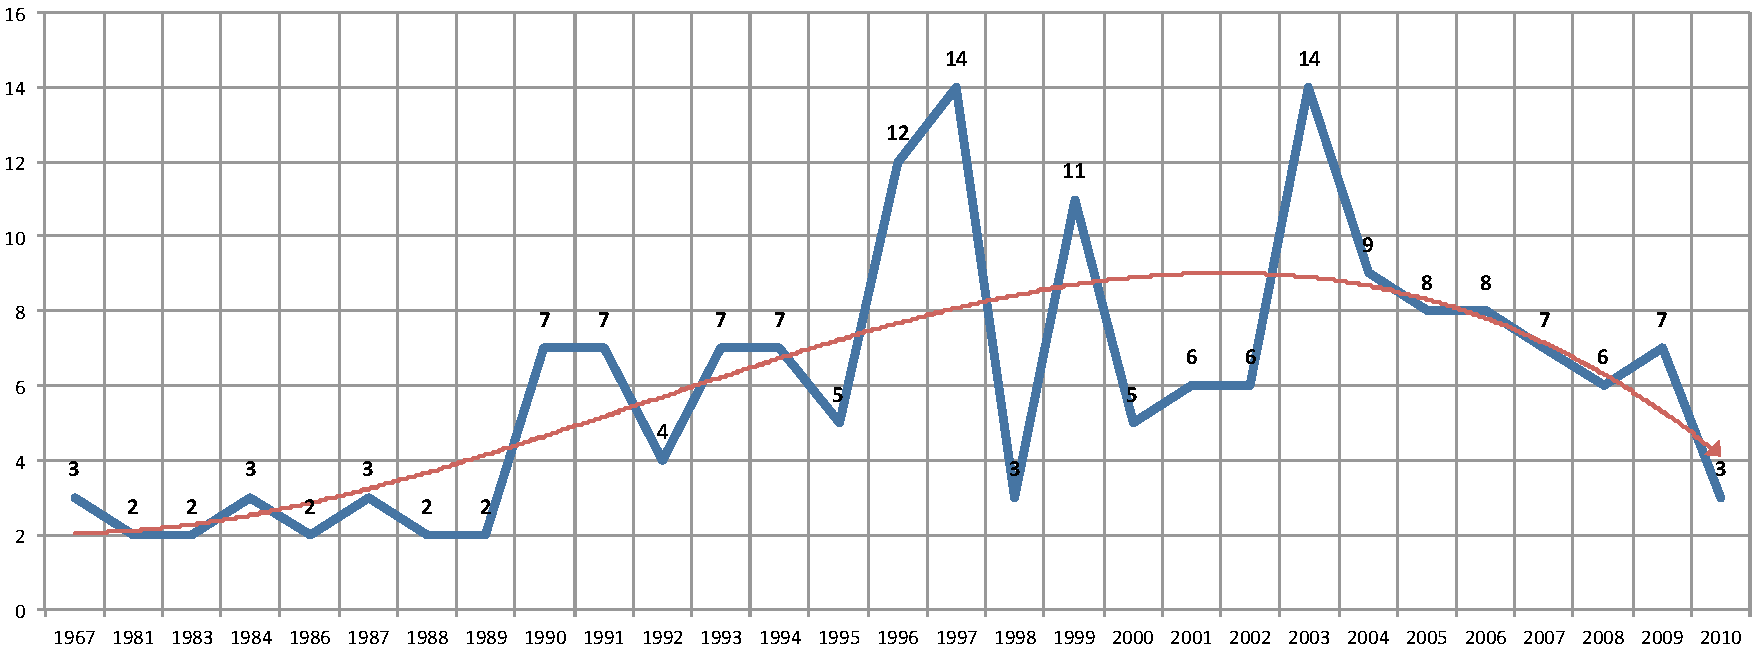
\includegraphics[scale=0.2]{A-figuras/abntex2-modelo-img-grafico.pdf} % utilize este comando para definir a escala da figura com relação ao original. Por exemplo, scale=1.0 significa tamanho original; scale=0.5 significa tamanho igual à metade do original; scale=0.73 significa tamanho igual a 73% do original
    \legend{Fonte: \citeonline[p. 24]{araujo2012}.} % utilize este comando para definir a fonte da figura, mesmo que seja de elaboração própria, indicando o ano de produção
  \end{minipage}
\end{figure}

Observe que, segundo a \citeonline[seção 5.8]{NBR14724:2024}, cada tipo de ilustração deve sempre ter numeração contínua e única em todo o documento:

\begin{citacao}
Qualquer tipo de ilustração deve ser precedido por sua palavra designativa (desenho, esquema, fluxograma, fotografia, gráfico, mapa, organograma, planta, quadro, retrato, figura, imagem, entre outros), seguida de seu número de ordem de ocorrência no texto, em algarismos arábicos, de travessão e do respectivo título.

Imediatamente após a ilustração, deve ser indicada a fonte consultada, conforme a ABNT NBR 10520, legenda, notas e, se houver, outras informações necessárias à sua compreensão. A ilustração produzida pelo autor, para o trabalho apresentado, deve conter na fonte esta informação: elaborado pelo próprio autor ou elaboração própria ou o próprio autor, entre outros.

A ilustração deve ser citada no texto e inserida o mais próximo possível do trecho a que se refere.

Tipo, número de ordem, título, fonte, legenda e notas devem acompanhar as margens da ilustração.
\end{citacao}

% ---
\section{Gráficos}
% ---
\index{gráficos}

O ambiente para a criação de gráficos é idêntico ao utilizado para a criação de figuras, conforme mostrado no \autoref{gra-excel}. Desse modo, vale para os gráficos tudo o que foi dito com relação às figuras.

\begin{grafico}[htb]
    \captionsetup{width=0.92\textwidth} % após a definição da escala XX da figura feita pelo comando \includegraphics[scale=XX] abaixo, ajuste o parâmetro width para posicionar corretamente o título e a fonte da figura alinhados com as margens da figura
    \caption{Gráfico produzido em Excel e salvo como PDF} % utilize este comando para definir o título da figura
    \label{gra-excel} % utilize este comando para definir o "apelido" da figura, que será utilizado para a citação da figura
    \vspace{-0.5cm}
    	\begin{center}
    	    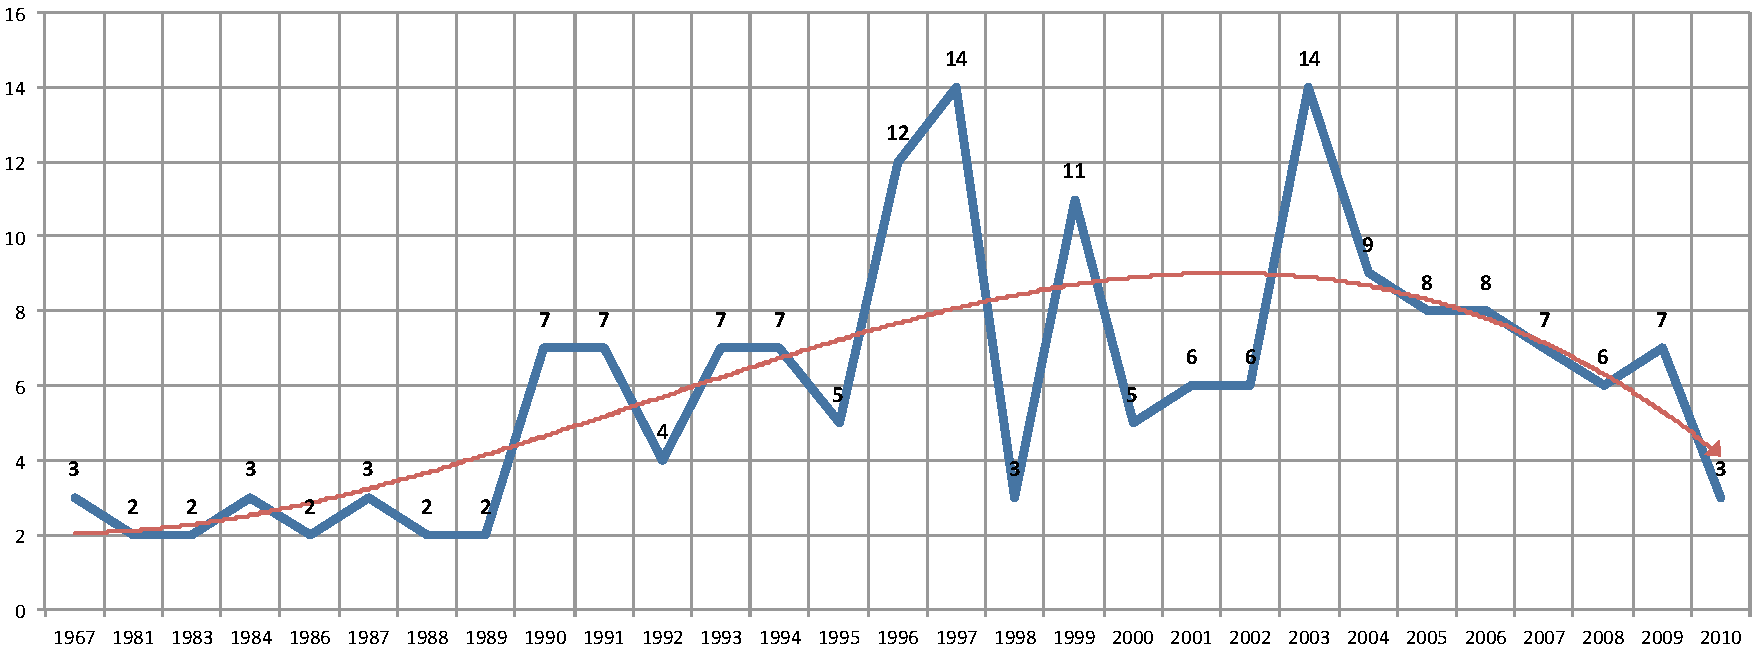
\includegraphics[scale=0.5]{A-figuras/abntex2-modelo-img-grafico.pdf} % utilize este comando para definir a escala da figura com relação ao original. Por exemplo, scale=1.0 significa tamanho original; scale=0.5 significa tamanho igual à metade do original; scale=0.73 significa tamanho igual a 73% do original
    	\end{center}
	\vspace{-0.5cm}
	\legend{Fonte: \citeonline[p. 24]{araujo2012}.} % utilize este comando para definir a fonte da figura, mesmo que seja de elaboração própria, indicando o ano de produção
\end{grafico}

% ---
\section{Quadros e tabelas}
% ---

Conforme \citeonline[seção 3.1]{ibge1993}, a tabela é uma forma ``não discursiva de apresentar informações, das quais o dado numérico se destaca como informação central'', definição corroborada por \citeonline[seção 3.32]{NBR14724:2024}.

Por outro lado, segundo a \citeonline[seção 3.21]{NBR14724:2024}, ilustração é a ``designação genérica de imagem, que ilustra ou elucida um texto''. Ademais, quadro é um tipo de ilustração \cite[seção 5.8]{NBR14724:2024}.

Isso significa que, perante essas normas, quadros e tabelas pertencem a tipos diferentes de elementos gráficos distintos do texto normal. Sendo assim, eles devem ter tratamento diferenciado, exigindo apresentações visuais diferentes.

Entende-se, então, complementarmente à definição anterior de tabela, que um quadro é uma forma não discursiva de apresentar informações, das quais o dado numérico não se destaca como informação central, mesmo que presente.

Além disso, para diferenciação visual, tabelas não possuem bordas verticais laterais; quadros possuem, sendo totalmente fechados por bordas, conforme os diversos exemplos apresentados a seguir.

% ---
\subsection{Quadros}
% ---

\index{quadros}O \autoref{qua-quadro1} exemplifica um quadro construído no ambiente \LaTeX.

\begin{quadro}[htb]
\IBGEtab{%
  \caption{Níveis de investigação} % utilize este comando para definir o título do quadro
  \label{qua-quadro1} % utilize este comando para definir o "apelido" do quadro, que será utilizado para a citação do quadro
}{%
\begin{tabular}{|m{2.6cm}|m{6.0cm}|m{2.25cm}|m{3.40cm}|}
    \hline
    \rowcolor{lightgray}
    \centering\textbf{Nível de Investigação} & \centering\textbf{Insumos}  & \centering\textbf{Sistemas de Investigação}  & \begin{center}\textbf{Produtos}\end{center} \\
    \hline
    Meta-nível & Filosofia\index{filosofia} da Ciência  & Epistemologia &
    Paradigma  \\
    \hline
    Nível do objeto & Paradigmas do metanível e evidências do nível inferior &
    Ciência  & Teorias e modelos \\
    \hline
    Nível inferior & Modelos e métodos do nível do objeto e problemas do nível inferior & Prática & Solução de problemas  \\
   \hline
\end{tabular}
}{
\legend{Fonte: \citeonline{van86}.} % utilize este comando para definir a fonte do quadro, mesmo que seja de elaboração própria, indicando o ano de produção
}
\end{quadro}

Por sua vez, o \autoref{qua-quadroTCC1} mostra como criar um quadro a partir de uma imagem. Neste caso, foi feita uma planilha em Excel, que foi copiada como imagem em formato PNG. Deve ser observado que a qualidade gráfica desta solução não é adequada.

\begin{quadro}[htb]
    \captionsetup{width=1.00\textwidth} % após a definição da escala XX do quadro feita pelo comando \includegraphics[scale=XX] abaixo, ajuste o parâmetro width para posicionar corretamente o título e a fonte do quadro alinhados com as margens do quadro
    \caption{Conceitos utilizados em referências associadas a trabalhos publicados em anais de eventos (Excel para Word para PNG)} % utilize este comando para definir o título do quadro
    \label{qua-quadroTCC1} % utilize este comando para definir o "apelido" do quadro, que será utilizado para a citação do quadro
    \vspace{-0.5cm}
    	\begin{center}
    	    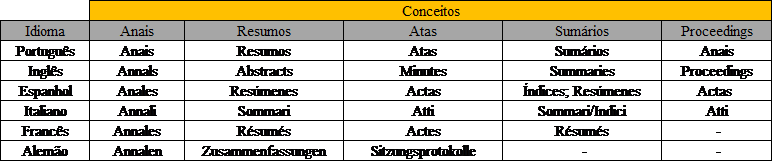
\includegraphics[scale=0.78]{A-figuras/quadroTCC.png} % utilize este comando para definir a escala do quadro com relação ao original. Por exemplo, scale=1.0 significa tamanho original; scale=0.5 significa tamanho igual à metade do original; scale=0.73 significa tamanho igual a 73% do original
    	\end{center}
	\vspace{-0.5cm}
	\fonte{elaboração própria (2023).} % utilize este comando para definir a fonte do quadro, mesmo que seja de elaboração própria
\end{quadro}

O \autoref{qua-quadroTCC2} encontra-se em \LaTeX, porém não foi criado neste ambiente. Ele foi gerado com o uso da página \url{https://www.tablesgenerator.com} e, depois, copiado e editado neste ambiente. Este é um recurso muito útil para a elaboração de quadros e tabelas mais complexos.
\index{url}

\begin{quadro}[!ht]
    \captionsetup{width=1.00\textwidth} % ajuste o parâmetro width para posicionar corretamente o título e a fonte do quadro alinhados com as margens do quadro
    \caption{Conceitos utilizados em referências associadas a trabalhos publicados em anais de eventos (\url{https://www.tablesgenerator.com})} % utilize este comando para definir o título do quadro
    \label{qua-quadroTCC2} % utilize este comando para definir o "apelido" do quadro, que será utilizado para a citação do quadro
\centering
\resizebox{\textwidth}{!}{%
\begin{tabular}{c|ccccc|}
\cline{2-6} &
\multicolumn{5}{c|}{\cellcolor[HTML]{FFC702}Conceitos} \\ \hline
\rowcolor[HTML]{9B9B9B} 
  \multicolumn{1}{|c|}{\cellcolor[HTML]{9B9B9B}Idioma} &
  \multicolumn{1}{c|}{\cellcolor[HTML]{9B9B9B}Anais} &
  \multicolumn{1}{c|}{\cellcolor[HTML]{9B9B9B}Resumos} &
  \multicolumn{1}{c|}{\cellcolor[HTML]{9B9B9B}Atas} &
  \multicolumn{1}{c|}{\cellcolor[HTML]{9B9B9B}Sumários} &
  Proceedings \\ \hline
\multicolumn{1}{|c|}{Português} &
  \multicolumn{1}{c|}{Anais} &
  \multicolumn{1}{c|}{Resumos} &
  \multicolumn{1}{c|}{Atas} &
  \multicolumn{1}{c|}{Sumários} &
  Anais \\ \hline
\multicolumn{1}{|c|}{Inglês} &
  \multicolumn{1}{c|}{Annals} &
  \multicolumn{1}{c|}{Abstracts} &
  \multicolumn{1}{c|}{Minutes} &
  \multicolumn{1}{c|}{Summaries} &
  Proceedings \\ \hline
\multicolumn{1}{|c|}{Espanhol} &
  \multicolumn{1}{c|}{Anales} &
  \multicolumn{1}{c|}{Resúmenes} &
  \multicolumn{1}{c|}{Actas} &
  \multicolumn{1}{c|}{Índices; Resúmenes} &
  Actas \\ \hline
\multicolumn{1}{|c|}{Italiano} &
  \multicolumn{1}{c|}{Annali} &
  \multicolumn{1}{c|}{Sommari} &
  \multicolumn{1}{c|}{Atti} &
  \multicolumn{1}{c|}{Sommari/ Indici} &
  Atti \\ \hline
\multicolumn{1}{|c|}{Francês} &
  \multicolumn{1}{c|}{Annales} &
  \multicolumn{1}{c|}{Résumés} &
  \multicolumn{1}{c|}{Actes} &
  \multicolumn{1}{c|}{Résumés} &
  - \\ \hline
\multicolumn{1}{|c|}{Alemão} &
  \multicolumn{1}{c|}{Annalen} &
  \multicolumn{1}{c|}{Zusammenfassungen} &
  \multicolumn{1}{c|}{Sitzungsprotokolle} &
  \multicolumn{1}{c|}{-} &
  - \\ \hline
\end{tabular}%
}
    \fonte{elaboração própria (2023).} % utilize este comando para definir a fonte do quadro, mesmo que seja de elaboração própria
\end{quadro}

O \autoref{qua-quadroTCC-ppt} também mostra como criar um quadro a partir de uma imagem. Neste caso, foi feita uma planilha em Excel, que foi copiada para o PowerPoint, de onde foi copiada como imagem no formato PNG. A qualidade gráfica desta solução é bem melhor que a mostrada no \autoref{qua-quadroTCC1}.

Conforme se pode ver, a largura do quadro não é a mais adequada ao formato da página: A4 em orientação retrato. Em função disso, foi criado o \autoref{qua-quadroTCC-ppt2}, que altera a orientação da respectiva página para paisagem. Essa nova configuração melhora a qualidade visual do quadro.

\begin{quadro}[htb]
    \captionsetup{width=1.00\textwidth} % após a definição da escala XX do quadro feita pelo comando \includegraphics[scale=XX] abaixo, ajuste o parâmetro width para posicionar corretamente o título e a fonte do quadro alinhados com as margens do quadro
    \caption{Cronograma do processo seletivo de 2023 para alunos do MPPL (PSAR 2023)} % utilize este comando para definir o título do quadro
    \label{qua-quadroTCC-ppt} % utilize este comando para definir o "apelido" do quadro, que será utilizado para a citação do quadro
    \vspace{-0.5cm}
    	\begin{center}
    	    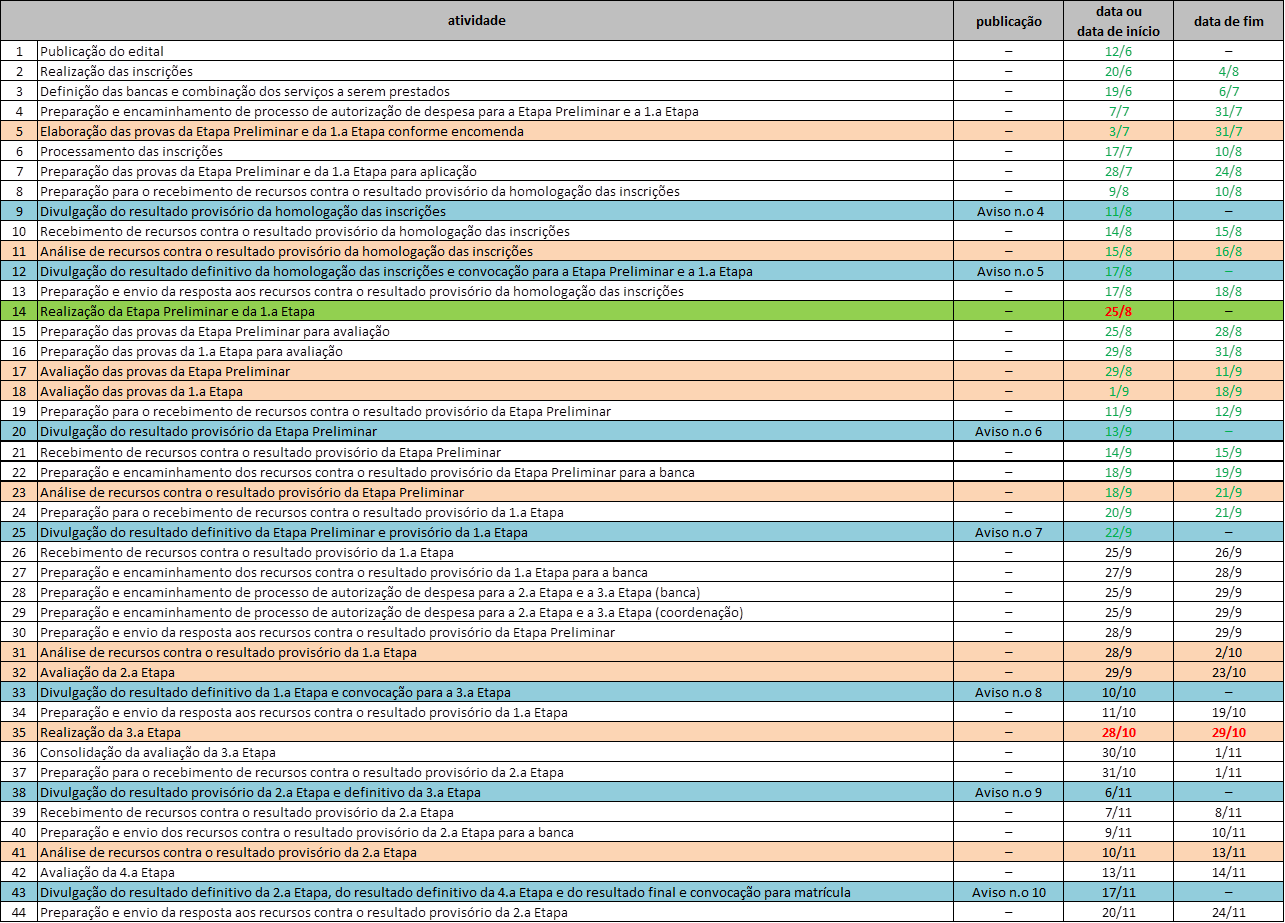
\includegraphics[scale=0.70]{A-figuras/psar 2023-ppt.png} % utilize este comando para definir a escala do quadro com relação ao original. Por exemplo, scale=1.0 significa tamanho original; scale=0.5 significa tamanho igual à metade do original; scale=0.73 significa tamanho igual a 73% do original
    	\end{center}
	\vspace{-0.5cm}
	\fonte{elaboração própria (2024).} % utilize este comando para definir a fonte do quadro, mesmo que seja de elaboração própria
\end{quadro}

O \autoref{qua-crono} mostra a melhor solução para o caso: código em \LaTeX, elaborado com o uso da página \url{https://www.tablesgenerator.com} e, depois, copiado e editado neste ambiente, a mesma estratégia utilizada para o \autoref{qua-quadroTCC2}.

\begin{landscape}
\begin{quadro}[htb]
    \captionsetup{width=0.81\linewidth} % após a definição da escala XX do quadro feita pelo comando \includegraphics[scale=XX] abaixo, ajuste o parâmetro width para posicionar corretamente o título e a fonte do quadro alinhados com as margens do quadro
    \caption{Cronograma do processo seletivo de 2023 para alunos do MPPL (PSAR 2023)} % utilize este comando para definir o título do quadro
    \label{qua-quadroTCC-ppt2} % utilize este comando para definir o "apelido" do quadro, que será utilizado para a citação do quadro
    \vspace{-0.5cm}
    	\begin{center}
    	    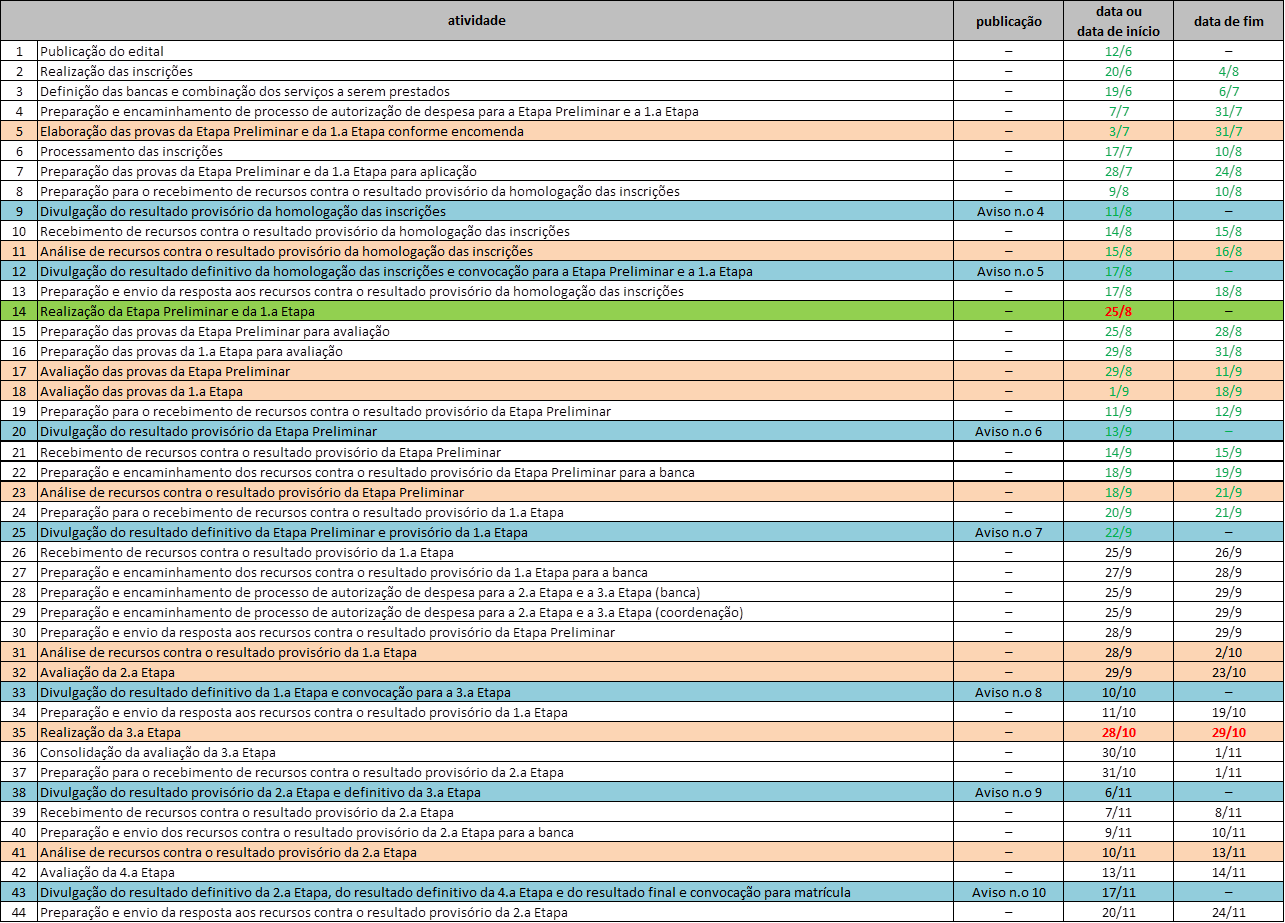
\includegraphics[scale=0.88]{A-figuras/psar 2023-ppt.png} % utilize este comando para definir a escala do quadro com relação ao original. Por exemplo, scale=1.0 significa tamanho original; scale=0.5 significa tamanho igual à metade do original; scale=0.73 significa tamanho igual a 73% do original
    	\end{center}
	\vspace{-0.5cm}
	\fonte{elaboração própria (2024).} % utilize este comando para definir a fonte do quadro, mesmo que seja de elaboração própria
\end{quadro}
\end{landscape}


\begin{landscape}
\begin{quadro}[htb]
\centering
\captionsetup{width=0.98\linewidth} % ajuste o parâmetro width para posicionar corretamente o título e a fonte do quadro alinhados com as margens do quadro
\caption{Cronograma do processo seletivo de 2023 para alunos do MPPL (PSAR 2023)}
\label{qua-crono}
\begin{adjustbox}{max width=0.98\linewidth} 

\begin{tabular}{|c|l|c|c|c|c|c|}
\hline
\rowcolor[HTML]{BFBFBF} 
\multicolumn{2}{|c|}{\cellcolor[HTML]{BFBFBF}\textbf{atividade}}                                                                                  & \textbf{publicação} & \textbf{\begin{tabular}[c]{@{}c@{}}data ou \\      data de início\end{tabular}} & \textbf{data de fim}                  & \textbf{\begin{tabular}[c]{@{}c@{}}data ou \\      data de início\end{tabular}} & \textbf{data de fim} \\ \hline
1  & Publicação do edital                                                                                                                       & –                   & 12/6                                                                            & –                                     & 6/6                                                                             & –                    \\
2  & Realização das   inscrições                                                                                                                & –                   & 20/6                                                                            & 4/8                                   & 7/6                                                                             & 1/7                  \\
3  & Definição das bancas   e combinação dos serviços a serem prestados                                                                         & –                   & 19/6                                                                            & 6/7                                   & 27/6                                                                            & 5/7                  \\
4  & Preparação e   encaminhamento de processo de autorização de despesa para a Etapa Preliminar   e a 1.a Etapa                                & –                   & 7/7                                                                             & 31/7                                  & 6/7                                                                             & 4/8                  \\
\rowcolor[HTML]{FCD5B4} 
5  & Elaboração das provas   da Etapa Preliminar e da 1.a Etapa conforme encomenda                                                              & –                   & 3/7                                                                             & 31/7                                  & 6/7                                                                             & 25/7                 \\
6  & Processamento das   inscrições                                                                                                             & –                   & 17/7                                                                            & 10/8                                  & 4/7                                                                             & 28/7                 \\
7  & Preparação das provas   da Etapa Preliminar e da 1.a Etapa para aplicação                                                                  & –                   & 28/7                                                                            & 24/8                                  & 26/7                                                                            & 11/8                 \\
8  & Preparação para o   recebimento de recursos contra o resultado provisório da homologação das   inscrições                                  & –                   & 9/8                                                                             & 10/8                                  & 26/7                                                                            & 29/7                 \\
\rowcolor[HTML]{92CDDC} 
9  & Divulgação do   resultado provisório da homologação das inscrições                                                                         & Aviso n.o 4         & 11/8                                                                            & –                                     & 29/7                                                                            & –                    \\
10 & Recebimento de   recursos contra o resultado provisório da homologação das inscrições                                                      & –                   & 14/8                                                                            & 15/8                                  & 1/8                                                                             & 2/8                  \\
\rowcolor[HTML]{FCD5B4} 
11 & Análise de recursos   contra o resultado provisório da homologação das inscrições                                                          & –                   & 15/8                                                                            & 16/8                                  & 2/8                                                                             & 3/8                  \\
\rowcolor[HTML]{92CDDC} 
12 & Divulgação do   resultado definitivo da homologação das inscrições e convocação para a Etapa   Preliminar e a 1.a Etapa                    & Aviso n.o 5         & 17/8                                                                            & –                                     & 4/8                                                                             & –                    \\
13 & Preparação e envio da   resposta aos recursos contra o resultado provisório da homologação das   inscrições                                & –                   & 17/8                                                                            & 18/8                                  & 4/8                                                                             & 5/8                  \\
\rowcolor[HTML]{92D050} 
14 & Realização da Etapa   Preliminar e da 1.a Etapa                                                                                            & –                   & {\color[HTML]{FF0000} \textbf{25/8}}                                            & –                                     & 12/8                                                                            & –                    \\
15 & Preparação das provas   da Etapa Preliminar para avaliação                                                                                 & –                   & 25/8                                                                            & 28/8                                  & 12/8                                                                            & 15/8                 \\
16 & Preparação das provas   da 1.a Etapa para avaliação                                                                                        & –                   & 29/8                                                                            & 31/8                                  & 16/8                                                                            & 19/8                 \\
\rowcolor[HTML]{FCD5B4} 
17 & Avaliação das provas   da Etapa Preliminar                                                                                                 & –                   & 29/8                                                                            & 11/9                                  & 16/8                                                                            & 29/8                 \\
\rowcolor[HTML]{FCD5B4} 
18 & Avaliação das provas   da 1.a Etapa                                                                                                        & –                   & 1/9                                                                             & 18/9                                  & 17/8                                                                            & 5/9                  \\
19 & Preparação para o   recebimento de recursos contra o resultado provisório da Etapa Preliminar                                              & –                   & 11/9                                                                            & 12/9                                  & 29/8                                                                            & 30/8                 \\
\rowcolor[HTML]{92CDDC} 
20 & Divulgação do   resultado provisório da Etapa Preliminar                                                                                   & Aviso n.o 6         & 13/9                                                                            & –                                     & 31/8                                                                            & –                    \\
21 & Recebimento de   recursos contra o resultado provisório da Etapa Preliminar                                                                & –                   & 14/9                                                                            & 15/9                                  & 1/9                                                                             & 2/9                  \\
22 & Preparação e   encaminhamento dos recursos contra o resultado provisório da Etapa Preliminar   para a banca                                & –                   & 18/9                                                                            & 19/9                                  & 5/9                                                                             & 5/9                  \\
\rowcolor[HTML]{FCD5B4} 
23 & Análise de recursos   contra o resultado provisório da Etapa Preliminar                                                                    & –                   & 18/9                                                                            & 21/9                                  & 5/9                                                                             & 8/9                  \\
24 & Preparação para o   recebimento de recursos contra o resultado provisório da 1.a Etapa                                                     & –                   & 20/9                                                                            & 21/9                                  & 6/9                                                                             & 8/9                  \\
\rowcolor[HTML]{92CDDC} 
25 & Divulgação do   resultado definitivo da Etapa Preliminar e provisório da 1.a Etapa                                                         & Aviso n.o 7         & 22/9                                                                            & –                                     & 9/9                                                                             & –                    \\
26 & Recebimento de   recursos contra o resultado provisório da 1.a Etapa                                                                       & –                   & 25/9                                                                            & 26/9                                  & 12/9                                                                            & 13/9                 \\
27 & Preparação e   encaminhamento dos recursos contra o resultado provisório da 1.a Etapa para a   banca                                       & –                   & 27/9                                                                            & 28/9                                  & 14/9                                                                            & 15/9                 \\
28 & Preparação e   encaminhamento de processo de autorização de despesa para a 2.a Etapa e a 3.a   Etapa (banca)                               & –                   & 25/9                                                                            & 29/9                                  & 28/9                                                                            & 6/10                 \\
29 & Preparação e   encaminhamento de processo de autorização de despesa para a 2.a Etapa e a 3.a   Etapa (coordenação)                         & –                   & 25/9                                                                            & 29/9                                  & 10/10                                                                           & 20/10                \\
30 & Preparação e envio da   resposta aos recursos contra o resultado provisório da Etapa Preliminar                                            & –                   & 28/9                                                                            & 29/9                                  & 12/9                                                                            & 13/9                 \\
\rowcolor[HTML]{FCD5B4} 
31 & Análise de recursos   contra o resultado provisório da 1.a Etapa                                                                           & –                   & 28/9                                                                            & 2/10                                  & 15/9                                                                            & 18/9                 \\
\rowcolor[HTML]{FCD5B4} 
32 & Avaliação da 2.a   Etapa                                                                                                                   & –                   & 29/9                                                                            & 23/10                                 & 16/9                                                                            & 15/10                \\
\rowcolor[HTML]{92CDDC} 
33 & Divulgação do   resultado definitivo da 1.a Etapa e convocação para a 3.a Etapa                                                            & Aviso n.o 8         & 10/10                                                                           & –                                     & 27/9                                                                            & –                    \\
34 & Preparação e envio da   resposta aos recursos contra o resultado provisório da 1.a Etapa                                                   & –                   & 11/10                                                                           & 19/10                                 & 28/9                                                                            & 7/10                 \\
\rowcolor[HTML]{FCD5B4} 
35 & Realização da 3.a   Etapa                                                                                                                  & –                   & {\color[HTML]{FF0000} \textbf{28/10}}                                           & {\color[HTML]{FF0000} \textbf{29/10}} & 22/10                                                                           & 23/10                \\
36 & Consolidação da   avaliação da 3.a Etapa                                                                                                   & –                   & 30/10                                                                           & 1/11                                  & 24/10                                                                           & 3/11                 \\
37 & Preparação para o   recebimento de recursos contra o resultado provisório da 2.a Etapa                                                     & –                   & 31/10                                                                           & 1/11                                  & 1/11                                                                            & 3/11                 \\
\rowcolor[HTML]{92CDDC} 
38 & Divulgação do   resultado provisório da 2.a Etapa e definitivo da 3.a Etapa                                                                & Aviso n.o 9         & 6/11                                                                            & –                                     & 4/11                                                                            & –                    \\
39 & Recebimento de   recursos contra o resultado provisório da 2.a Etapa                                                                       & –                   & 7/11                                                                            & 8/11                                  & 7/11                                                                            & 8/11                 \\
40 & Preparação e envio   dos recursos contra o resultado provisório da 2.a Etapa para a banca                                                  & –                   & 9/11                                                                            & 10/11                                 & 9/11                                                                            & 9/11                 \\
\rowcolor[HTML]{FCD5B4} 
41 & Análise de recursos   contra o resultado provisório da 2.a Etapa                                                                           & –                   & 10/11                                                                           & 13/11                                 & 9/11                                                                            & 10/11                \\
42 & Avaliação da 4.a   Etapa                                                                                                                   & –                   & 13/11                                                                           & 14/11                                 & 9/11                                                                            & 10/11                \\
\rowcolor[HTML]{92CDDC} 
43 & Divulgação do   resultado definitivo da 2.a Etapa, do resultado definitivo da 4.a Etapa e do   resultado final e convocação para matrícula & Aviso n.o 10        & 17/11                                                                           & –                                     & 11/11                                                                           & –                    \\
44 & Preparação e envio da   resposta aos recursos contra o resultado provisório da 2.a Etapa                                                   & –                   & 20/11                                                                           & 24/11                                 & 14/11                                                                           & 18/11 \\      \hline        
\end{tabular}

\end{adjustbox}
\fonte{elaboração própria (2024).} % utilize este comando para definir a fonte do quadro, mesmo que seja de elaboração própria
\end{quadro}
\end{landscape}

O \autoref{qua-crono2} foi construído da mesma forma que o \autoref{qua-crono}, mas para impressão no formato retrato. Como se pode ver, a diagramação fica perfeita, mas com redução da fonte utilizada, para que o quadro não extrapole a largura do texto na página.

\begin{quadro}[htb]
\centering
\captionsetup{width=1.0\linewidth} % ajuste o parâmetro width para posicionar corretamente o título e a fonte do quadro alinhados com as margens do quadro
\caption{Cronograma do processo seletivo de 2023 para alunos do MPPL (PSAR 2023)}
\label{qua-crono2}
\begin{adjustbox}{max width=1.0\linewidth}

\begin{tabular}{|c|l|c|c|c|c|c|}
\hline
\rowcolor[HTML]{BFBFBF} 
\multicolumn{2}{|c|}{\cellcolor[HTML]{BFBFBF}\textbf{atividade}}                                                                                  & \textbf{publicação} & \textbf{\begin{tabular}[c]{@{}c@{}}data ou \\      data de início\end{tabular}} & \textbf{data de fim}                  & \textbf{\begin{tabular}[c]{@{}c@{}}data ou \\      data de início\end{tabular}} & \textbf{data de fim} \\ \hline
1  & Publicação do edital                                                                                                                       & –                   & 12/6                                                                            & –                                     & 6/6                                                                             & –                    \\
2  & Realização das   inscrições                                                                                                                & –                   & 20/6                                                                            & 4/8                                   & 7/6                                                                             & 1/7                  \\
3  & Definição das bancas   e combinação dos serviços a serem prestados                                                                         & –                   & 19/6                                                                            & 6/7                                   & 27/6                                                                            & 5/7                  \\
4  & Preparação e   encaminhamento de processo de autorização de despesa para a Etapa Preliminar   e a 1.a Etapa                                & –                   & 7/7                                                                             & 31/7                                  & 6/7                                                                             & 4/8                  \\
\rowcolor[HTML]{FCD5B4} 
5  & Elaboração das provas   da Etapa Preliminar e da 1.a Etapa conforme encomenda                                                              & –                   & 3/7                                                                             & 31/7                                  & 6/7                                                                             & 25/7                 \\
6  & Processamento das   inscrições                                                                                                             & –                   & 17/7                                                                            & 10/8                                  & 4/7                                                                             & 28/7                 \\
7  & Preparação das provas   da Etapa Preliminar e da 1.a Etapa para aplicação                                                                  & –                   & 28/7                                                                            & 24/8                                  & 26/7                                                                            & 11/8                 \\
8  & Preparação para o   recebimento de recursos contra o resultado provisório da homologação das   inscrições                                  & –                   & 9/8                                                                             & 10/8                                  & 26/7                                                                            & 29/7                 \\
\rowcolor[HTML]{92CDDC} 
9  & Divulgação do   resultado provisório da homologação das inscrições                                                                         & Aviso n.o 4         & 11/8                                                                            & –                                     & 29/7                                                                            & –                    \\
10 & Recebimento de   recursos contra o resultado provisório da homologação das inscrições                                                      & –                   & 14/8                                                                            & 15/8                                  & 1/8                                                                             & 2/8                  \\
\rowcolor[HTML]{FCD5B4} 
11 & Análise de recursos   contra o resultado provisório da homologação das inscrições                                                          & –                   & 15/8                                                                            & 16/8                                  & 2/8                                                                             & 3/8                  \\
\rowcolor[HTML]{92CDDC} 
12 & Divulgação do   resultado definitivo da homologação das inscrições e convocação para a Etapa   Preliminar e a 1.a Etapa                    & Aviso n.o 5         & 17/8                                                                            & –                                     & 4/8                                                                             & –                    \\
13 & Preparação e envio da   resposta aos recursos contra o resultado provisório da homologação das   inscrições                                & –                   & 17/8                                                                            & 18/8                                  & 4/8                                                                             & 5/8                  \\
\rowcolor[HTML]{92D050} 
14 & Realização da Etapa   Preliminar e da 1.a Etapa                                                                                            & –                   & {\color[HTML]{FF0000} \textbf{25/8}}                                            & –                                     & 12/8                                                                            & –                    \\
15 & Preparação das provas   da Etapa Preliminar para avaliação                                                                                 & –                   & 25/8                                                                            & 28/8                                  & 12/8                                                                            & 15/8                 \\
16 & Preparação das provas   da 1.a Etapa para avaliação                                                                                        & –                   & 29/8                                                                            & 31/8                                  & 16/8                                                                            & 19/8                 \\
\rowcolor[HTML]{FCD5B4} 
17 & Avaliação das provas   da Etapa Preliminar                                                                                                 & –                   & 29/8                                                                            & 11/9                                  & 16/8                                                                            & 29/8                 \\
\rowcolor[HTML]{FCD5B4} 
18 & Avaliação das provas   da 1.a Etapa                                                                                                        & –                   & 1/9                                                                             & 18/9                                  & 17/8                                                                            & 5/9                  \\
19 & Preparação para o   recebimento de recursos contra o resultado provisório da Etapa Preliminar                                              & –                   & 11/9                                                                            & 12/9                                  & 29/8                                                                            & 30/8                 \\
\rowcolor[HTML]{92CDDC} 
20 & Divulgação do   resultado provisório da Etapa Preliminar                                                                                   & Aviso n.o 6         & 13/9                                                                            & –                                     & 31/8                                                                            & –                    \\
21 & Recebimento de   recursos contra o resultado provisório da Etapa Preliminar                                                                & –                   & 14/9                                                                            & 15/9                                  & 1/9                                                                             & 2/9                  \\
22 & Preparação e   encaminhamento dos recursos contra o resultado provisório da Etapa Preliminar   para a banca                                & –                   & 18/9                                                                            & 19/9                                  & 5/9                                                                             & 5/9                  \\
\rowcolor[HTML]{FCD5B4} 
23 & Análise de recursos   contra o resultado provisório da Etapa Preliminar                                                                    & –                   & 18/9                                                                            & 21/9                                  & 5/9                                                                             & 8/9                  \\
24 & Preparação para o   recebimento de recursos contra o resultado provisório da 1.a Etapa                                                     & –                   & 20/9                                                                            & 21/9                                  & 6/9                                                                             & 8/9                  \\
\rowcolor[HTML]{92CDDC} 
25 & Divulgação do   resultado definitivo da Etapa Preliminar e provisório da 1.a Etapa                                                         & Aviso n.o 7         & 22/9                                                                            & –                                     & 9/9                                                                             & –                    \\
26 & Recebimento de   recursos contra o resultado provisório da 1.a Etapa                                                                       & –                   & 25/9                                                                            & 26/9                                  & 12/9                                                                            & 13/9                 \\
27 & Preparação e   encaminhamento dos recursos contra o resultado provisório da 1.a Etapa para a   banca                                       & –                   & 27/9                                                                            & 28/9                                  & 14/9                                                                            & 15/9                 \\
28 & Preparação e   encaminhamento de processo de autorização de despesa para a 2.a Etapa e a 3.a   Etapa (banca)                               & –                   & 25/9                                                                            & 29/9                                  & 28/9                                                                            & 6/10                 \\
29 & Preparação e   encaminhamento de processo de autorização de despesa para a 2.a Etapa e a 3.a   Etapa (coordenação)                         & –                   & 25/9                                                                            & 29/9                                  & 10/10                                                                           & 20/10                \\
30 & Preparação e envio da   resposta aos recursos contra o resultado provisório da Etapa Preliminar                                            & –                   & 28/9                                                                            & 29/9                                  & 12/9                                                                            & 13/9                 \\
\rowcolor[HTML]{FCD5B4} 
31 & Análise de recursos   contra o resultado provisório da 1.a Etapa                                                                           & –                   & 28/9                                                                            & 2/10                                  & 15/9                                                                            & 18/9                 \\
\rowcolor[HTML]{FCD5B4} 
32 & Avaliação da 2.a   Etapa                                                                                                                   & –                   & 29/9                                                                            & 23/10                                 & 16/9                                                                            & 15/10                \\
\rowcolor[HTML]{92CDDC} 
33 & Divulgação do   resultado definitivo da 1.a Etapa e convocação para a 3.a Etapa                                                            & Aviso n.o 8         & 10/10                                                                           & –                                     & 27/9                                                                            & –                    \\
34 & Preparação e envio da   resposta aos recursos contra o resultado provisório da 1.a Etapa                                                   & –                   & 11/10                                                                           & 19/10                                 & 28/9                                                                            & 7/10                 \\
\rowcolor[HTML]{FCD5B4} 
35 & Realização da 3.a   Etapa                                                                                                                  & –                   & {\color[HTML]{FF0000} \textbf{28/10}}                                           & {\color[HTML]{FF0000} \textbf{29/10}} & 22/10                                                                           & 23/10                \\
36 & Consolidação da   avaliação da 3.a Etapa                                                                                                   & –                   & 30/10                                                                           & 1/11                                  & 24/10                                                                           & 3/11                 \\
37 & Preparação para o   recebimento de recursos contra o resultado provisório da 2.a Etapa                                                     & –                   & 31/10                                                                           & 1/11                                  & 1/11                                                                            & 3/11                 \\
\rowcolor[HTML]{92CDDC} 
38 & Divulgação do   resultado provisório da 2.a Etapa e definitivo da 3.a Etapa                                                                & Aviso n.o 9         & 6/11                                                                            & –                                     & 4/11                                                                            & –                    \\
39 & Recebimento de   recursos contra o resultado provisório da 2.a Etapa                                                                       & –                   & 7/11                                                                            & 8/11                                  & 7/11                                                                            & 8/11                 \\
40 & Preparação e envio   dos recursos contra o resultado provisório da 2.a Etapa para a banca                                                  & –                   & 9/11                                                                            & 10/11                                 & 9/11                                                                            & 9/11                 \\
\rowcolor[HTML]{FCD5B4} 
41 & Análise de recursos   contra o resultado provisório da 2.a Etapa                                                                           & –                   & 10/11                                                                           & 13/11                                 & 9/11                                                                            & 10/11                \\
42 & Avaliação da 4.a   Etapa                                                                                                                   & –                   & 13/11                                                                           & 14/11                                 & 9/11                                                                            & 10/11                \\
\rowcolor[HTML]{92CDDC} 
43 & Divulgação do   resultado definitivo da 2.a Etapa, do resultado definitivo da 4.a Etapa e do   resultado final e convocação para matrícula & Aviso n.o 10        & 17/11                                                                           & –                                     & 11/11                                                                           & –                    \\
44 & Preparação e envio da   resposta aos recursos contra o resultado provisório da 2.a Etapa                                                   & –                   & 20/11                                                                           & 24/11                                 & 14/11                                                                           & 18/11 \\      \hline        
\end{tabular}


\end{adjustbox}
\fonte{elaboração própria (2024).} % utilize este comando para definir a fonte do quadro, mesmo que seja de elaboração própria
\end{quadro}


O \autoref{qua-bib-ag-camara} exemplifica o uso de um quadro longo, que utiliza duas ou mais páginas do documento. Este exemplo é importante porque utiliza o ambiente \verb|longtable|, que é diferente do já utilizado \verb|table|. Ele necessita de informações especiais para configurar os cabeçalhos da primeira página e das demais páginas. No caso de necessidade de se utilizar um quadro longo, sugere-se editar este exemplo, adaptando-o ao caso concreto.

 \begin{quadro}[htbp]
  \centering
  \captionsetup{width=1.\textwidth} % comando necessário para posicionar corretamente o título e a fonte da figura: parâmetro width deve ser igual ao do comando \includegraphics a seguir
  \caption{Descrição de artigos, monografias, dissertações e teses sobre a Agência Câmara}
  \label{qua-bib-ag-camara}  
\end{quadro}
\vspace{-12mm}
           
\begingroup
\footnotesize
\setlength{\tabcolsep}{3pt} % Valor padrão é 6pt

\begin{longtable}{|m{0.28\textwidth}|m{0.14\textwidth}|m{0.15\textwidth}|m{0.13\textwidth}|m{0.16\textwidth}|>{\centering\arraybackslash}p{0.05\textwidth}|}
\multicolumn{6}{r}{(continua)}\\
\hline
\rowcolor[HTML]{BFBFBF} \centering \textbf{Título}\tablefootnote{Exemplo de nota de rodapé em cabeçalho de quadro longo.} & \centering \textbf{Categoria} & \centering \textbf{Publicação/ Instituição} & \centering \textbf{Área} & \centering \textbf{Autor(a)} & \multicolumn{1}{c|}{\textbf{Ano}}\\
\hline
\endfirsthead
\multicolumn{6}{l}{\small \vspace{-0.5mm}\hspace{-2.75mm} \textbf{\autoref{qua-bib-ag-camara}} \normalsize -- \small Descrição de artigos, monografias, dissertações e teses sobre a Agência Câmara}\\
\multicolumn{6}{r}{(continuação)}\\
\hline
\rowcolor[HTML]{BFBFBF} \centering \textbf{Título} & \centering \textbf{Categoria} & \centering \textbf{Publicação/ Instituição} & \centering \textbf{Área} & \centering \textbf{Autor(a)} & \multicolumn{1}{c|}{\textbf{Ano}}\\
\hline
\endhead

A mediação da assessoria de   imprensa parlamentar nas relações de poder entre o Legislativo e o Executivo\tablefootnote{Exemplo de nota de rodapé em corpo de quadro longo.} & Dissertação & UFSC & Sociologia & FRANZONI, Sabrina & 2005 \\ \hline
A informação legislativa da fonte   ao veículo: análise crítica sobre os processos de articulação entre a   Consultoria Legislativa e a Secretaria de Comunicação da Câmara dos Deputados & Monografia & Cefor (Câmara dos Deputados) & Ciência Política & QUEIROZ, Cid Medeiros Cavalcanti de & 2007 \\ \hline
A mídia legislativa como estratégia   de conexão eleitoral dos parlamentares brasileiros: o caso da Câmara dos   Deputados & Artigo & Encontro Anual da   Associação Nacional de Pós-Graduação & Ciência Política & BARROS, Antônio Teixeira de;   BERNARDES, Cristiane Brum & 2007 \\ \hline
A cobertura jornalística na Câmara   dos Deputados & Artigo & Revista E-Legis   (Cefor/Câmara dos Deputados) & Ciência Política & ROCHA, Candyce da Cruz & 2009 \\ \hline
Política, institucional ou pública?   Uma reflexão sobre a mídia legislativa da Câmara dos Deputados & Tese & UERJ & Ciência Política & BERNARDES, Cristiane Brum & 2010 \\ \hline
Pessoas com deficiência: a   trajetória de um tema na agenda pública & Dissertação & UnB & Ciência Política & MONTEIRO, Adriana Resende & 2010 \\ \hline
As Fontes de Informação nas Mídias   Legislativas: oficialismo e diversidade na produção noticiosa sobre a Câmara   dos Deputados & Artigo & Brazilian Journalism   Research (revista da SBPJOR) & Comunicação & BERNARDES, Cristiane Brum & 2011 \\ \hline
Fatos X Opiniões: a linguagem   jornalística nas mídias legislativas da Câmara dos Deputados brasileira & Artigo & Estudos em Comunicação   (Universidade da Beira Interior/POR) & Comunicação & BERNARDES, Cristiane Brum & 2011 \\ \hline
Critérios de noticiabilidade e   pauta da mídia legislativa da Câmara dos Deputados & Artigo & Intexto (UFRGS) & Comunicação & BERNARDES, Cristiane Brum & 2011 \\ \hline
Código florestal, reserva legal e   comunicação ambiental: análise das ofertas nas mídias legislativas federais & Dissertação & Universidade Vale do   Taquari & Ambiente e Desenvolvimento & LUZ, Josiane Paula Da & 2012 \\ \hline
Indexação e taxonomia em sites de   webjornalismo: um estudo para aprimorar a recuperação de informação no Portal   Câmara Notícias & Monografia & UFMG & Arquitetura e Organização   da Informação & OLIVEIRA, Marcos Adriano Rossi de & 2013 \\ \hline
Mudanças nas rotinas de produção do   jornalismo da Câmara dos Deputados: o processo de integração das mídias   legislativas & Artigo & Contemporânea: Revista de   Comunicação e Cultura (UFBA) & Comunicação & BERNARDES, C. B.; MACEDO, S.M. & 2014 \\ \hline
Estratégias da Câmara dos Deputados   para a inserção social de conteúdos políticos e culturais & Artigo & Revista Estudos   Legislativos (Assembleia Legislativa do Rio Grande do Sul) & Ciência Política & BARROS, Antonio Teixeira de;   MENEGUIN, Ana Marusia Pinheiro & 2015 \\ \hline
Public Communication in the   Brazilian Congress: The News Agency and TV Station of the Chamber of Deputies & Artigo & Latin American research review   (Cambridge University) & Comunicação & LEMOS, Cláudia R. F.; BERNARDES,   Cristiane B.; BARROS, Antonio & 2016 \\ \hline
A cobertura jornalística em mídias   legislativas: um estudo sobre a Agência Câmara & Artigo & RECP: Revista Eletrônica de   Ciência Política (UFPR) & Comunicação & NOGUEIRA, Leidyanne V.; MARQUES,   Francisco Paulo Jamil & 2016 \\ \hline
As manifestações de 2013 sob a   ótica da Câmara dos Deputados: a Agência Câmara de Notícias na abordagem de   uma temática nacional & Monografia & Cefor (Câmara dos Deputados) & Comunicação & PAIVA, Mariana Macedo Lahud & 2016 \\ \hline
Interesse público em mídias   legislativas: um estudo da produção noticiosa da Agência Câmara Notícias & Dissertação & UFC & Comunicação & NOGUEIRA, Leidyanne Viana & 2017 \\ \hline
Mídia legislativa e representação   de gênero na Câmara dos Deputados: uma análise das notícias da Agência Câmara & Dissertação & Cefor (Câmara dos Deputados) & Ciência Política & ABREU, Mariana Silva & 2017 \\ \hline
Jornalismo   e Interesse Público: uma análise da Agência Câmara Notícias a partir da   categorização de fatos & Artigo & Âncora: Revista   Latino-americana de jornalismo (UFPB) & Comunicação & PATRÍCIO, Edgard; VIANA,   Leidyanne & 2018 \\ \hline
Relatório sobre a utilização das   reportagens da Agência Câmara por outros veículos & Relatório de Pesquisa & Cefor (Câmara dos Deputados) & Ciência Política & MACEDO, Silvia Mugnatto & 2020 \\ \hline
Relatório sobre as diferenças de   abordagem na cobertura do orçamento da União entre a Agência Câmara e o   Estadão & Relatório de Pesquisa & Cefor (Câmara dos Deputados) & Ciência Política & MACEDO, Silvia Mugnatto & 2023 \\ \hline
\end{longtable}
\addtocounter{table}{-1}
\endgroup
\vspace{-6mm}
\begingroup
\footnotesize
%\hspace{-46.0mm}
\begin{adjustbox}{margin=0 0 0 -0mm, minipage=1.\textwidth}
Fonte: elaboração própria (2024) com base em \citeonline{Miranda2024}.
\end{adjustbox}
\endgroup

% ---
\subsection{Tabelas}
% ---

\index{tabelas}A \autoref{tab-nivinv} e a \autoref{tab-ibge} são \textbf{exemplos} de tabelas construídas em \LaTeX.

\begin{table}[htpb]
\IBGEtab{%
  \caption{Informação por local e categoria, no período 2010-2020} % utilize este comando para definir o título da tabela
  \label{tab-nivinv} % utilize este comando para definir o "apelido" do quadro, que será utilizado para a citação da tabela
}{
\begin{tabular}{c | r  r  r  r | r}
\toprule 
Informação  &  Categoria 1 & Categoria 2 & Categoria 3 &    Categoria 4     &   Total
\\
\midrule
Local 1     &       31      &       24      &       34      &   21          &   110
\\
Local 2     &       33      &       19      &       24      &   11          &   87
\\
Local 3     &       11      &       4       &       -       &   -           &   15
\\
Local 4     &       4       &       1       &       2       &   3           &   10
\\
Local 5     &       -       &       -       &       2       &   -           &   2
\\
\midrule
Total       &       79      &       48      &       62      &   35          &   224
\\
\bottomrule
\end{tabular}
}{
\fonte{\citeonline{van86}.} % utilize este comando para definir a fonte da tabela, mesmo que seja de elaboração própria
}
\end{table}

\begin{table}[htb]
\IBGEtab{%
  \caption{Previsão de resultado para os primeiros colocados do Brasileirão 2023} % utilize este comando para definir o título da tabela
  \label{tab-ibge} % utilize este comando para definir o "apelido" do quadro, que será utilizado para a citação da tabela
}{%
\begin{tabular}{crrr}
  \toprule
   Time & \centering{Pontuação no primeiro turno} & Pontuação no segundo turno & Pontuação total \\
  \midrule \midrule
   Vasco & 27 & 51 & 78 \\
  \midrule 
   Botafogo & 43 & 30 & 73 \\
  \midrule 
   Fluminense & 38 & 33 & 71 \\
   \midrule
   Flamengo & 39 & 30 & 69 \\
  \bottomrule
\end{tabular}%
}{%
  \fonte{elaboração própria (2023).} % utilize este comando para definir a fonte da tabela, mesmo que seja de elaboração própria
  \nota{esta é uma nota, que diz que os dados são baseados na
  regressão linear.}%
  \nota[\normalfont{Anotação}]{uma anotação adicional, que pode ser seguida de várias
  outras.}%
  }
\end{table}

Por sua vez, a \autoref{tab-my-table} foi elaborada no \textit{site} \url{https://www.tablesgenerator.com/latex_tables} e importada para este ambiente.

Todas as possibilidades mostradas anteriormente para os quadros, valem também para as tabelas, substituindo-se o conteúdo entre os comandos de início e término de cada ambiente, o que significa:

\noindent substituição de

\noindent\verb|\begin{quadro}[...]\end{quadro}|

\noindent por

\noindent\verb|\begin{table}[...]\end{table}|.

\begin{table}[htb]

\centering
\caption{Previsão de resultado para os primeiros colocados do Brasileirão 2023 (outra forma)} % utilize este comando para definir o título da tabela
\label{tab-my-table} % utilize este comando para definir o "apelido" do quadro, que será utilizado para a citação da tabela

%\resizebox{0.8\textwidth}{!}{%
\resizebox{\textwidth}{!}{%

\begin{tabular}{c|r|r|r}
\hline
\rowcolor[HTML]{9B9B9B} 
\textbf{Times\tablefootnote{Exemplo de nota de rodapé em cabeçalho de tabela}} &
  \multicolumn{1}{c|}{\cellcolor[HTML]{9B9B9B}\textbf{Pontuação no primeiro turno}} &
  \multicolumn{1}{c|}{\cellcolor[HTML]{9B9B9B}\textbf{Pontuação no segundo turno}} &
  \multicolumn{1}{c}{\cellcolor[HTML]{9B9B9B}\textbf{Pontuação total}} \\ \hline
\rowcolor[HTML]{34FF34} 
Vasco\tablefootnote{Exemplo de nota de rodapé em corpo de tabela.}      & 27 & 51 & 78 \\ \hline
Botafogo   & 43 & 30 & 73 \\ \hline
Fluminense & 38 & 33 & 71 \\ \hline
Flamengo   & 39 & 30 & 69  \\ \hline
\end{tabular}%
}
\fonte{elaboração própria (2023).} % utilize este comando para definir a fonte da tabela, mesmo que seja de elaboração própria
\nota{tabela elaborada com o mais preciso método inferencial.}%
\end{table}



% ---
\section{Equações matemáticas}
% ---

\index{equações matemáticas}Use o ambiente \texttt{equation} para escrever
expressões matemáticas numeradas, conforme mostrado na \autoref{equ-1}:

\begin{equation}\label{equ-1}
  \forall x \in X, \quad \exists \: y \leq \epsilon
\end{equation}

Escreva expressões matemáticas entre \$ e \$, como em $ \lim_{x \to \infty}
\exp(-x) = 0 $, para que fiquem na mesma linha.

Caso seja necessário apresentar expressão matemática não numerada, utilize-a entre colchetes, conforme exemplo que se segue.

\[
\left|\sum_{i=1}^n a_ib_i\right|
\le
\left(\sum_{i=1}^n a_i^2\right)^{1/2}
\left(\sum_{i=1}^n b_i^2\right)^{1/2}
\]

Consulte mais informações sobre expressões matemáticas em
\url{https://pt.overleaf.com/learn/latex/Mathematical_expressions}.

% ---
\section{Remissões internas}
% ---

A citação da \autoref{tab-nivinv} e da \autoref{fig-retas} no texto são exemplos de remissão interna, que também pode ser feita quando se indica a
\autoref{sec-met}, que tem o nome \emph{\nameref{sec-met}}. O número
da seção primária indicada é \ref{sec-met}, que se inicia à
\autopageref{sec-met}\footnote{O número da página de uma remissão pode ser
obtido também assim: \pageref{sec-met}.}. Veja a \autoref{sec-divisoes} para outros exemplos de remissões internas entre seções primárias, secundárias, terciárias, quaternárias e quinárias.

Para melhor compreensão de como as remissões internas são feitas, veja o código usado para produzir o texto desta seção, mostrado a seguir:

\begin{verbatim}
A citação da \autoref{tab-nivinv} e da \autoref{fig-retas} no texto são
exemplos de remissão interna, que também pode ser feita quando se indica
a \autoref{sec-met}, que tem o nome \emph{\nameref{sec-met}}. O número da
seção primária indicada é \ref{sec-met}, que se inicia à
\autopageref{sec-met}\footnote{O número da página de uma remissão pode ser
obtido também assim: \pageref{sec-met}.}. Veja a \autoref{sec-divisoes} 
para outros exemplos de remissões internas entre seções primárias,
secundárias, terciárias, quaternárias e quinárias.
\end{verbatim}

Deve-se destacar que todas as remissões a seções primárias, seções secundárias, seções terciárias, seções quaternárias, seções quinárias, figuras, gráficos, quadros, tabelas, equações e apêndices devem ser feitas com o uso de um único comando: \verb|\autoref{}|. 

Para a remissão a anexos, deve-se utilizar o comando \verb|\refanex{}|. 

% ---
\section{Referências}\label{sec-refer}
% ---
\index{referências}

A formatação da lista de referências conforme a \citeonline{NBR6023:2018} é um dos principais objetivos deste modelo. Para fazer isso do modo adequado, insira as suas referências no arquivo \textsf{TCC-MPPL-referências.bib}, localizado na pasta \textsf{B-referências}, seguindo cuidadosamente as instruções lá contidas.

É importante informar que os exemplos aqui utilizados podem não ser totalmente autênticos em virtude da necessidade de adaptação para que eles contemplassem diversas situações previstas neste modelo.

% ---
\subsection{Acentuação e cedilha em referências}
% ---

Normalmente, não há problemas em usar caracteres acentuados ou cedilha em arquivos
de referências no \LaTeX (\texttt{*.bib}). Porém, como a \citeonline{NBR6023:2018} indica o uso de letras maiúsculas nos casos de indicação de autoria (campos ``author'', ``editor'' e ``organization'') e de nome de evento (campo ``conference-name''), podem ser necessárias muitas conversões para letras maiúsculas. Desse modo, a grafia correta das referências pode solicitar ajustes nas informações dadas nos campos mencionados anteriormente.

No \autoref{qua-acentos}, encontram-se as principais conversões de digitação necessárias. Preste atenção especial para o uso de cedilha, til e trema, casos em que os comandos devem estar entre chaves. A regra geral é sempre usar a grafia neste modo quando houver a conversão para letras maiúsculas.

\begin{quadro}[htb]
\captionsetup{width=0.73\textwidth} % ajuste o parâmetro width para posicionar corretamente o título e a fonte do quadro alinhados com as margens do quadro
\caption{Quadro de conversão de grafia} % utilize este comando para definir o título do quadro
\label{qua-acentos} % utilize este comando para definir o "apelido" do quadro, que será utilizado para a citação do quadro
\begin{tabular}{|c|c|}\hline
\rowcolor{lightgray}
\textbf{grafia normal} & \textbf{grafia a ser usada no arquivo .bib}\\\hline
á é í ó ú & \verb+\'a+ \verb+\'e+ \verb+\'i+ \verb+\'o+ \verb+\'u+\\\hline
à è ì ò ù & \verb+\`a+ \verb+\`e+ \verb+\`i+ \verb+\`o+ \verb+\`u+\\\hline
ã õ & \verb+{\~a}+ \verb+{\~o}+\\\hline
demais vogais com til & \verb+{\~e}+ \verb+{\~i}+ \verb+{\~u}+\\\hline
ä ë ï ö ü & \verb+{\"a}+ \verb+{\"e}+ \verb+{\"i}+ \verb+{\"o}+ \verb+{\"u}+\\\hline
ç & \verb+{\c c}+\\
\hline
\end{tabular}
\legend{Fonte: elaboração própria (2023) com base em \citeonline{abntex2cite}.} % utilize este comando para definir a fonte do quadro, mesmo que seja de elaboração própria
\end{quadro}

Sugestão de procedimento: nos campos do arquivo .bib, digite os nomes normalmente, sem se preocupar de haverá conversão para letras maiúsculas. Após compilar o documento, veja na lista de referências os nomes que apresentam letras minúsculas acentuadas ou com cedilha em nomes com letras maiúsculas. Nesses casos, faça as devidas conversões conforme o \autoref{qua-acentos}.

% ---
\subsection{Citação de referências para exemplo}
% ---

Esta seção terciária foi criada com o propósito exclusivo de citar algumas referências que não são citadas no restante do texto, mas que são importantes para compor a lista de exemplos deste modelo. Elas são mostradas a seguir, separadas por tipo, conforme descrição feita no arquivo \textsf{B-referências/TCC-MPPL-referências.bib}.

\begin{alineas}
\item article
    \begin{subalineas}
    \item \cite{zampieri2013}
    \item \citeonline{verissimo2010}
    \item \cite{diariodovale1}
    \item \citeonline{diariodovale2}
    \item \cite{diariodovale3}
    \item \citeonline{diariodovale4}
    \item \cite{realejunior}
    \end{subalineas}

\item inproceedings
    \begin{subalineas}
    \item \citeonline{tiedemann2012}
    \item \cite{hoppner}
    \item \citeonline{hott:2005}
    \item \cite{masolo2010}
    \end{subalineas}

\item book
    \begin{subalineas}
    \item \citeonline{doxiadis1965}
    \item \cite{dewey1980}
    \item \citeonline{jesse2018}
    \item \cite{espiritosanto1999}
    \item \citeonline{saint-arnaud}
    \item \cite{assafneto}
    \item \citeonline{donaldknuth1984}
    \item \cite{leslielamport1994}    
    \item \citeonline{araujo2020}
    \item \cite{bacon}
    \item \citeonline{beltrano}
    \item \cite{sicrano}
    \end{subalineas}

\item inbook
    \begin{subalineas}
    \item \cite{guarino1995}
    \item \citeonline{bates2010}
    \item \cite{bourdieu1987}
    \item \citeonline{petrarca1998}
    \item \cite{bates20102}
    \end{subalineas}

\item monography
    \begin{subalineas}
    \item \citeonline{mono}
    \end{subalineas}

\item tcc
    \begin{subalineas}
    \item \cite{tcc}
    \end{subalineas}

\item mastersthesis
    \begin{subalineas}
    \item \citeonline{macedo2005}
    \end{subalineas}

\item phdthesis
    \begin{subalineas}
    \item \cite{guizzardi2005}
    \end{subalineas}

\item manual
    \begin{subalineas}
    \item \citeonline{talbot2012}
    \item \cite{EIA649B}
    \item \citeonline{memoir}
    \item \cite{babel}
    \end{subalineas} 

\item misc
    \begin{subalineas}
    \item \citeonline{const1988}
    \item \cite{lei11637}
    \item \citeonline{lei15686}
    \item \cite{lei12092}
    \item \citeonline{adi1351}
    \item \cite{re1694261}   
    \item \citeonline{sumula333}
    \item \cite{am76}
    \item \citeonline{cbcb3348}
    \item \cite{ofmec017}
    \item \citeonline{pt06370}
    \item \cite{res01-2007}
    \item \citeonline{NBR6022:2018}
    \item \cite{lei9610}
    \end{subalineas}
\end{alineas}

É muito relevante esclarecer que, nas referências deste trabalho, \textbf{apenas serão listadas as obras citadas no texto}: todas as demais obras que constarem no arquivo \textsf{TCC-MPPL-referências.bib} serão \textbf{desconsideradas}.
 
% ---
\section{Glossário}
% ---
\index{glossário}

Para usufruir da possibilidade de apresentar a definição de termos utilizados no seu trabalho, você deve criar o glossário utilizando o arquivo \textsf{3-pós-textuais/I-glossário.tex} e seguindo as instruções nele contidas.

Para mostrar os termos no texto, use o comando mostrado a seguir:
\begin{verbatim}
\gls{apelido}: imprime o termo cuja definição está no glossário
\end{verbatim}

Seguem exemplos de uso no seguinte parágrafo.

Este modelo foi construído em \gls{latex} e com o uso do pacote \gls{abntex} para edição usando a plataforma \gls{overleaf}. Uma descrição longa pode ser vista em \gls{exemplolongo}.

Com o uso correto deste comando e a habilitação da impressão do glossário no arquivo \textsf{0-preâmbulo/I-opções.tex}, essa lista de definições, contendo apenas os termos utilizados no texto, é impressa adequadamente no local apropriado do \ac{tcc}.

Cada termo adequadamente utilizado é impresso em \textcolor{verdeCopos}{verde} e possui \textit{link} direto para o glossário. O retorno ao ponto de leitura é manual.

% ---
\section{Apêndices e anexos}\label{sec-apen-anex}
% ---

Há informações que, apesar de relevantes o suficiente para constarem no \ac{tcc}, não devem constar em nenhum elemento textual do \ac{tcc} por algum motivo.

Se essas informações são de sua autoria, você pode incluí-las em algum apêndice. Por outro lado, se elas foram produzidas por outro autor, você pode incluí-las em algum anexo.

Se existentes, apêndices e anexos devem ser citados no texto. Seguem exemplos de citação de apêndices e anexos.

O \autoref{ape-um} mostra os resultados obtidos com a pesquisa. Por sua vez, o \autoref{ape-dois} mostra, em detalhes, a versão completa das análises feitas neste trabalho.

A base de dados utilizada nesta pesquisa está mostrada no \refanexo{ane-um}, no \refanexo{ane-dois} e no \refanexo{ane-três}.

% ---
\section{Índice}\label{sec-ind}
% ---

Neste modelo, existe o interessantíssimo recurso de se produzir um índice de palavras e termos relevantes que se deseja destacar para fácil visualização do leitor ao final do trabalho.

O índice pode ser elaborado de modo bem simples. Inicialmente, no arquivo \textsf{II-autoria.tex} da pasta \textsf{0-preâmbulo}, informe que há índice. Depois, ao longo do texto, utilize o comando \verb|\index| para informar que palavras ou termos deseja incluir no índice. Por exemplo, se você deseja incluir a palavra ``mestrado'' no índice, use o seguinte comando na página do texto que você pretende vincular a esta palavra.\index{mestrado}

\begin{verbatim}
\index{mestrado}
\end{verbatim}

Se, ao longo do texto, mesmo em páginas distintas, houver adjetivos para a palavra ``mestrado'', é possível aninhá-las no índice, utilizando-se o seguinte código.
\index{mestrado!acadêmico}
\index{mestrado!profissional!em universidade}
\index{mestrado!profissional!em empresa privada}
\index{mestrado!profissional!em empresa pública}
\index{mestrado!profissional!em escola de governo}
\index{mestrado!\emph{online}}
\index{mestrado!presencial}

\begin{verbatim}
\index{mestrado!acadêmico}
\index{mestrado!profissional!em universidade}
\index{mestrado!profissional!em empresa privada}
\index{mestrado!profissional!em empresa pública}
\index{mestrado!profissional!em escola de governo}
\index{mestrado!\emph{online}}
\index{mestrado!presencial}
\end{verbatim}

Com isso, todas as ocorrências da palavra ``mestrado'', usualmente em páginas diferentes, estarão juntas no índice.

No fim da janela de edição da \autoref{sec-int}, está o termo ``mestrado profissional na Câmara dos Deputados'', que se junta às demais ocorrências de ``mestrado'' no índice.

No fim da janela de edição da \autoref{sec-conc}, é possível outras inclusões no índice. Entre elas, está o termo ``mestrado profissional no Cefor'', que se junta às demais ocorrências de ``mestrado'' no índice.

No fim da janela de edição da \autoref{sec-ind}, há termos incluídos apenas para completar o alfabeto no glossário.

% comandos \index introduzidos apenas para completar o alfabeto no Índice
\index{Jteste1}
\index{Jteste2}
\index{Kteste1}
\index{Kteste2}
\index{Vteste1}
\index{Vteste2}
\index{Wteste1}
\index{Wteste2}
\index{Xteste1}
\index{Xteste2}
\index{Yteste1}
\index{Yteste2}
\index{Zteste1}
\index{Zteste2}

% ---
\section{Compilação do documento \LaTeX}
% ---

Na plataforma Overleaf, na configuração-padrão, não há compilação automática do documento. Então, sugere-se que você realize uma nova compilação a cada comando editado e(ou) a cada trecho de texto incluído. Com isso, será possível detectar com mais facilidade a causa de eventual erro de compilação.

Para compilar o documento, basta clicar no botão verde ``Recompilar'' (ou ``Recompile'', no caso da versão em inglês), localizado no canto superior esquerdo da janela que mostra a versão em PDF.

Caso a versão em PDF não seja gerada, clique no arquivo \textsf{TCC-MPPL-Cefor-modelo-DIS.tex} e, depois, repita o procedimento do parágrafo anterior.

% ---
\section{Consulte o manual da classe \textsf{abntex2}}
% ---

Se for desejado, consulte o manual da classe \textsf{abntex2} \cite{abntex2classe} para uma referência completa das macros e ambientes disponíveis. 

% ---
\section{Precisa de ajuda?}
% ---

Além dos documentos relacionados ao \abnTeX\ anteriormente mencionados, a ajuda da plataforma Overleaf, disponível em \url{https://pt.overleaf.com/learn}, pode ser muito útil.

Após esgotadas as tentativas individuais de solução, peça ajuda para esclarecer suas dúvidas no ``FÓRUM DE DISCUSSÃO: elaboração do TCC com o uso do modelo em LaTeX'', disponível a todos os alunos regulares do \ac{mppl}. O fórum pode ser acessado na turma denominada ``Alunos Regulares - X\textsuperscript{o}/202Y'', na página do semestre letivo em curso da plataforma Eleve, em que X\textsuperscript{o} é o semestre e 202Y é o ano.

Além disso, você deve participar das oficinas temáticas oferecidas e pode contar com a ajuda eventual de monitores.

% ---
\section{Você pode ajudar?}
% ---

Você pode ajudar participando ativamente do ``FÓRUM DE DISCUSSÃO: elaboração do TCC com o uso do modelo em LaTeX'' por meio do esclarecimento de dúvidas dos colegas e da postagem de sugestões de boas práticas experimentadas. Sua contribuição é muito importante! 

Adicionalmente, após desenvolver proficiência mais elevada no tema, você pode se voluntariar a atividades de monitoria para ajudar os demais colegas.

%%%%%%%%%%%%%%%%%%%%%%%%%%%%%%%%%%%%%%%%%%%%%%%%%%

% ----------------------------------------------------------
% Desenvolvimento: seção primária relacionada à apresentação de resultados e análises
% ----------------------------------------------------------
\chapter{Resultados e análises}\label{sec-ResAn} % Esta é a sugestão de título para esta seção primária. Dependendo do caso, pode haver mais de uma seção primária dedicada a isso.
% ----------------------------------------------------------
% No espaço que se segue à linha abaixo, coloque o texto desta seção primária do seu TCC, usualmente dividido em seções secundárias, terciárias, quaternárias e quinárias.
% ----------------------------------------------------------
\index{resultados}
\index{análises}
% ---
\section{Conteúdo esperado para esta seção primária}
% ---

Nesta seção primária, devem ser apresentados os resultados obtidos com a execução do arranjo metodológico estabelecido. É neste momento que o pesquisador confronta a teoria com a realidade observada e(ou) medida. Com isso, busca-se entender o objeto de pesquisa e vislumbrar possíveis respostas para a problemática.

Você deve certificar-se de que descreveu as condições existentes na obtenção de cada conjunto de resultados e quais grandezas foram consideradas, quais foram mantidas constantes e quais variaram. Certifique-se também, se for o caso, de que você tenha usado as ferramentas estatísticas adequadas, mostrando eventuais erros e(ou) falhas de medição. 

Via de regra, os resultados precisam de análise, para que se esclareça: o que eles significam; como eles encaixam-se no estado atual de conhecimento; se eles são compatíveis com as teorias atuais.

Nesta seção primária, não devem ser apresentados aspectos metodológicos nem conclusões.

% ---
\section{Segunda seção secundária desta seção primária}
% ---

Seguem-se alguns parágrafos gerados automaticamente para aumento artificial do texto por meio da utilização de comando específico para isso.

\lipsum[20-22]

% ---
\section{Terceira seção secundária desta seção primária}
% ---

Seguem-se alguns parágrafos gerados automaticamente para aumento artificial do texto por meio da utilização de comando específico para isso.

\lipsum[20-22]


% ---
% Finaliza a parte no bookmark do PDF
% para que se inicie o bookmark na raiz
% e adiciona espaço de parte no Sumário
% ---
\phantompart

% ------------------------------------------------
% Conclusão
% ------------------------------------------------
%\part{Conclusão}
%%%%%%%%%%%%%%%%%%%%%%%%%%%%%%%%%%%%%%%%%%%%%%%%%%
%%%%%%%%%%%%%%%%%%%%%%%%%%%%%%%%%%%%%%%%%%%%%%%%%%

% A primeira versão (1.0) deste modelo foi desenvolvida por Mauro Moura Severino, com a ajuda de Rubens Vasconcellos Terra Neto, para o Mestrado Profissional em Poder Legislativo (MPPL) da Câmara dos Deputados a partir do Modelo Canônico de TCC com ABNTEX2, elaborado pelo "abnTeX2 group". Cada uma das demais versões (2.0, 2.1 e 3.0) foi implementada por Mauro Moura Severino a partir da versão anterior.

%%%%%%%%%%%%%%%%%%%%%%%%%%%%%%%%%%%%%%%%%%%%%%%%%%

% Template de DISSERTAÇÃO
% Versão: v-3.0
% Data: 31/12/2024

% Esta versão viabiliza a produção de documentos com grau muito elevado de conformidade com as seguintes normas:
    % ABNT NBR 6023:2018 – Informação e documentação – Referências – Elaboração
    % ABNT NBR 6024:2012 – Informação e documentação – Numeração progressiva das seções de um documento – Apresentação
    % ABNT NBR 6027:2012 – Informação e documentação – Sumário – Apresentação
    % ABNT NBR 6028:2021 – Informação e documentação – Resumo, resenha e recensão – Apresentação
    % ABNT NBR 6034:2004 – Informação e documentação – Índice – Apresentação
    % ABNT NBR 10520:2023 – Informação e documentação – Citações em documentos – Apresentação
    % ABNT NBR 14724:2024 – Informação e documentação – Trabalhos acadêmicos – Apresentação
    % IBGE. Normas de apresentação tabular. 3. ed. Rio de Janeiro: IBGE, 1993.

%%%%%%%%%%%%%%%%%%%%%%%%%%%%%%%%%%%%%%%%%%%%%%%%%%
%%%%%%%%%%%%%%%%%%%%%%%%%%%%%%%%%%%%%%%%%%%%%%%%%%

% A EDIÇÃO DESTE ARQUIVO É DE RESPONSABILIDADE DO AUTOR, QUE DEVE EDITÁ-LO CONFORME INSTRUÇÕES A SEGUIR.

%%%%%%%%%%%%%%%%%%%%%%%%%%%%%%%%%%%%%%%%%%%%%%%%%%
%%%%%%%%%%%%%%%%%%%%%%%%%%%%%%%%%%%%%%%%%%%%%%%%%%

% ----------------------------------------------------------
% Conclusões e considerações finais
% ----------------------------------------------------------
\chapter{Conclusões e considerações finais}\label{sec-conc}  % Não alterar o título desta seção primária.
% ----------------------------------------------------------
% No espaço que se segue à linha abaixo, coloque o texto das conclusões e considerações finais do seu TCC.
% ----------------------------------------------------------
\index{conclusões}
\index{considerações finais}

No início desta seção, recomenda-se retomar os principais pontos apresentados na Introdução: isso torna o texto mais acessível ao leitor. Na sequência, sugere-se reapresentar, de modo sucinto, os principais resultados da pesquisa, avaliando-os e verificando se os objetivos foram alcançados. Então, você deve inserir as suas conclusões para aspectos observados e possíveis inferências a partir das conclusões, com destaque para contribuições e impactos da pesquisa para o seu local real de trabalho, para a Câmara dos Deputados ou para a instituição em que trabalha, para a respectiva área do conhecimento, para a sociedade e(ou) para a formulação ou avaliação de políticas públicas.

É usual que pesquisas científicas gerem, além de respostas, muitas perguntas que podem ser bastante instigantes. Desse modo, espera-se que, além de apresentar as conclusões, você teça considerações finais acerca da pesquisa, incluindo sugestões para futuros trabalhos a serem desenvolvidos a partir da sua pesquisa.


\index{mestrado!profissional!no Cefor}
\index{resultados}



% ---

% ------------------------------------------------
% ELEMENTOS PÓS-TEXTUAIS
% ------------------------------------------------
\postextual

% ------------------------------------------------
% Referências bibliográficas
% Aqui está referência o arquivo .BIB que contém todas as referências
% ------------------------------------------------

\bibliography{B-referências/TCC-MPPL-referências}
\cleardoublepage

%\nocite{??}

% -----------------------------------------------
% Glossário
% ------------------------------------------------
\ifthenelse{\equal{\haglossario}{n}}
{}
{
    \cleardoublepage
    \phantompart
    \addcontentsline{toc}{chapter}{\MakeUppercase\glossaryname} % Adiciona ao sumário

    \ifnum\value{glsusedcount}>0
        % Se algum termo foi usado, imprime o glossário
        \printglossaries
    \else
        % Se nenhum termo foi usado, força o título do glossário e imprime uma mensagem
        \chapter*{\glossaryname}
        \markboth{\glossaryname}{\glossaryname}
        \vspace*{\fill}
        \begin{center}
            Nenhum termo foi definido para o glossário.\\Use algum ou informe que não há glossário no arquivo ``I-opções.tex''.
        \end{center}
        \vspace*{\fill}
    \fi
}
% ---

% -----------------------------------------------
% Apêndices
% ------------------------------------------------
\ifthenelse{\equal{\haapendice}{n}}
{}
{\createmark{chapter}{left}{shownumber}{Apêndice }{ -- }
%%%%%%%%%%%%%%%%%%%%%%%%%%%%%%%%%%%%%%%%%%%%%%%%%%
%%%%%%%%%%%%%%%%%%%%%%%%%%%%%%%%%%%%%%%%%%%%%%%%%%

% A primeira versão (1.0) deste modelo foi desenvolvida por Mauro Moura Severino, com a ajuda de Rubens Vasconcellos Terra Neto, para o Mestrado Profissional em Poder Legislativo (MPPL) da Câmara dos Deputados a partir do Modelo Canônico de TCC com ABNTEX2, elaborado pelo "abnTeX2 group". Cada uma das demais versões (2.0, 2.1 e 3.0) foi implementada por Mauro Moura Severino a partir da versão anterior.

%%%%%%%%%%%%%%%%%%%%%%%%%%%%%%%%%%%%%%%%%%%%%%%%%%

% Template de DISSERTAÇÃO
% Versão: v-3.0
% Data: 31/12/2024

% Esta versão viabiliza a produção de documentos com grau muito elevado de conformidade com as seguintes normas:
    % ABNT NBR 6023:2018 – Informação e documentação – Referências – Elaboração
    % ABNT NBR 6024:2012 – Informação e documentação – Numeração progressiva das seções de um documento – Apresentação
    % ABNT NBR 6027:2012 – Informação e documentação – Sumário – Apresentação
    % ABNT NBR 6028:2021 – Informação e documentação – Resumo, resenha e recensão – Apresentação
    % ABNT NBR 6034:2004 – Informação e documentação – Índice – Apresentação
    % ABNT NBR 10520:2023 – Informação e documentação – Citações em documentos – Apresentação
    % ABNT NBR 14724:2024 – Informação e documentação – Trabalhos acadêmicos – Apresentação
    % IBGE. Normas de apresentação tabular. 3. ed. Rio de Janeiro: IBGE, 1993.

%%%%%%%%%%%%%%%%%%%%%%%%%%%%%%%%%%%%%%%%%%%%%%%%%%
%%%%%%%%%%%%%%%%%%%%%%%%%%%%%%%%%%%%%%%%%%%%%%%%%%

% A EDIÇÃO DESTE ARQUIVO É DE RESPONSABILIDADE DO AUTOR, QUE DEVE EDITÁ-LO CONFORME INSTRUÇÕES A SEGUIR.

%%%%%%%%%%%%%%%%%%%%%%%%%%%%%%%%%%%%%%%%%%%%%%%%%%
%%%%%%%%%%%%%%%%%%%%%%%%%%%%%%%%%%%%%%%%%%%%%%%%%%

% ----------------------------------------------------------
% Apêndices
% ----------------------------------------------------------

% ---
% Inicia os apêndices
% ---
\begin{apendicesenv}

% Imprime uma página indicando o início dos apêndices
\partapendices

% ----------------------------------------------------------
% Início de apêndice
% ----------------------------------------------------------
\chapter{Conteúdo relevante próprio um} % Entre as chaves, insira o título deste apêndice.
\label{ape-um}
% ----------------------------------------------------------
% No espaço que se segue à linha abaixo, coloque o texto deste apêndice.
% ----------------------------------------------------------

Neste \autoref{ape-um}, você colocará conteúdo que você produziu que seja relevante o suficiente para constar no \ac{tcc} mas que, por algum motivo, não deveria constar em algum elemento textual do \ac{tcc}.

Este \autoref{ape-um} deve ser citado no texto, como ocorre na \autoref{sec-ResAn}.

Seguem-se alguns parágrafos gerados automaticamente para aumento artificial do texto por meio da utilização de comando específico para isso.

\lipsum[23-25]

% ----------------------------------------------------------
% Início de apêndice
% ----------------------------------------------------------
\chapter{Conteúdo relevante próprio dois Conteúdo relevante próprio dois} % Entre as chaves, insira o título deste apêndice.
\label{ape-dois}
% ----------------------------------------------------------
% No espaço que se segue à linha abaixo, coloque o texto deste apêndice.
% ----------------------------------------------------------

Neste \autoref{ape-dois}, você colocará conteúdo que você produziu que seja relevante o suficiente para constar no \ac{tcc} mas que, por algum motivo, não deveria constar em algum elemento textual do \ac{tcc}.

Este \autoref{ape-dois} deve ser citado no texto, como ocorre na \autoref{sec-ResAn}.

Seguem-se alguns parágrafos gerados automaticamente para aumento artificial do texto por meio da utilização de comando específico para isso.

\lipsum[23-30]

\end{apendicesenv}
% ---}
% ---

% ------------------------------------------------
% Anexos
% ------------------------------------------------
\ifthenelse{\equal{\haanexo}{n}}
{}
{\createmark{chapter}{left}{shownumber}{Anexo }{ -- }
%%%%%%%%%%%%%%%%%%%%%%%%%%%%%%%%%%%%%%%%%%%%%%%%%%
%%%%%%%%%%%%%%%%%%%%%%%%%%%%%%%%%%%%%%%%%%%%%%%%%%

% A primeira versão (1.0) deste modelo foi desenvolvida por Mauro Moura Severino, com a ajuda de Rubens Vasconcellos Terra Neto, para o Mestrado Profissional em Poder Legislativo (MPPL) da Câmara dos Deputados a partir do Modelo Canônico de TCC com ABNTEX2, elaborado pelo "abnTeX2 group". Cada uma das demais versões (2.0, 2.1 e 3.0) foi implementada por Mauro Moura Severino a partir da versão anterior.

%%%%%%%%%%%%%%%%%%%%%%%%%%%%%%%%%%%%%%%%%%%%%%%%%%

% Template de DISSERTAÇÃO
% Versão: v-3.0
% Data: 31/12/2024

% Esta versão viabiliza a produção de documentos com grau muito elevado de conformidade com as seguintes normas:
    % ABNT NBR 6023:2018 – Informação e documentação – Referências – Elaboração
    % ABNT NBR 6024:2012 – Informação e documentação – Numeração progressiva das seções de um documento – Apresentação
    % ABNT NBR 6027:2012 – Informação e documentação – Sumário – Apresentação
    % ABNT NBR 6028:2021 – Informação e documentação – Resumo, resenha e recensão – Apresentação
    % ABNT NBR 6034:2004 – Informação e documentação – Índice – Apresentação
    % ABNT NBR 10520:2023 – Informação e documentação – Citações em documentos – Apresentação
    % ABNT NBR 14724:2024 – Informação e documentação – Trabalhos acadêmicos – Apresentação
    % IBGE. Normas de apresentação tabular. 3. ed. Rio de Janeiro: IBGE, 1993.

%%%%%%%%%%%%%%%%%%%%%%%%%%%%%%%%%%%%%%%%%%%%%%%%%%
%%%%%%%%%%%%%%%%%%%%%%%%%%%%%%%%%%%%%%%%%%%%%%%%%%

% A EDIÇÃO DESTE ARQUIVO É DE RESPONSABILIDADE DO AUTOR, QUE DEVE EDITÁ-LO CONFORME INSTRUÇÕES A SEGUIR.

%%%%%%%%%%%%%%%%%%%%%%%%%%%%%%%%%%%%%%%%%%%%%%%%%%
%%%%%%%%%%%%%%%%%%%%%%%%%%%%%%%%%%%%%%%%%%%%%%%%%%

% ----------------------------------------------------------
% Anexos
% ----------------------------------------------------------

% ---
% Inicia os anexos
% ---
\begin{anexosenv}

% Imprime uma página indicando o início dos anexos
\partanexos

% ----------------------------------------------------------
% Início de anexo
% ----------------------------------------------------------
\chapter{Conteúdo relevante de outrem um} % Entre as chaves, insira o título deste anexo.
\label{ane-um}
% ----------------------------------------------------------
% No espaço que se segue à linha abaixo, coloque o texto deste anexo.
% ----------------------------------------------------------

Neste \refanexo{ane-um}, você colocará conteúdo de outrem que você utilizou que seja relevante o suficiente para constar no \ac{tcc} mas que, por algum motivo, não deveria constar em algum elemento textual do \ac{tcc}.

Nos anexos, as referências devem constar em nota de rodapé\footciterefannex{NBR14724:2024}. Isso pode ser feito por meio do uso do seguinte código, usado neste parágrafo:
\begin{verbatim}
\footciterefannex{NBR14724:2024}
\end{verbatim}

Este \refanexo{ane-um} deve ser citado no texto, como ocorre na \autoref{sec-ResAn}.

Seguem-se alguns parágrafos gerados automaticamente para aumento artificial do texto por meio da utilização de comando específico para isso.

\lipsum[23-28]

% ----------------------------------------------------------
% Início de anexo
% ----------------------------------------------------------
\chapter{Conteúdo relevante de outrem dois Conteúdo relevante de outrem dois} % Entre as chaves, insira o título deste anexo.
\label{ane-dois}
% ----------------------------------------------------------
% No espaço que se segue à linha abaixo, coloque o texto deste anexo.
% ----------------------------------------------------------

Neste \refanexo{ane-dois}, você colocará conteúdo de outrem que você utilizou que seja relevante o suficiente para constar no \ac{tcc} mas que, por algum motivo, não deveria constar em algum elemento textual do \ac{tcc}.

Este \refanexo{ane-dois} deve ser citado no texto, como ocorre na \autoref{sec-ResAn}.

Seguem-se alguns parágrafos gerados automaticamente para aumento artificial do texto por meio da utilização de comando específico para isso.

\lipsum[23-25]

% ----------------------------------------------------------
% Início de anexo
% ----------------------------------------------------------
\chapter{Conteúdo relevante de outrem três} % Entre as chaves, insira o título deste anexo.
\label{ane-três}
% ----------------------------------------------------------
% No espaço que se segue à linha abaixo, coloque o texto deste anexo.
% ----------------------------------------------------------

Neste \refanexo{ane-três}, você colocará conteúdo de outrem que você utilizou que seja relevante o suficiente para constar no \ac{tcc} mas que, por algum motivo, não deveria constar em algum elemento textual do \ac{tcc}.

Este \refanexo{ane-três} deve ser citado no texto, como ocorre na \autoref{sec-ResAn}.

Seguem-se alguns parágrafos gerados automaticamente para aumento artificial do texto por meio da utilização de comando específico para isso.

\lipsum[23-25]

\end{anexosenv}}

%-------------------------------------------------
% Índice
% lista os termos para os quais se utilizou o \index
%-------------------------------------------------
\ifthenelse{\equal{\haindice}{n}}
{}
{%\phantompart
\phantomsection
\cleardoublepage
\addcontentsline{toc}{chapter}{ÍNDICE}
%\createmark{chapter}{left}{nonumber}{}{ }
\printindex
}

\end{document}
